% Supplementary Methods: generative models (h-spike simulator, HMMs, Bayesian mixture)
% and Supplementary Fig. \ref{fig:Smodels}.
%
% Usage in main.tex:
%   \usepackage{tikz}\usetikzlibrary{bayesnet,positioning,fit,arrows,calc}   (preamble)
%   % Supplementary Methods: generative models (h-spike simulator, HMMs, Bayesian mixture)
% and Supplementary Fig. \ref{fig:Smodels}.
%
% Usage in main.tex:
%   \usepackage{tikz}\usetikzlibrary{bayesnet,positioning,fit,arrows,calc}   (preamble)
%   % Supplementary Methods: generative models (h-spike simulator, HMMs, Bayesian mixture)
% and Supplementary Fig. \ref{fig:Smodels}.
%
% Usage in main.tex:
%   \usepackage{tikz}\usetikzlibrary{bayesnet,positioning,fit,arrows,calc}   (preamble)
%   % Supplementary Methods: generative models (h-spike simulator, HMMs, Bayesian mixture)
% and Supplementary Fig. \ref{fig:Smodels}.
%
% Usage in main.tex:
%   \usepackage{tikz}\usetikzlibrary{bayesnet,positioning,fit,arrows,calc}   (preamble)
%   \input{sections/supp_models}      after \input{sections/supplementary_methods}  -> text
%   \SuppModelsFigure                 after \input{sections/figures}               -> figure
% The figure is emitted by the macro, not at \input time, so that it is numbered after the
% other supplementary figures.
%
% Everything below was derived from the release code (branch allele_integration):
% R/inferCNV_hidden_spike.R, R/inferCNV_meanVarSim.R, R/inferCNV_simple_sim.R (dropout fit),
% R/inferCNV_HMM.R, R/inferCNV_i3HMM.R, R/inferCNV_BayesNet.R, inst/BUGS_Mixture_Model{,_i3};
% allele-aware: R/inferCNV_allele.R, R/inferCNV_allele_HMM.R, R/inferCNV_allele_native.R,
% R/inferCNV_allele_BayesNet.R, R/inferCNV_combined_BayesNet.R. HoneyBADGER comparison: notes/honeybadger_lineage.md.

\subsection*{Generative models of the expression track: h-spike simulation, hidden Markov models and Bayesian mixture}
\label{sec:supp_models}

This section gives the models of steps 3, 19 and 20--21 in full (Supplementary Fig.~\ref{fig:Smodels}). Throughout, $x_{ij}$ is the residual expression of gene $i$ (in genomic order) in cell $j$ after step 16 (and step 18, if outlier pruning is on), on the fold-change scale with 1 as neutral; this is the matrix on which the HMM and the Bayesian model operate. A cell group $c$ (a subcluster by default, or an annotation group, or a single cell) has $n_c$ cells and mean residual $\bar x_{ic} = n_c^{-1}\sum_{j\in c} x_{ij}$. The i6 states $k=1,\dots,6$ correspond to the simulated levels $c_k\in\{0.01, 0.5, 1, 1.5, 2, 3\}$ (0 to $\geq$5 copies; $k=3$ neutral); the i3 states to loss, neutral and gain ($k=2$ neutral).

\paragraph{h-spike simulation (step 3, i6 only).}
Let $y_{ij}$ be the depth-normalised counts of step 3. For every annotation group $a$ (each observation group and each reference group) and gene $i$, the mean $m_{ia}$, variance $v_{ia}$ and zero fraction $p^0_{ia}$ over the group's cells are computed, and two smoothing splines (\texttt{smooth.spline}, smoothing parameter by generalised cross-validation) are fitted over all (gene, group) pairs: $f_v$ to $\log(v_{ia}+1)$ against $\log(m_{ia}+1)$, and $f_0$ to $p^0_{ia}$ against $\log m_{ia}$ (genes with $m_{ia}>0$). Both trends are thus estimated from all cells, observations included; only the gene means come from the reference cells. The synthetic genome has 11 chromosomes with copy factors $c_r = (1, 0.01, 1, 0.5, 1, 1.5, 1, 2, 1, 3, 1)$; the first ten have 400 genes each and the last $\max(G-4000, 400)$, where $G$ is the number of genes in the data, so that $G'=G$ genes whenever $G\geq 4400$. For each reference group $g$ (or the pooled references with \texttt{hspike\_aggregate\_normals}; all observations when there is no reference), each synthetic gene $i$ receives the mean of a data gene $\pi(i)$ drawn uniformly with replacement, $\tilde m_i = \max(m_{\pi(i) g}, 10^{-3})$, with the same $\pi$ for every group. Two sets of 100 cells are simulated, normal ($t=\mathrm{no}$) with $\mu^{(\mathrm{no})}_i=\tilde m_i$ and spiked ($t=\mathrm{sp}$) with $\mu^{(\mathrm{sp})}_i = c_{r(i)}\tilde m_i$. Counts are drawn independently for each gene and cell as a rounded, truncated normal with the variance predicted by the spline,
\begin{equation}
\tilde y_{ij} = \mathrm{round}\big(\max\{\,\mathcal N(\mu_i, s_i^2),\,0\}\big),\qquad
s_i^2 = \max\{\exp f_v(\log(\mu_i+1)) - 1,\ 0\},
\end{equation}
and dropout is then imposed per gene so that the zero fraction matches the trend: with $\pi_i = f_0(\log \bar{\tilde y}_{i\cdot})$ the predicted zero fraction at the simulated gene mean and $z_i$ the number of zeros already present among the $n=100$ cells, each nonzero $\tilde y_{ij}$ is set to zero independently with probability $\rho_i = \max\{(n\pi_i - z_i)/(n - z_i),\,0\}$. The resulting matrix $y^{\mathrm h}$ (200 cells per reference group) is depth-normalised to the median library size of the data and then carried through steps 6--16 in parallel with the data, with the simulated normal cells serving as the h-spike's own reference groups (it is not subclustered). The emission parameters of level $k$ are the mean and standard deviation of the pooled processed residuals $x^{\mathrm h}_{ij}$ of the spiked cells on the chromosomes with $c_r=c_k$ (the six neutral chromosomes are pooled for $k=3$):
\begin{equation}
\mu_k = \mathrm{mean}(P_k),\quad \sigma_k = \mathrm{sd}(P_k),\qquad P_k=\{x^{\mathrm h}_{ij}:\ c_{r(i)}=c_k,\ j\ \text{spiked}\}.
\end{equation}
To obtain the spread of a mean over $n$ cells, for $n=1,\dots,100$ the standard deviation $\hat\sigma_k(n)$ of the mean of $n$ values drawn with replacement from $P_k$ is estimated over 100 rounds (the $n=1$ point is undefined and dropped), and a line is fitted by least squares,
\begin{equation}
\log\hat\sigma_k(n) = a_k + b_k\log n,\qquad \sigma_k(n_c) = \exp(a_k + b_k\log n_c),
\end{equation}
with $b_k\approx-\tfrac12$ (Fig.~\ref{fig:2}f). The means $\mu_k$ are not scaled. In \texttt{analysis\_mode = "cells"} the single-cell $\sigma_k$ is used directly.

\paragraph{Hidden Markov model (step 19).}
For each chromosome with genes $i=1,\dots,L$ and each cell group $c$, the hidden states $s_i\in\{1,\dots,K\}$ ($K=6$ or 3) form a Markov chain with initial distribution $\delta$ and transition matrix $A$,
\begin{equation}
\Pr(s_1=k)=\delta_k,\qquad \Pr(s_{i+1}=l\mid s_i=k)=A_{kl},\qquad A_{kk}=1-(K-1)t,\quad A_{kl}=t\ (k\neq l),
\end{equation}
with $t=$ \texttt{HMM\_transition\_prob} $=10^{-6}$ and $\delta$ equal to $1-(K-1)t$ for the neutral state and $t$ otherwise. The emission model is Gaussian, $\bar x_{ic}\mid s_i=k \sim \mathcal N(\mu_k, \sigma_k(n_c)^2)$. For i6, $\mu_k$ and $\sigma_k(n_c)$ are the h-spike values above. For i3, with $R$ the set of residuals $x_{ij}$ of all reference cells (all cells when there is no reference), $\mu=\mathrm{mean}(R)$ and $\sigma=\mathrm{sd}(R)$ define the neutral state, the loss and gain means are $\mu\mp\Delta$ with
\begin{equation}
\Delta = \sigma\,\Phi^{-1}(1-p),\qquad p=\texttt{HMM\_i3\_pval}=0.05\ \ (\Delta = 1.645\,\sigma),
\end{equation}
and all three states share $\sigma$, which is not scaled with $n_c$. With \texttt{HMM\_i3\_use\_KS}, $\Delta$ is instead taken from a straight-line fit of the shift $d\in\{0,\sigma/10,\dots,\sigma\}$ on the mean two-sample Kolmogorov--Smirnov $p$-value (100 replicates) between $n_R$ draws from $\mathcal N(0,\sigma^2)$ and $n_R$ draws from $\mathcal N(d,\sigma^2)$, evaluated at $p$, where $n_R$ is the number of reference cells. The i3 model is the expression HMM of HoneyBADGER \citep{fan2018}, which has the same three states, the same transition probability and a common standard deviation; HoneyBADGER places the loss and gain means at a fixed $\mp m$ ($m=0.15$ by default) and takes the standard deviation from the group's mean profile, and the Kolmogorov--Smirnov calibration is its procedure (\texttt{setGexpDev}, with 101 draws per sample rather than $n_R$). HoneyBADGER runs the HMM on the groups obtained by cutting a hierarchical clustering of the cells at successive heights; inferCNV runs it on its subclusters.

The chain is decoded by the Viterbi algorithm. HoneyBADGER uses the standard algorithm of the HiddenMarkov package; the inferCNV implementation (\texttt{Viterbi.dthmm.adj}, adapted from the HiddenMarkov package \citep{hiddenmarkov}) departs from the textbook recursion in the emission term: the state standard deviations are replaced by their median, $\tilde\sigma_c = \mathrm{median}_k\,\sigma_k(n_c)$ (for i3, $\tilde\sigma_c=\sigma$), and the Gaussian density is replaced by a normalised score based on the one-sided tail probability of each state,
\begin{equation}
q_{ik} = 1-\Phi\!\left(\frac{|\bar x_{ic}-\mu_k|}{\tilde\sigma_c}\right),\qquad
b_{ik} = \frac{(-\log q_{ik})^{-1}}{\sum_{l=1}^{K}(-\log q_{il})^{-1}},
\label{eq:emission}
\end{equation}
so that $b_{ik}$ is the relative, not absolute, support for state $k$ at gene $i$ and decays more slowly with distance from $\mu_k$ than a Gaussian. The recursion is $\nu_{1k} = \log\delta_k + \log b_{1k}$, $\nu_{ik} = \max_l\{\nu_{i-1,l} + \log A_{lk}\} + \log b_{ik}$, with the usual back-trace $\hat s_L=\arg\max_k \nu_{Lk}$ and $\hat s_i = \arg\max_k\{\nu_{ik}+\log A_{k\hat s_{i+1}}\}$. A chromosome with a single gene is assigned the neutral state. All cells of the group receive the group's state sequence; a region is a maximal run of consecutive genes of a chromosome with the same state in a group, and the states are mapped to the representative values 0, 0.5, 1, 1.5, 2, 3 (i6) or 0.5, 1, 1.5 (i3) for output.

\paragraph{Bayesian latent mixture model (steps 20--21).}
Re-examining each HMM region with a Bayesian model of its cells is HoneyBADGER's approach \citep{fan2018}: there, each cell of a region is either unaltered or altered, with one direction of change per region and a change of fixed magnitude, and the model is fitted in JAGS. inferCNV generalises it to a mixture over all $K$ HMM states. Each HMM region $r$ with genes $G_r$, called in cell group $c$, is modelled with the cells $C_r$ of that group ($|C_r|=n_c$) as a finite mixture of the $K$ state distributions with known components (model files \texttt{inst/BUGS\_Mixture\_Model} for i6 and \texttt{inst/BUGS\_Mixture\_Model\_i3} for i3):
\begin{equation}
\theta \sim \mathrm{Dirichlet}(1,\dots,1),\qquad
\varepsilon_j \mid \theta \sim \mathrm{Categorical}(\theta),\qquad
x_{ij}\mid \varepsilon_j=k \sim \mathcal N(\mu_k, \tau_k^{-1}),\quad i\in G_r,\ j\in C_r,
\end{equation}
with the state means $\mu_k$ and precisions $\tau_k=\sigma_k^{-2}$ fixed: for i6 the single-cell h-spike values ($\sigma_k$, not $\sigma_k(n_c)$, because the model describes individual cells), and for i3 the means $\mu-\Delta,\mu,\mu+\Delta$ with common precision $\sigma^{-2}$, where $\Delta$ is always the $p$-value shift ($\texttt{HMM\_i3\_use\_KS}$ affects only the HMM). Genes within a cell are conditionally independent given the cell's state, and residuals are assumed independent across cells (Supplementary Fig.~\ref{fig:Smodels}d).

Both full conditionals have closed forms. Given the states, the mixing proportions are $\theta\mid\varepsilon \sim \mathrm{Dirichlet}(1+n_1,\dots,1+n_K)$ with $n_k=\#\{j:\varepsilon_j=k\}$; given $\theta$, each cell's state has $\Pr(\varepsilon_j=k\mid\theta,x)\propto\theta_k\prod_{i\in G_r}\mathcal N(x_{ij};\mu_k,\tau_k^{-1})$, which depends on the data only through $\sum_i x_{ij}$ and $\sum_i x_{ij}^2$. Gibbs sampling alternates the two. The released code did this in JAGS \citep{plummer2003jags} through rjags \citep{rjags}; inferCNV now draws the same two conditionals directly in R (option \texttt{infercnv.bayes\_sampler = "native"}, the default; \texttt{"jags"} restores JAGS, which is also used for a user-supplied model file). $K$ chains are run, chain $k$ initialised with every cell in state $k$; 700 iterations are discarded (JAGS: 500 adaptation and 200 burn-in iterations; adaptation has no effect on these exact updates) and 1,000 are retained from each chain, and the $K\times 1{,}000$ draws are pooled. The chains are drawn together as one vectorised computation from R's generator, so that a run with \texttt{seed} set is reproducible. On the TNBC1 data, the posterior probabilities of the neutral state from the R sampler and from JAGS agreed closely over the 1,913 regions (Pearson $r=0.99993$; largest difference 0.0096), 1,912 filtering decisions were identical (the remaining region had probabilities of 0.499 and 0.501), and on four threads the sampling took 3 instead of 49 minutes (8.8 instead of 55 minutes with the posterior summaries).

The region-level posterior probability of state $k$ is the posterior mean of the mixing proportion, $P_r(k)=\mathbb E[\theta_k\mid x]$, and the cell-level probability $P_{rj}(k)=\Pr(\varepsilon_j=k\mid x)$ is the fraction of draws in which cell $j$ is in state $k$. Because the components are fixed, $P_r(k)\approx(\bar n_k+1)/(n_c+K)$, where $\bar n_k$ is the posterior mean number of cells in state $k$: it is essentially the fraction of the group's cells whose residuals over $G_r$ are best explained by state $k$, shrunk towards $1/K$ by the prior. (One consequence is that with i6 a region in a group of four or fewer cells cannot reach $P_r(\text{neutral})>0.5$ even if every cell looks neutral.) The residuals are smoothed over about 100 genes, so neighbouring genes of a cell are strongly correlated, whereas the model multiplies their likelihoods as if they were independent. The per-cell posteriors are therefore over-confident, usually close to 0 or 1, and are better read as hard assignments than as calibrated probabilities; $P_r(k)$ is affected less, because it depends mainly on how many cells are assigned to each state. Filtering (step 21) resets a region to neutral when $P_r(\text{neutral})>$ \texttt{BayesMaxPNormal}; otherwise, with \texttt{reassignCNVs}, its state becomes $\arg\max_k P_r(k)$, which can itself be the neutral state. The cell-level probabilities are plotted and stored in the output object, but are not used for filtering.

\subsection*{Allele-aware models}
\label{sec:supp_allele}

When allele counts are supplied, inferCNV adds the allelic imbalance of heterozygous single-nucleotide polymorphisms (SNPs) to the expression signal (steps 2, 4--5 and 23--28; Supplementary Fig.~\ref{fig:Sallele}). Allelic imbalance shows events that expression cannot: copy-neutral loss of heterozygosity (LOH), and which kind of change underlies an expression shift. The extension, written by Yu Zhong, follows HoneyBADGER \citep{fan2018} closely. Its allele HMM is HoneyBADGER's, and the allele-only and combined Bayesian models of the release were ports of HoneyBADGER's allele model and joint expression--allele model, extended to the inferCNV states. For this paper we revised the two Bayesian models; they are described below, followed by the changes from the release. The data preparation, the allele HMM and the fusion of expression and allele segments are as released.

\paragraph{Allele data (steps 2, 4 and 5).}
\texttt{CreateInfercnvObject()} takes, besides the expression counts, two SNP $\times$ cell matrices: the alternative-allele read counts (\texttt{raw\_allele\_matrix}) and the total read counts (\texttt{raw\_coverage\_matrix}), with SNPs named by chromosome and position. In step 2, a SNP is kept as heterozygous if at least \texttt{min\_cells\_per\_snp} (default 3) reference cells have an alternative-allele fraction below 0.5 and at least as many have one above 0.5 (all cells are used when there is no reference). Entries with coverage below \texttt{snp\_min\_coverage} (default 0, i.e.\ off) are set to zero. For each SNP, the counts are then re-expressed as those of its \emph{lesser} allele, the allele that is in the minority in most of the observation cells that cover it; inferCNV thus needs no phasing. HoneyBADGER orients each SNP in the same way, from the allele fraction of a bulk or pooled ``in-silico bulk'' sample. Below, $r_{sj}$ is the lesser-allele count and $n_{sj}$ the total count of SNP $s$ in cell $j$. In step 4 each SNP is assigned to the nearest gene of the gene order file, including SNPs between genes. With \texttt{allele\_mode = "gene\_level"}, step 5 keeps, for each gene and cell, the SNP with the highest coverage (\texttt{collapse\_method = "highest"}), so that the models below run on one value per gene; the default, \texttt{"snp\_level"}, keeps all SNPs.

\paragraph{Allele HMM (step 23).}
For each subcluster $c$ with at least two cells and each chromosome, the allele HMM segments the SNPs, in genomic order, into allelically imbalanced and balanced stretches (Supplementary Fig.~\ref{fig:Sallele}a). The observation at SNP $s$ is the number of the subcluster's cells that show the lesser allele at all, $m_{sc}=\#\{j\in c: r_{sj}>0\}$, out of the number of cells that cover the SNP, $N_{sc}=\#\{j\in c: n_{sj}>0\}$. With one or two reads per cell, as is typical, a covered cell of a balanced region shows the lesser allele about half the time, whereas in a region that has lost one allele it shows it only through errors or contaminating cells. The two hidden states $z_s$ therefore have emissions
\begin{equation}
m_{sc}\mid z_s \sim \mathrm{Binomial}(N_{sc}, p_{z_s}),\qquad p_{\mathrm{imbalanced}} = 0.1,\quad p_{\mathrm{balanced}}=0.45,
\end{equation}
with transition probability $t=10^{-6}$ and initial probabilities $(\tfrac12,\tfrac12)$. The chain is decoded by the Viterbi algorithm, with the binomial probabilities floored at $t$ and normalised over the two states. Runs of at least five consecutive imbalanced SNPs are kept, and every SNP within the genomic span of a kept run is marked imbalanced for the cells of the subcluster. The model and all its constants are those of HoneyBADGER's \texttt{calcAlleleCnvBoundaries}. HoneyBADGER also trims 10\% of the SNPs from each run and runs the HMM on groups from successive cuts of a hierarchical clustering; inferCNV does not trim and uses its subclusters.

\paragraph{Allele-only Bayesian model (steps 24--25).}
As for expression, each allele-HMM region $r$, with SNPs $S_r$ and the cells $C_r$ of the subcluster in which it was called, is re-examined with a mixture model over its cells (Supplementary Fig.~\ref{fig:Sallele}b). Each cell is either allelically imbalanced or balanced, $\varepsilon_j\mid\theta\sim\mathrm{Categorical}(\theta)$ with $\theta\sim\mathrm{Dirichlet}(1,1)$. Each state is a set of genotypes with an expected lesser-allele fraction $f$. The imbalanced state covers the genotypes that lose one allele (one-copy loss or copy-neutral LOH; $f=\epsilon=0.01$, allowing for errors) and those that gain one (three copies, $f=\tfrac13$; four copies split 3:1, $f=\tfrac14$), each with equal prior weight; the balanced state has $f=\tfrac12$. Write $f_j$ for the fraction of the genotype of cell $j$. The lesser allele of step 2 is defined over all tumour cells and need not be the allele reduced in this subclone, so each SNP of the region has a latent orientation $a_s\sim\mathrm{Bernoulli}(\tfrac12)$, shared by all cells of the region:
\begin{equation}
p_{sj} = a_s f_j + (1-a_s)(1-f_j),\qquad
r_{sj}\mid n_{sj} \sim \mathrm{BetaBinomial}\big(n_{sj},\ \kappa p_{sj},\ \kappa(1-p_{sj})\big),
\end{equation}
over the SNP--cell pairs with coverage. Because the orientation is shared, imbalance must favour the same allele of each SNP in every cell of the state, which separates a genomic loss from random monoallelic expression of individual cells. The beta-binomial allows the reads of a cell at a SNP to be more variable than independent draws, as transcriptional bursting and other sources of allelic overdispersion make them; it has mean $p_{sj}$ and concentration $\kappa$. $\kappa$ is fitted once per run by maximum likelihood over all covered SNP--cell pairs of the reference cells with $p=\tfrac12$, where heterozygous SNPs are balanced (on the TNBC1 data, $\kappa=21.7$ from 302 reference cells). When the reference cells have fewer than 50 covered pairs, for example when they come from another sample without allele data, $\kappa$ is fitted on all cells with each SNP's mean set to its pooled lesser-allele fraction (clipped to $[0.01, 0.99]$), so that imbalance from CNAs is not mistaken for overdispersion; with fewer than 50 pairs in all, $\kappa=10$. In step 25, a region is reset to balanced when $P_r(\text{balanced})>$ \texttt{BayesMaxPNormal}, and kept as imbalanced otherwise. With \texttt{allele\_mode = "gene\_level"}, $s$ runs over the region's genes, each with the counts of its chosen SNP.

\paragraph{Fusion of expression and allele segments (step 26).}
For each subcluster, the regions remaining after the expression filter (step 21) and the allele filter (step 25) are cut into disjoint segments. Each segment takes the expression state of the region that covers it (neutral if none) and the allele state (balanced if none). The segment's combined state is the expression state, except that allelic imbalance with neutral expression becomes copy-neutral LOH (state 7 with i6, 4 with i3), and allelic imbalance with a 0-copy expression state, which is contradictory because no allele is expressed, is flagged as state 8 (i6). Each gene takes the state of the first segment it overlaps. With \texttt{combined\_method = "common"} instead of the default \texttt{"union"}, only genes with SNPs are kept. In the release, the fusion read the unfiltered HMM reports of steps 19 and 23, so the two filters had no effect on the combined result.

\paragraph{Combined expression and allele model (steps 27--28).}
Each fused region $r$, with genes $G_r$, the SNPs $S_r$ assigned to those genes and the cells $C_r$ of its subcluster, is fitted with a mixture over copy-number states in which each cell's state must explain both its expression and its alleles (Supplementary Fig.~\ref{fig:Sallele}c). HoneyBADGER's joint model has the same structure, with one cell-level indicator of an altered state; here the states are those of the HMM plus copy-neutral LOH: for i6, 0, 1, 2, 3, 4 and $\geq$5 copies and copy-neutral LOH; for i3, loss, neutral, gain and copy-neutral LOH. Each state has genotypes with lesser-allele fractions $f$:
\begin{center}
\small
\begin{tabular}{lll}
\hline
i6 state & genotypes & $f$\\
\hline
0 copies & -- & $\tfrac12$ (no allelic information; reads are ambient or from other cells)\\
1 copy & (1,0) & $\epsilon$\\
2 copies & (1,1) & $\tfrac12$\\
3 copies & (2,1) & $\tfrac13$\\
4 copies & (2,2), (3,1) & $\tfrac12$, $\tfrac14$\\
$\geq$5 copies & e.g.\ (3,3), (4,2), (5,1) & $\tfrac12$, $\tfrac13$, $\tfrac16$\\
copy-neutral LOH & (2,0) & $\epsilon$\\
\hline
\end{tabular}
\end{center}
For i3, loss has $f=\epsilon$, neutral $f=\tfrac12$, gain $f\in\{\tfrac12,\tfrac13,\tfrac14\}$ and copy-neutral LOH $f=\epsilon$. The genotypes of a state have equal prior weight. The allele likelihood, the orientations $a_s$ and $\kappa$ are as in the allele-only model. For expression, the model uses each cell's mean residual over the region, $\bar x_j = |G_r|^{-1}\sum_{i\in G_r}x_{ij}$:
\begin{equation}
\bar x_j\mid \varepsilon_j=k \sim \mathcal N\!\left(\mu_k,\ \big(s_r\,\sigma_k/\sigma_{\mathrm{neutral}}\big)^2\right),
\end{equation}
where $\mu_k$ and $\sigma_k$ are the single-cell state means and standard deviations of the expression model (h-spike for i6, reference residuals for i3), copy-neutral LOH takes the neutral values, and $s_r$ is the standard deviation of the same region mean across the reference cells (the single-cell $\sigma_{\mathrm{neutral}}$ when there are fewer than five). Smoothing makes neighbouring genes nearly identical, so the per-gene likelihood of the expression-only model would count the expression evidence of a large region many times over and swamp the alleles; the region mean, with its spread measured on reference cells, gives expression the weight it actually has. A region without SNPs is fitted with the expression term alone and without the copy-neutral LOH state. In step 28 a region is reset to neutral when $P_r(\text{neutral})>$ \texttt{BayesMaxPNormal}; otherwise it takes its most probable state, which may be copy-neutral LOH.

\paragraph{Sampling.}
Both allele-aware models are fitted by Gibbs sampling in R. Each sweep draws, for every cell, its state and genotype jointly from their categorical full conditional given $\theta$ and the orientations; then $\theta$ from its Dirichlet full conditional; then each orientation $a_s$ from its Bernoulli full conditional, whose log-odds are the summed differences, over the cells of a non-balanced genotype, between the beta-binomial log-likelihoods of $r_{sj}$ at $f_j$ and at $1-f_j$. One chain is run per state, initialised with all cells in that state and all $a_s=1$, with 700 iterations discarded and 1,000 retained. The per-SNP likelihood terms are computed once per region, so a sweep costs time proportional to the number of covered SNP--cell pairs. On simulated regions with 10x-like and Smart-seq2-like coverage, the combined model assigned neutral, one-copy loss, three-copy gain and copy-neutral LOH regions to the correct state.

\paragraph{Changes from the release.}
The release fitted ports of HoneyBADGER's BUGS models in JAGS. In the allele-only model, a balanced cell had, for every gene, either a SNP-specific allele probability with a nearly flat prior (truncated $\mathcal N(0.5, \text{precision } 0.1)$ on $[0.1, 0.9]$) or, with prior probability 0.7, monoallelic expression in a random direction; an imbalanced cell had a lesser-allele probability of 0.1. A ``bulk'' binomial term determined the orientation of each SNP. In HoneyBADGER the bulk counts come from a separate bulk sample or from all cells; in the release they were recomputed from the cells being modelled, so that the same reads entered twice. The combined model extended this to the i6 or i3 states with an added copy-neutral LOH state. Only the 1-copy and copy-neutral LOH states were imbalanced, so an imbalanced gain (for example 2:1) could be explained by the alleles only as LOH. Each gene's expression residual entered as an independent observation. The revised models replace the per-gene allele model with the beta-binomial, fitted on reference cells, and the bulk term with the shared orientations $a_s$, which play the same part. They give the gain states their imbalanced genotypes, and use the region mean for expression. The release versions remain available with \texttt{options(infercnv.bayes\_sampler = "jags")}.

% ------------------------------------------------------------------
% The figure. Emitted where \SuppModelsFigure is called (after sections/figures.tex).
\input{figures/plates_tikz}
\providecommand{\PlateScale}{0.68}
\newcommand{\SuppModelsFigure}{%
\begin{figure}[p]
\centering
\begin{minipage}[t]{0.49\textwidth}
  \textbf{a}\quad h-spike simulator (i6)\\[2pt]
  \scalebox{\PlateScale}{\PlateHspike}
\end{minipage}\hfill
\begin{minipage}[t]{0.49\textwidth}
  \textbf{b}\quad six-state HMM (i6)\\[2pt]
  \scalebox{\PlateScale}{\PlateHMMsix}
\end{minipage}\\[4pt]
\begin{minipage}[t]{0.49\textwidth}
  \textbf{c}\quad three-state HMM (i3)\\[2pt]
  \scalebox{\PlateScale}{\PlateHMMthree}
\end{minipage}\hfill
\begin{minipage}[t]{0.49\textwidth}
  \textbf{d}\quad Bayesian latent mixture (i6 and i3)\\[2pt]
  \scalebox{\PlateScale}{\PlateBayes}
\end{minipage}
\captionsetup{font={footnotesize,stretch=1}}
\caption{\textbf{Graphical models of the expression track: the i6 calibration, the two HMMs and the Bayesian filter.} Circles are random variables (grey: given data), diamonds deterministic quantities, plain symbols fixed parameters, and boxes replication (plates). \textbf{a}, h-spike simulator (step 3; one reference group $g$): mean--variance and mean--dropout splines ($f_v$, $f_0$) are fitted to the depth-normalised counts $y$, and the reference gene means $m_g$ are sampled to give $\tilde m_i$ on a synthetic genome with copy factors $c_r$; counts of 100 normal and 100 spiked cells are simulated, processed exactly as the data, and their residuals $x^{\mathrm h}_{ij}$ give each level's emission mean $\mu_k$, single-cell standard deviation $\sigma_k$ and group-size scaling $\sigma_k(n)$. \textbf{b}, Six-state HMM for one chromosome of one cell group $c$ (step 19): hidden states $s_i$ with initial distribution $\delta$ and transition matrix $A$ (off-diagonal $t=10^{-6}$), emitting the group's mean residual $\bar x_{ic}$ from $\mathcal N(\mu_k,\sigma_k(n_c)^2)$ with the h-spike parameters of panel a; decoded by Viterbi with the emission score of Eq.~\ref{eq:emission}. \textbf{c}, Three-state HMM, HoneyBADGER's design \citep{fan2018}: the same chain, with the neutral mean $\mu$ and standard deviation $\sigma$ of the reference residuals $R$, loss and gain means $\mu\mp\Delta$ with $\Delta$ set by the tail probability $p$ (or the Kolmogorov--Smirnov criterion), and a standard deviation not scaled with group size. \textbf{d}, Bayesian latent mixture model for one HMM region $r$ (steps 20--21), for either HMM: the cells $C_r$ of the group have states $\varepsilon_j$ drawn from mixing proportions $\theta$ with a flat Dirichlet prior, and the residuals $x_{ij}$ of the region's genes $G_r$ are normal with the fixed mean and precision of the cell's state (i6: single-cell h-spike values; i3: those of panel c). The posterior mean of $\theta$ gives the region's state probabilities, and the posterior of $\varepsilon_j$ the cell-level probabilities.}
\label{fig:Smodels}
\end{figure}}

\newcommand{\SuppAlleleFigure}{%
\begin{figure}[p]
\centering
\begin{minipage}[t]{0.44\textwidth}
  \textbf{a}\quad allele HMM\\[2pt]
  \scalebox{\PlateScale}{\PlateAlleleHMM}
\end{minipage}\hfill
\begin{minipage}[t]{0.53\textwidth}
  \textbf{b}\quad allele-only mixture\\[2pt]
  \scalebox{\PlateScale}{\PlateAlleleMix}
\end{minipage}\\[8pt]
\begin{minipage}[t]{0.8\textwidth}
  \textbf{c}\quad combined expression and allele mixture\\[2pt]
  \scalebox{\PlateScale}{\PlateCombined}
\end{minipage}
\captionsetup{font={footnotesize,stretch=1}}
\caption{\textbf{Graphical models of the allele-aware track.} Conventions as in Supplementary Fig.~\ref{fig:Smodels}. \textbf{a}, Allele HMM for one chromosome of one subcluster $c$ (step 23), HoneyBADGER's model \citep{fan2018}: hidden states $z_s$ (imbalanced or balanced) along the heterozygous SNPs, emitting the number $m_{sc}$ of covering cells that show the lesser allele, out of the $N_{sc}$ cells that cover SNP $s$. \textbf{b}, Allele-only Bayesian mixture for one allele-HMM region $r$ (steps 24--25): each cell $j$ of the subcluster is imbalanced or balanced ($\varepsilon_j$), with a genotype of expected lesser-allele fraction $f_j$; the lesser-allele count $r_{sj}$ of the $n_{sj}$ reads is beta-binomial with mean $p_{sj}$, which is $f_j$ or $1-f_j$ according to the SNP's orientation $a_s$, shared by all cells (a separate plate over the same SNPs), and concentration $\kappa$ fitted on the reference cells. \textbf{c}, Combined model for one fused region (steps 27--28): the cell's copy-number state $\varepsilon_j$ (including copy-neutral LOH) determines both the distribution of its mean residual over the region, $\bar x_j$, with the state's mean and the region's reference spread $s_r$, and its genotype and allele counts, as in b. b and c are the models revised for this paper; the release used ports of HoneyBADGER's allele and joint models (Supplementary Methods).}
\label{fig:Sallele}
\end{figure}}
      after \section{Supplementary Methods}\label{sec:supplementary_methods}

A step-by-step description of \texttt{run()}, with all defaults, branch conditions, checkpoint file names and resume behaviour, and with references to the source code, is given in Supplementary Methods (manuscript/supplementary\_algorithm.md). Its step numbers follow the expression-only pipeline of 22 steps. In the release, which also contains the allele model, two allele steps are inserted after depth normalisation, so steps 4--20 of the expression pipeline become steps 6--22, the allele and combined-model steps are 23--28, and the masking of non-differentially expressed genes and denoising become steps 29 and 30. \todo{Supplement to be renumbered or given a mapping table before posting.}
  -> text
%   \SuppModelsFigure                 after \begin{figure}[p]
\centering
\fbox{\parbox[c][4cm][c]{0.9\textwidth}{\centering Figure 1 pending}}
\caption{\textbf{The inferCNV workflow.} \todo{RESULT PENDING} Schematic of the expression model with heatmap snapshots from the 183-cell oligodendroglioma example data set (observations above, reference cells below; columns are genes ordered by genomic position). (a) Log-transformed counts after gene filtering and depth normalisation. (b) Residual expression after subtraction of the reference and smoothing along each chromosome. (c) After per-cell centering. (d) After the second reference subtraction, shown on the fold-change scale. (e) After denoising (\texttt{denoise\ =\ TRUE}). (f) i6 HMM state predictions per subcluster after Bayesian filtering, computed from the fold-change-scale residuals in (d) after subclustering. Panels (e) and (f) are alternative outputs derived from (d).}
\label{fig:1}
\end{figure}

\begin{figure}[p]
\centering
\fbox{\parbox[c][4cm][c]{0.9\textwidth}{\centering Figure 2 pending}}
\caption{\textbf{In-silico spike-in (h-spike) calibration of the HMM.} \todo{RESULT PENDING} (a) Mean--variance and (b) mean--dropout relationships of the reference cells with spline fits used to simulate counts. (c) Residual expression of the simulated h-spike chromosomes after the same processing as the real data, at relative copy number levels 0.01, 0.5, 1, 1.5, 2 and 3; the per-level distributions define the i6 emission parameters. (d) Comparison of i6 and i3 state calls on the same tumour.}
\label{fig:2}
\end{figure}

\begin{figure}[p]
\centering
\fbox{\parbox[c][4cm][c]{0.9\textwidth}{\centering Figure 3 pending}}
\caption{\textbf{inferCNV applied to tumours profiled with Smart-seq2.} \todo{RESULT PENDING} Residual expression heatmaps (top) and i6 HMM predictions with subclusters (bottom) for (a) oligodendroglioma, (b) glioblastoma, (c) melanoma and (d) H3K27M glioma. (e) \todo{or Supplementary Fig. S2} Synovial sarcoma: SS18--SSX fusion detection in cells classified as malignant or non-malignant by inferCNV.}
\label{fig:3}
\end{figure}

\begin{figure}[p]
\centering
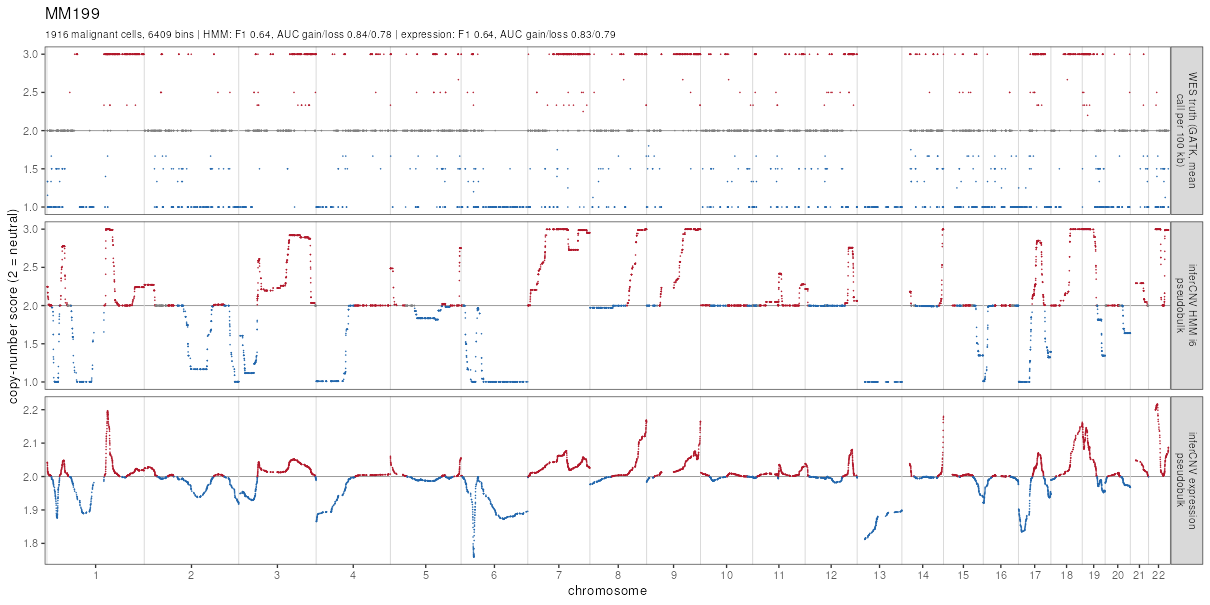
\includegraphics[width=\textwidth]{figures/fig4_MM199_genome.png}
\caption{\textbf{Comparison with DNA-based copy number in multiple myeloma MM199 (10x).} Top, whole-exome copy number segments (Schmid et al.~truth). Below, inferCNV pseudobulk scores over 1,916 malignant cells: HMM states after Bayesian filtering (CNV score) and final residual expression (expression score), in 100-kb bins along the genome. \todo{Panel with ROC curves and metric summary, if wanted; RESULT PENDING: BCH869 panel against WGS clone copy number.} Settings as in Methods.}
\label{fig:4}
\end{figure}

\begin{figure}[p]
\centering
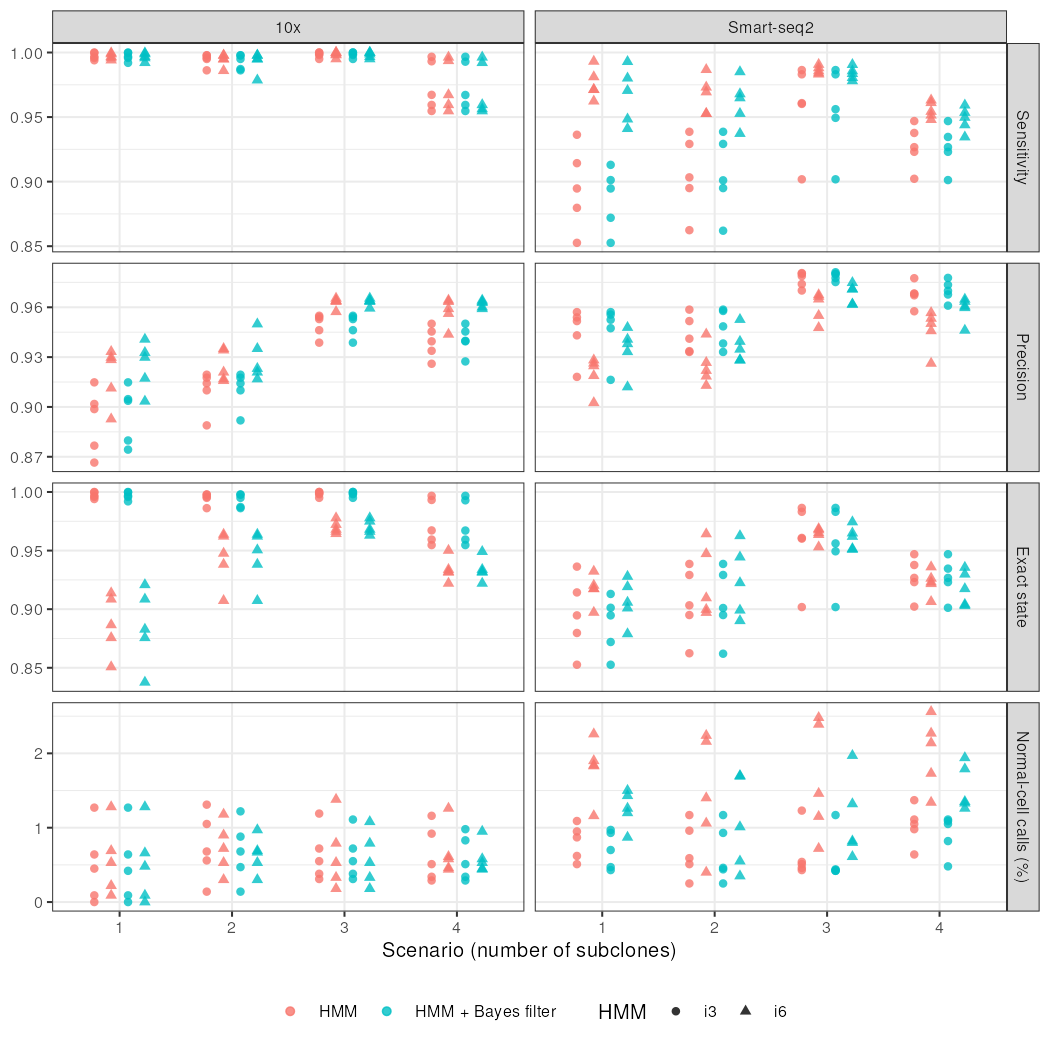
\includegraphics[width=\textwidth]{figures/fig5_simulation.png}
\caption{\textbf{Accuracy on simulated tumours.} Sensitivity, precision, exact-state accuracy, reference call rate and subcluster purity of the i6 HMM after Bayesian filtering for simulated 10x and Smart-seq2 data with one to four subclones (sim1--sim4), over five seeds (points) with means (bars); values in Table 1. \todo{Optional inset: i3 against i6.} \todo{Figure drawn from analyses/simulation/fig5\_simulation.png; check that it shows the master-build numbers of Table 1.}}
\label{fig:5}
\end{figure}

\begin{figure}[p]
\centering
\fbox{\parbox[c][4cm][c]{0.9\textwidth}{\centering Figure 6 pending}}
\caption{\textbf{Specificity and scale.} \todo{RESULT PENDING} (a) Non-neutral call rate in PBMC from healthy donors, by cell type, before and after Bayesian filtering. (b) Run time and peak memory against number of cells, with and without the Bayesian model and for i6 and i3.}
\label{fig:6}
\end{figure}

\begin{figure}[p]
\centering
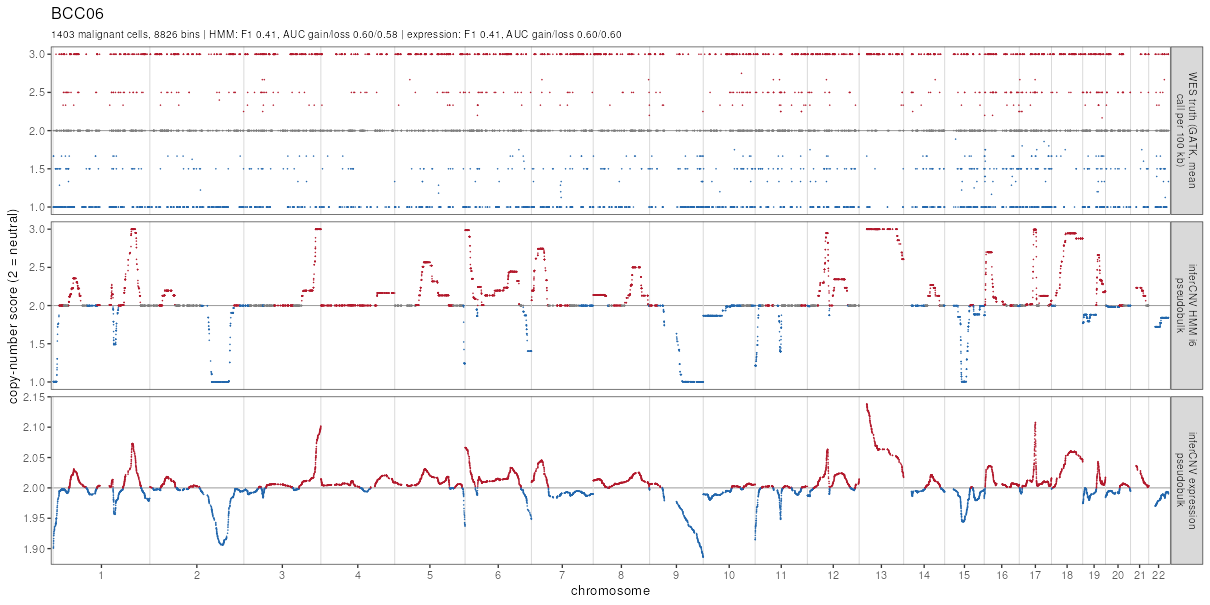
\includegraphics[width=\textwidth]{figures/figS1_BCC06_genome.png}
\caption{\textbf{Basal cell carcinoma BCC06 before and after treatment.} As Fig. 4, for BCC06 (1,403 malignant and 33 reference cells) and BCC06post (320 malignant and 280 reference cells). The exome segmentation of these samples is highly fragmented; see text.}
\label{fig:S1}
\end{figure}

% Supplementary Table S2: Metrics against DNA-based copy number.
% For each sample and score: number of malignant cells and bins, maximal F1, sensitivity and precision for gains and losses at the optimum, AUC and partial AUC for gains and losses, Pearson r; with the values reported by Schmid et al.~for inferCNV v1.10. (From analyses/fig4/metrics\_fig4.tsv and schmid2025\_reported\_infercnv\_v1.10.tsv.)
               -> figure
% The figure is emitted by the macro, not at \input time, so that it is numbered after the
% other supplementary figures.
%
% Everything below was derived from the release code (branch allele_integration):
% R/inferCNV_hidden_spike.R, R/inferCNV_meanVarSim.R, R/inferCNV_simple_sim.R (dropout fit),
% R/inferCNV_HMM.R, R/inferCNV_i3HMM.R, R/inferCNV_BayesNet.R, inst/BUGS_Mixture_Model{,_i3};
% allele-aware: R/inferCNV_allele.R, R/inferCNV_allele_HMM.R, R/inferCNV_allele_native.R,
% R/inferCNV_allele_BayesNet.R, R/inferCNV_combined_BayesNet.R. HoneyBADGER comparison: notes/honeybadger_lineage.md.

\subsection*{Generative models of the expression track: h-spike simulation, hidden Markov models and Bayesian mixture}
\label{sec:supp_models}

This section gives the models of steps 3, 19 and 20--21 in full (Supplementary Fig.~\ref{fig:Smodels}). Throughout, $x_{ij}$ is the residual expression of gene $i$ (in genomic order) in cell $j$ after step 16 (and step 18, if outlier pruning is on), on the fold-change scale with 1 as neutral; this is the matrix on which the HMM and the Bayesian model operate. A cell group $c$ (a subcluster by default, or an annotation group, or a single cell) has $n_c$ cells and mean residual $\bar x_{ic} = n_c^{-1}\sum_{j\in c} x_{ij}$. The i6 states $k=1,\dots,6$ correspond to the simulated levels $c_k\in\{0.01, 0.5, 1, 1.5, 2, 3\}$ (0 to $\geq$5 copies; $k=3$ neutral); the i3 states to loss, neutral and gain ($k=2$ neutral).

\paragraph{h-spike simulation (step 3, i6 only).}
Let $y_{ij}$ be the depth-normalised counts of step 3. For every annotation group $a$ (each observation group and each reference group) and gene $i$, the mean $m_{ia}$, variance $v_{ia}$ and zero fraction $p^0_{ia}$ over the group's cells are computed, and two smoothing splines (\texttt{smooth.spline}, smoothing parameter by generalised cross-validation) are fitted over all (gene, group) pairs: $f_v$ to $\log(v_{ia}+1)$ against $\log(m_{ia}+1)$, and $f_0$ to $p^0_{ia}$ against $\log m_{ia}$ (genes with $m_{ia}>0$). Both trends are thus estimated from all cells, observations included; only the gene means come from the reference cells. The synthetic genome has 11 chromosomes with copy factors $c_r = (1, 0.01, 1, 0.5, 1, 1.5, 1, 2, 1, 3, 1)$; the first ten have 400 genes each and the last $\max(G-4000, 400)$, where $G$ is the number of genes in the data, so that $G'=G$ genes whenever $G\geq 4400$. For each reference group $g$ (or the pooled references with \texttt{hspike\_aggregate\_normals}; all observations when there is no reference), each synthetic gene $i$ receives the mean of a data gene $\pi(i)$ drawn uniformly with replacement, $\tilde m_i = \max(m_{\pi(i) g}, 10^{-3})$, with the same $\pi$ for every group. Two sets of 100 cells are simulated, normal ($t=\mathrm{no}$) with $\mu^{(\mathrm{no})}_i=\tilde m_i$ and spiked ($t=\mathrm{sp}$) with $\mu^{(\mathrm{sp})}_i = c_{r(i)}\tilde m_i$. Counts are drawn independently for each gene and cell as a rounded, truncated normal with the variance predicted by the spline,
\begin{equation}
\tilde y_{ij} = \mathrm{round}\big(\max\{\,\mathcal N(\mu_i, s_i^2),\,0\}\big),\qquad
s_i^2 = \max\{\exp f_v(\log(\mu_i+1)) - 1,\ 0\},
\end{equation}
and dropout is then imposed per gene so that the zero fraction matches the trend: with $\pi_i = f_0(\log \bar{\tilde y}_{i\cdot})$ the predicted zero fraction at the simulated gene mean and $z_i$ the number of zeros already present among the $n=100$ cells, each nonzero $\tilde y_{ij}$ is set to zero independently with probability $\rho_i = \max\{(n\pi_i - z_i)/(n - z_i),\,0\}$. The resulting matrix $y^{\mathrm h}$ (200 cells per reference group) is depth-normalised to the median library size of the data and then carried through steps 6--16 in parallel with the data, with the simulated normal cells serving as the h-spike's own reference groups (it is not subclustered). The emission parameters of level $k$ are the mean and standard deviation of the pooled processed residuals $x^{\mathrm h}_{ij}$ of the spiked cells on the chromosomes with $c_r=c_k$ (the six neutral chromosomes are pooled for $k=3$):
\begin{equation}
\mu_k = \mathrm{mean}(P_k),\quad \sigma_k = \mathrm{sd}(P_k),\qquad P_k=\{x^{\mathrm h}_{ij}:\ c_{r(i)}=c_k,\ j\ \text{spiked}\}.
\end{equation}
To obtain the spread of a mean over $n$ cells, for $n=1,\dots,100$ the standard deviation $\hat\sigma_k(n)$ of the mean of $n$ values drawn with replacement from $P_k$ is estimated over 100 rounds (the $n=1$ point is undefined and dropped), and a line is fitted by least squares,
\begin{equation}
\log\hat\sigma_k(n) = a_k + b_k\log n,\qquad \sigma_k(n_c) = \exp(a_k + b_k\log n_c),
\end{equation}
with $b_k\approx-\tfrac12$ (Fig.~\ref{fig:2}f). The means $\mu_k$ are not scaled. In \texttt{analysis\_mode = "cells"} the single-cell $\sigma_k$ is used directly.

\paragraph{Hidden Markov model (step 19).}
For each chromosome with genes $i=1,\dots,L$ and each cell group $c$, the hidden states $s_i\in\{1,\dots,K\}$ ($K=6$ or 3) form a Markov chain with initial distribution $\delta$ and transition matrix $A$,
\begin{equation}
\Pr(s_1=k)=\delta_k,\qquad \Pr(s_{i+1}=l\mid s_i=k)=A_{kl},\qquad A_{kk}=1-(K-1)t,\quad A_{kl}=t\ (k\neq l),
\end{equation}
with $t=$ \texttt{HMM\_transition\_prob} $=10^{-6}$ and $\delta$ equal to $1-(K-1)t$ for the neutral state and $t$ otherwise. The emission model is Gaussian, $\bar x_{ic}\mid s_i=k \sim \mathcal N(\mu_k, \sigma_k(n_c)^2)$. For i6, $\mu_k$ and $\sigma_k(n_c)$ are the h-spike values above. For i3, with $R$ the set of residuals $x_{ij}$ of all reference cells (all cells when there is no reference), $\mu=\mathrm{mean}(R)$ and $\sigma=\mathrm{sd}(R)$ define the neutral state, the loss and gain means are $\mu\mp\Delta$ with
\begin{equation}
\Delta = \sigma\,\Phi^{-1}(1-p),\qquad p=\texttt{HMM\_i3\_pval}=0.05\ \ (\Delta = 1.645\,\sigma),
\end{equation}
and all three states share $\sigma$, which is not scaled with $n_c$. With \texttt{HMM\_i3\_use\_KS}, $\Delta$ is instead taken from a straight-line fit of the shift $d\in\{0,\sigma/10,\dots,\sigma\}$ on the mean two-sample Kolmogorov--Smirnov $p$-value (100 replicates) between $n_R$ draws from $\mathcal N(0,\sigma^2)$ and $n_R$ draws from $\mathcal N(d,\sigma^2)$, evaluated at $p$, where $n_R$ is the number of reference cells. The i3 model is the expression HMM of HoneyBADGER \citep{fan2018}, which has the same three states, the same transition probability and a common standard deviation; HoneyBADGER places the loss and gain means at a fixed $\mp m$ ($m=0.15$ by default) and takes the standard deviation from the group's mean profile, and the Kolmogorov--Smirnov calibration is its procedure (\texttt{setGexpDev}, with 101 draws per sample rather than $n_R$). HoneyBADGER runs the HMM on the groups obtained by cutting a hierarchical clustering of the cells at successive heights; inferCNV runs it on its subclusters.

The chain is decoded by the Viterbi algorithm. HoneyBADGER uses the standard algorithm of the HiddenMarkov package; the inferCNV implementation (\texttt{Viterbi.dthmm.adj}, adapted from the HiddenMarkov package \citep{hiddenmarkov}) departs from the textbook recursion in the emission term: the state standard deviations are replaced by their median, $\tilde\sigma_c = \mathrm{median}_k\,\sigma_k(n_c)$ (for i3, $\tilde\sigma_c=\sigma$), and the Gaussian density is replaced by a normalised score based on the one-sided tail probability of each state,
\begin{equation}
q_{ik} = 1-\Phi\!\left(\frac{|\bar x_{ic}-\mu_k|}{\tilde\sigma_c}\right),\qquad
b_{ik} = \frac{(-\log q_{ik})^{-1}}{\sum_{l=1}^{K}(-\log q_{il})^{-1}},
\label{eq:emission}
\end{equation}
so that $b_{ik}$ is the relative, not absolute, support for state $k$ at gene $i$ and decays more slowly with distance from $\mu_k$ than a Gaussian. The recursion is $\nu_{1k} = \log\delta_k + \log b_{1k}$, $\nu_{ik} = \max_l\{\nu_{i-1,l} + \log A_{lk}\} + \log b_{ik}$, with the usual back-trace $\hat s_L=\arg\max_k \nu_{Lk}$ and $\hat s_i = \arg\max_k\{\nu_{ik}+\log A_{k\hat s_{i+1}}\}$. A chromosome with a single gene is assigned the neutral state. All cells of the group receive the group's state sequence; a region is a maximal run of consecutive genes of a chromosome with the same state in a group, and the states are mapped to the representative values 0, 0.5, 1, 1.5, 2, 3 (i6) or 0.5, 1, 1.5 (i3) for output.

\paragraph{Bayesian latent mixture model (steps 20--21).}
Re-examining each HMM region with a Bayesian model of its cells is HoneyBADGER's approach \citep{fan2018}: there, each cell of a region is either unaltered or altered, with one direction of change per region and a change of fixed magnitude, and the model is fitted in JAGS. inferCNV generalises it to a mixture over all $K$ HMM states. Each HMM region $r$ with genes $G_r$, called in cell group $c$, is modelled with the cells $C_r$ of that group ($|C_r|=n_c$) as a finite mixture of the $K$ state distributions with known components (model files \texttt{inst/BUGS\_Mixture\_Model} for i6 and \texttt{inst/BUGS\_Mixture\_Model\_i3} for i3):
\begin{equation}
\theta \sim \mathrm{Dirichlet}(1,\dots,1),\qquad
\varepsilon_j \mid \theta \sim \mathrm{Categorical}(\theta),\qquad
x_{ij}\mid \varepsilon_j=k \sim \mathcal N(\mu_k, \tau_k^{-1}),\quad i\in G_r,\ j\in C_r,
\end{equation}
with the state means $\mu_k$ and precisions $\tau_k=\sigma_k^{-2}$ fixed: for i6 the single-cell h-spike values ($\sigma_k$, not $\sigma_k(n_c)$, because the model describes individual cells), and for i3 the means $\mu-\Delta,\mu,\mu+\Delta$ with common precision $\sigma^{-2}$, where $\Delta$ is always the $p$-value shift ($\texttt{HMM\_i3\_use\_KS}$ affects only the HMM). Genes within a cell are conditionally independent given the cell's state, and residuals are assumed independent across cells (Supplementary Fig.~\ref{fig:Smodels}d).

Both full conditionals have closed forms. Given the states, the mixing proportions are $\theta\mid\varepsilon \sim \mathrm{Dirichlet}(1+n_1,\dots,1+n_K)$ with $n_k=\#\{j:\varepsilon_j=k\}$; given $\theta$, each cell's state has $\Pr(\varepsilon_j=k\mid\theta,x)\propto\theta_k\prod_{i\in G_r}\mathcal N(x_{ij};\mu_k,\tau_k^{-1})$, which depends on the data only through $\sum_i x_{ij}$ and $\sum_i x_{ij}^2$. Gibbs sampling alternates the two. The released code did this in JAGS \citep{plummer2003jags} through rjags \citep{rjags}; inferCNV now draws the same two conditionals directly in R (option \texttt{infercnv.bayes\_sampler = "native"}, the default; \texttt{"jags"} restores JAGS, which is also used for a user-supplied model file). $K$ chains are run, chain $k$ initialised with every cell in state $k$; 700 iterations are discarded (JAGS: 500 adaptation and 200 burn-in iterations; adaptation has no effect on these exact updates) and 1,000 are retained from each chain, and the $K\times 1{,}000$ draws are pooled. The chains are drawn together as one vectorised computation from R's generator, so that a run with \texttt{seed} set is reproducible. On the TNBC1 data, the posterior probabilities of the neutral state from the R sampler and from JAGS agreed closely over the 1,913 regions (Pearson $r=0.99993$; largest difference 0.0096), 1,912 filtering decisions were identical (the remaining region had probabilities of 0.499 and 0.501), and on four threads the sampling took 3 instead of 49 minutes (8.8 instead of 55 minutes with the posterior summaries).

The region-level posterior probability of state $k$ is the posterior mean of the mixing proportion, $P_r(k)=\mathbb E[\theta_k\mid x]$, and the cell-level probability $P_{rj}(k)=\Pr(\varepsilon_j=k\mid x)$ is the fraction of draws in which cell $j$ is in state $k$. Because the components are fixed, $P_r(k)\approx(\bar n_k+1)/(n_c+K)$, where $\bar n_k$ is the posterior mean number of cells in state $k$: it is essentially the fraction of the group's cells whose residuals over $G_r$ are best explained by state $k$, shrunk towards $1/K$ by the prior. (One consequence is that with i6 a region in a group of four or fewer cells cannot reach $P_r(\text{neutral})>0.5$ even if every cell looks neutral.) The residuals are smoothed over about 100 genes, so neighbouring genes of a cell are strongly correlated, whereas the model multiplies their likelihoods as if they were independent. The per-cell posteriors are therefore over-confident, usually close to 0 or 1, and are better read as hard assignments than as calibrated probabilities; $P_r(k)$ is affected less, because it depends mainly on how many cells are assigned to each state. Filtering (step 21) resets a region to neutral when $P_r(\text{neutral})>$ \texttt{BayesMaxPNormal}; otherwise, with \texttt{reassignCNVs}, its state becomes $\arg\max_k P_r(k)$, which can itself be the neutral state. The cell-level probabilities are plotted and stored in the output object, but are not used for filtering.

\subsection*{Allele-aware models}
\label{sec:supp_allele}

When allele counts are supplied, inferCNV adds the allelic imbalance of heterozygous single-nucleotide polymorphisms (SNPs) to the expression signal (steps 2, 4--5 and 23--28; Supplementary Fig.~\ref{fig:Sallele}). Allelic imbalance shows events that expression cannot: copy-neutral loss of heterozygosity (LOH), and which kind of change underlies an expression shift. The extension, written by Yu Zhong, follows HoneyBADGER \citep{fan2018} closely. Its allele HMM is HoneyBADGER's, and the allele-only and combined Bayesian models of the release were ports of HoneyBADGER's allele model and joint expression--allele model, extended to the inferCNV states. For this paper we revised the two Bayesian models; they are described below, followed by the changes from the release. The data preparation, the allele HMM and the fusion of expression and allele segments are as released.

\paragraph{Allele data (steps 2, 4 and 5).}
\texttt{CreateInfercnvObject()} takes, besides the expression counts, two SNP $\times$ cell matrices: the alternative-allele read counts (\texttt{raw\_allele\_matrix}) and the total read counts (\texttt{raw\_coverage\_matrix}), with SNPs named by chromosome and position. In step 2, a SNP is kept as heterozygous if at least \texttt{min\_cells\_per\_snp} (default 3) reference cells have an alternative-allele fraction below 0.5 and at least as many have one above 0.5 (all cells are used when there is no reference). Entries with coverage below \texttt{snp\_min\_coverage} (default 0, i.e.\ off) are set to zero. For each SNP, the counts are then re-expressed as those of its \emph{lesser} allele, the allele that is in the minority in most of the observation cells that cover it; inferCNV thus needs no phasing. HoneyBADGER orients each SNP in the same way, from the allele fraction of a bulk or pooled ``in-silico bulk'' sample. Below, $r_{sj}$ is the lesser-allele count and $n_{sj}$ the total count of SNP $s$ in cell $j$. In step 4 each SNP is assigned to the nearest gene of the gene order file, including SNPs between genes. With \texttt{allele\_mode = "gene\_level"}, step 5 keeps, for each gene and cell, the SNP with the highest coverage (\texttt{collapse\_method = "highest"}), so that the models below run on one value per gene; the default, \texttt{"snp\_level"}, keeps all SNPs.

\paragraph{Allele HMM (step 23).}
For each subcluster $c$ with at least two cells and each chromosome, the allele HMM segments the SNPs, in genomic order, into allelically imbalanced and balanced stretches (Supplementary Fig.~\ref{fig:Sallele}a). The observation at SNP $s$ is the number of the subcluster's cells that show the lesser allele at all, $m_{sc}=\#\{j\in c: r_{sj}>0\}$, out of the number of cells that cover the SNP, $N_{sc}=\#\{j\in c: n_{sj}>0\}$. With one or two reads per cell, as is typical, a covered cell of a balanced region shows the lesser allele about half the time, whereas in a region that has lost one allele it shows it only through errors or contaminating cells. The two hidden states $z_s$ therefore have emissions
\begin{equation}
m_{sc}\mid z_s \sim \mathrm{Binomial}(N_{sc}, p_{z_s}),\qquad p_{\mathrm{imbalanced}} = 0.1,\quad p_{\mathrm{balanced}}=0.45,
\end{equation}
with transition probability $t=10^{-6}$ and initial probabilities $(\tfrac12,\tfrac12)$. The chain is decoded by the Viterbi algorithm, with the binomial probabilities floored at $t$ and normalised over the two states. Runs of at least five consecutive imbalanced SNPs are kept, and every SNP within the genomic span of a kept run is marked imbalanced for the cells of the subcluster. The model and all its constants are those of HoneyBADGER's \texttt{calcAlleleCnvBoundaries}. HoneyBADGER also trims 10\% of the SNPs from each run and runs the HMM on groups from successive cuts of a hierarchical clustering; inferCNV does not trim and uses its subclusters.

\paragraph{Allele-only Bayesian model (steps 24--25).}
As for expression, each allele-HMM region $r$, with SNPs $S_r$ and the cells $C_r$ of the subcluster in which it was called, is re-examined with a mixture model over its cells (Supplementary Fig.~\ref{fig:Sallele}b). Each cell is either allelically imbalanced or balanced, $\varepsilon_j\mid\theta\sim\mathrm{Categorical}(\theta)$ with $\theta\sim\mathrm{Dirichlet}(1,1)$. Each state is a set of genotypes with an expected lesser-allele fraction $f$. The imbalanced state covers the genotypes that lose one allele (one-copy loss or copy-neutral LOH; $f=\epsilon=0.01$, allowing for errors) and those that gain one (three copies, $f=\tfrac13$; four copies split 3:1, $f=\tfrac14$), each with equal prior weight; the balanced state has $f=\tfrac12$. Write $f_j$ for the fraction of the genotype of cell $j$. The lesser allele of step 2 is defined over all tumour cells and need not be the allele reduced in this subclone, so each SNP of the region has a latent orientation $a_s\sim\mathrm{Bernoulli}(\tfrac12)$, shared by all cells of the region:
\begin{equation}
p_{sj} = a_s f_j + (1-a_s)(1-f_j),\qquad
r_{sj}\mid n_{sj} \sim \mathrm{BetaBinomial}\big(n_{sj},\ \kappa p_{sj},\ \kappa(1-p_{sj})\big),
\end{equation}
over the SNP--cell pairs with coverage. Because the orientation is shared, imbalance must favour the same allele of each SNP in every cell of the state, which separates a genomic loss from random monoallelic expression of individual cells. The beta-binomial allows the reads of a cell at a SNP to be more variable than independent draws, as transcriptional bursting and other sources of allelic overdispersion make them; it has mean $p_{sj}$ and concentration $\kappa$. $\kappa$ is fitted once per run by maximum likelihood over all covered SNP--cell pairs of the reference cells with $p=\tfrac12$, where heterozygous SNPs are balanced (on the TNBC1 data, $\kappa=21.7$ from 302 reference cells). When the reference cells have fewer than 50 covered pairs, for example when they come from another sample without allele data, $\kappa$ is fitted on all cells with each SNP's mean set to its pooled lesser-allele fraction (clipped to $[0.01, 0.99]$), so that imbalance from CNAs is not mistaken for overdispersion; with fewer than 50 pairs in all, $\kappa=10$. In step 25, a region is reset to balanced when $P_r(\text{balanced})>$ \texttt{BayesMaxPNormal}, and kept as imbalanced otherwise. With \texttt{allele\_mode = "gene\_level"}, $s$ runs over the region's genes, each with the counts of its chosen SNP.

\paragraph{Fusion of expression and allele segments (step 26).}
For each subcluster, the regions remaining after the expression filter (step 21) and the allele filter (step 25) are cut into disjoint segments. Each segment takes the expression state of the region that covers it (neutral if none) and the allele state (balanced if none). The segment's combined state is the expression state, except that allelic imbalance with neutral expression becomes copy-neutral LOH (state 7 with i6, 4 with i3), and allelic imbalance with a 0-copy expression state, which is contradictory because no allele is expressed, is flagged as state 8 (i6). Each gene takes the state of the first segment it overlaps. With \texttt{combined\_method = "common"} instead of the default \texttt{"union"}, only genes with SNPs are kept. In the release, the fusion read the unfiltered HMM reports of steps 19 and 23, so the two filters had no effect on the combined result.

\paragraph{Combined expression and allele model (steps 27--28).}
Each fused region $r$, with genes $G_r$, the SNPs $S_r$ assigned to those genes and the cells $C_r$ of its subcluster, is fitted with a mixture over copy-number states in which each cell's state must explain both its expression and its alleles (Supplementary Fig.~\ref{fig:Sallele}c). HoneyBADGER's joint model has the same structure, with one cell-level indicator of an altered state; here the states are those of the HMM plus copy-neutral LOH: for i6, 0, 1, 2, 3, 4 and $\geq$5 copies and copy-neutral LOH; for i3, loss, neutral, gain and copy-neutral LOH. Each state has genotypes with lesser-allele fractions $f$:
\begin{center}
\small
\begin{tabular}{lll}
\hline
i6 state & genotypes & $f$\\
\hline
0 copies & -- & $\tfrac12$ (no allelic information; reads are ambient or from other cells)\\
1 copy & (1,0) & $\epsilon$\\
2 copies & (1,1) & $\tfrac12$\\
3 copies & (2,1) & $\tfrac13$\\
4 copies & (2,2), (3,1) & $\tfrac12$, $\tfrac14$\\
$\geq$5 copies & e.g.\ (3,3), (4,2), (5,1) & $\tfrac12$, $\tfrac13$, $\tfrac16$\\
copy-neutral LOH & (2,0) & $\epsilon$\\
\hline
\end{tabular}
\end{center}
For i3, loss has $f=\epsilon$, neutral $f=\tfrac12$, gain $f\in\{\tfrac12,\tfrac13,\tfrac14\}$ and copy-neutral LOH $f=\epsilon$. The genotypes of a state have equal prior weight. The allele likelihood, the orientations $a_s$ and $\kappa$ are as in the allele-only model. For expression, the model uses each cell's mean residual over the region, $\bar x_j = |G_r|^{-1}\sum_{i\in G_r}x_{ij}$:
\begin{equation}
\bar x_j\mid \varepsilon_j=k \sim \mathcal N\!\left(\mu_k,\ \big(s_r\,\sigma_k/\sigma_{\mathrm{neutral}}\big)^2\right),
\end{equation}
where $\mu_k$ and $\sigma_k$ are the single-cell state means and standard deviations of the expression model (h-spike for i6, reference residuals for i3), copy-neutral LOH takes the neutral values, and $s_r$ is the standard deviation of the same region mean across the reference cells (the single-cell $\sigma_{\mathrm{neutral}}$ when there are fewer than five). Smoothing makes neighbouring genes nearly identical, so the per-gene likelihood of the expression-only model would count the expression evidence of a large region many times over and swamp the alleles; the region mean, with its spread measured on reference cells, gives expression the weight it actually has. A region without SNPs is fitted with the expression term alone and without the copy-neutral LOH state. In step 28 a region is reset to neutral when $P_r(\text{neutral})>$ \texttt{BayesMaxPNormal}; otherwise it takes its most probable state, which may be copy-neutral LOH.

\paragraph{Sampling.}
Both allele-aware models are fitted by Gibbs sampling in R. Each sweep draws, for every cell, its state and genotype jointly from their categorical full conditional given $\theta$ and the orientations; then $\theta$ from its Dirichlet full conditional; then each orientation $a_s$ from its Bernoulli full conditional, whose log-odds are the summed differences, over the cells of a non-balanced genotype, between the beta-binomial log-likelihoods of $r_{sj}$ at $f_j$ and at $1-f_j$. One chain is run per state, initialised with all cells in that state and all $a_s=1$, with 700 iterations discarded and 1,000 retained. The per-SNP likelihood terms are computed once per region, so a sweep costs time proportional to the number of covered SNP--cell pairs. On simulated regions with 10x-like and Smart-seq2-like coverage, the combined model assigned neutral, one-copy loss, three-copy gain and copy-neutral LOH regions to the correct state.

\paragraph{Changes from the release.}
The release fitted ports of HoneyBADGER's BUGS models in JAGS. In the allele-only model, a balanced cell had, for every gene, either a SNP-specific allele probability with a nearly flat prior (truncated $\mathcal N(0.5, \text{precision } 0.1)$ on $[0.1, 0.9]$) or, with prior probability 0.7, monoallelic expression in a random direction; an imbalanced cell had a lesser-allele probability of 0.1. A ``bulk'' binomial term determined the orientation of each SNP. In HoneyBADGER the bulk counts come from a separate bulk sample or from all cells; in the release they were recomputed from the cells being modelled, so that the same reads entered twice. The combined model extended this to the i6 or i3 states with an added copy-neutral LOH state. Only the 1-copy and copy-neutral LOH states were imbalanced, so an imbalanced gain (for example 2:1) could be explained by the alleles only as LOH. Each gene's expression residual entered as an independent observation. The revised models replace the per-gene allele model with the beta-binomial, fitted on reference cells, and the bulk term with the shared orientations $a_s$, which play the same part. They give the gain states their imbalanced genotypes, and use the region mean for expression. The release versions remain available with \texttt{options(infercnv.bayes\_sampler = "jags")}.

% ------------------------------------------------------------------
% The figure. Emitted where \SuppModelsFigure is called (after sections/figures.tex).
% TikZ bodies of the model diagrams (Supplementary Fig. \ref{fig:Smodels}).
% Shared by sections/supp_models.tex (via \SuppModelsFigure) and figures/plates_standalone.tex.
% Requires: \usepackage{tikz} \usetikzlibrary{bayesnet,positioning,fit,arrows,calc}
%
% Node conventions (tikz-bayesnet): latent = white circle (random), obs = grey circle
% (observed / given data), det = diamond (deterministic function of its parents),
% const = plain text (fixed quantity). Plates = replication.

\tikzset{
  mnode/.style={font=\footnotesize},
  plate caption/.append style={font=\scriptsize},
  note/.style={font=\scriptsize, text=black!70, align=left, inner sep=1pt},
  >=stealth,
}

% ------------------------------------------------------------------
% (a) h-spike simulator (one reference group g)
% ------------------------------------------------------------------
\newcommand{\PlateHspike}{%
\begin{tikzpicture}[node distance=0.5cm and 0.7cm, mnode]
  % given data and the quantities derived from it
  \node[obs]                                  (Y)  {$y$};
  \node[note, above=0.05cm of Y, align=center] {depth-normalised counts,\\all annotation groups};
  \node[det, below=0.5cm of Y] (m)  {$m_g$};
  \node[note, right=0.05cm of m] {gene means,\\ref.\ group $g$};
  \edge{Y}{m};
  % genes plate
  \node[det, below=0.7cm of m]          (mt)  {$\tilde m_i$};
  \node[const, right=0.7cm of mt]       (c)   {$c_{r(i)}$};
  \node[det, below=of mt]               (mu)  {$\mu^{(t)}_i$};
  \node[latent, below=0.6cm of mu]      (yt)  {$\tilde y_{ij}$};
  \node[latent, below=0.6cm of yt]      (yd)  {$y^{\mathrm h}_{ij}$};
  \edge{m}{mt}; \edge{mt}{mu}; \edge{c}{mu}; \edge{mu}{yt}; \edge{yt}{yd};
  \plate[inner sep=0.16cm]{cells}{(yt)(yd)}{$j=1,\dots,100$}
  \plate[inner sep=0.22cm]{type}{(cells)}{$t\in\{\mathrm{no},\mathrm{sp}\}$}
  \plate[inner sep=0.26cm]{genes}{(mt)(c)(mu)(type)}{$i=1,\dots,G'$}
  % splines, outside the plates, feeding the simulated counts
  \node[det, left=1.6cm of yt] (fv) {$f_v$};
  \node[det, left=1.6cm of yd] (f0) {$f_0$};
  \node[note, left=0.05cm of fv, align=right] {mean--variance\\spline};
  \node[note, left=0.05cm of f0, align=right] {mean--dropout\\spline};
  % edges from the data run left at the height of y, then down (right of the spline nodes)
  \draw[->] (Y.west) -| (fv.north);
  \draw[->] (Y.west) -| ($(f0.north east)+(0.25,0.35)$) -- (f0.north east);
  \edge{fv}{yt}; \edge{f0}{yd};
  % downstream
  \node[det, below=0.8cm of genes] (x) {$x^{\mathrm h}_{ij}$};
  \node[note, right=0.1cm of x] {residuals after steps 6--16,\\mirrored on the h-spike};
  \draw[->] (genes.south) -- (x);
  \node[const, below=0.45cm of x] (par) {$\mu_k,\ \sigma_k,\ \sigma_k(n)$};
  \node[note, right=0.1cm of par] {per level $k$, from the spiked cells\\of the chromosomes with $c_r=c_k$};
  \edge{x}{par};
\end{tikzpicture}}

% ------------------------------------------------------------------
% HMM chain on one chromosome of one cell group c (shared by the i6 and i3 diagrams)
% ------------------------------------------------------------------
\newcommand{\HMMchain}{%
  \node[const]                          (delta) {$\delta$};
  \node[latent, below=0.5cm of delta]   (s1) {$s_1$};
  \node[latent, below=of s1]            (s2) {$s_2$};
  \node[latent, below=of s2]            (s3) {$s_3$};
  \node[below=0.2cm of s3]              (dots) {$\vdots$};
  \node[latent, below=0.2cm of dots]    (sL) {$s_L$};
  \node[obs, right=of s1] (x1) {$\bar x_{1c}$};
  \node[obs, right=of s2] (x2) {$\bar x_{2c}$};
  \node[obs, right=of s3] (x3) {$\bar x_{3c}$};
  \node[obs, right=of sL] (xL) {$\bar x_{Lc}$};
  \edge{delta}{s1}; \edge{s3}{dots}; \edge{dots}{sL};
  \draw[->] (s1) -- node[left, font=\scriptsize] {$A$} (s2);
  \draw[->] (s2) -- node[left, font=\scriptsize] {$A$} (s3);
  \edge{s1}{x1}; \edge{s2}{x2}; \edge{s3}{x3}; \edge{sL}{xL};
  \plate[inner sep=0.2cm]{chr}{(s1)(sL)(x1)(xL)}{$i=1,\dots,L$}}

% ------------------------------------------------------------------
% (b) six-state HMM (i6): emission parameters from the h-spike
% ------------------------------------------------------------------
\newcommand{\PlateHMMsix}{%
\begin{tikzpicture}[node distance=0.45cm and 0.6cm, mnode]
  \HMMchain
  \node[const, right=0.5cm of chr.east, align=center] (par) {$\mu_k$\\$\sigma_k(n_c)$};
  \edge{par}{x1}; \edge{par}{x2}; \edge{par}{x3}; \edge{par}{xL};
  \plate[inner sep=0.26cm]{grp}{(chr)(delta)(par)}{group $c$; chromosomes}
  \node[note, below=0.1cm of grp, text width=4.4cm] {$K=6$ states, $k=3$ neutral; $\mu_k$, $\sigma_k(n_c)$ from the h-spike (a); $\bar x_{ic}$: mean residual of the $n_c$ cells of group $c$ at gene $i$; $A_{kk}=1-5t$, $A_{kl}=t$.};
\end{tikzpicture}}

% ------------------------------------------------------------------
% (c) three-state HMM (i3): emission parameters from the reference residuals
% ------------------------------------------------------------------
\newcommand{\PlateHMMthree}{%
\begin{tikzpicture}[node distance=0.45cm and 0.6cm, mnode]
  \HMMchain
  \node[det, right=0.5cm of chr.east] (par) {$\mu_k,\sigma$};
  \node[det, right=0.5cm of par, yshift=0.9cm]  (mus) {$\mu,\sigma$};
  \node[det, right=0.5cm of par, yshift=-0.9cm] (Del) {$\Delta$};
  \node[obs, above=0.5cm of mus]                (R)   {$R$};
  \node[note, above=0.02cm of R, align=center] {reference\\residuals};
  \node[const, below=0.45cm of Del]             (pv)  {$p$};
  \edge{R}{mus}; \edge{mus}{Del}; \edge{pv}{Del}; \edge{mus}{par}; \edge{Del}{par};
  \edge{par}{x1}; \edge{par}{x2}; \edge{par}{x3}; \edge{par}{xL};
  \plate[inner sep=0.26cm]{grp}{(chr)(delta)}{group $c$; chromosomes}
  \node[note, below=0.1cm of grp, text width=4.6cm] {$K=3$ states (loss, neutral, gain) with means $\mu-\Delta,\ \mu,\ \mu+\Delta$ and common $\sigma$, not scaled with $n_c$; $\Delta=\sigma\Phi^{-1}(1-p)$ or the KS shift; $A_{kk}=1-2t$.};
\end{tikzpicture}}

% ------------------------------------------------------------------
% (d) Bayesian latent mixture model for one HMM region r (i6 and i3)
% ------------------------------------------------------------------
\newcommand{\PlateBayes}{%
\begin{tikzpicture}[node distance=0.5cm and 0.8cm, mnode]
  \node[const]                        (alpha) {$\alpha=(1,\dots,1)$};
  \node[latent, below=0.45cm of alpha] (theta) {$\theta$};
  \node[latent, below=of theta]       (eps)   {$\varepsilon_j$};
  \node[obs, below=of eps]            (x)     {$x_{ij}$};
  \edge{alpha}{theta}; \edge{theta}{eps}; \edge{eps}{x};
  \plate[inner sep=0.16cm]{genes}{(x)}{$i\in G_r$}
  \plate[inner sep=0.24cm]{cells}{(eps)(genes)}{$j\in C_r$}
  \plate[inner sep=0.3cm]{region}{(theta)(cells)}{region $r$}
  % fixed state parameters, shared by all regions
  \node[const, right=1.8cm of x, yshift=0.3cm]  (mu)  {$\mu_k$};
  \node[const, below=0.2cm of mu]               (tau) {$\tau_k$};
  \edge{mu}{x}; \edge{tau}{x};
  \plate[inner sep=0.14cm]{K}{(mu)(tau)}{$K$ states}
  \node[note, below=0.1cm of region, text width=4.4cm] {$\mu_k$, $\tau_k=\sigma_k^{-2}$ fixed (i6: single-cell h-spike values; i3: $\mu\mp\Delta$, $\mu$, $\sigma$). $P_r(k)=\mathbb E[\theta_k\mid x]$, $P_{rj}(k)=\Pr(\varepsilon_j=k\mid x)$.};
\end{tikzpicture}}

% ==================================================================
% Allele-aware models (Supplementary Fig. \ref{fig:Sallele})
% ==================================================================

% ------------------------------------------------------------------
% (a) allele HMM on one chromosome of one subcluster c (step 23)
% ------------------------------------------------------------------
\newcommand{\PlateAlleleHMM}{%
\begin{tikzpicture}[node distance=0.45cm and 0.55cm, mnode]
  \node[const]                          (delta) {$\delta$};
  \node[latent, below=0.5cm of delta]   (z1) {$z_1$};
  \node[latent, below=of z1]            (z2) {$z_2$};
  \node[below=0.2cm of z2]              (dots) {$\vdots$};
  \node[latent, below=0.2cm of dots]    (zL) {$z_L$};
  \node[obs, right=of z1] (m1) {$m_{1c}$};
  \node[obs, right=of z2] (m2) {$m_{2c}$};
  \node[obs, right=of zL] (mL) {$m_{Lc}$};
  \edge{delta}{z1}; \edge{z2}{dots}; \edge{dots}{zL};
  \draw[->] (z1) -- node[left, font=\scriptsize] {$A$} (z2);
  \edge{z1}{m1}; \edge{z2}{m2}; \edge{zL}{mL};
  \node[obs, right=0.45cm of m1] (N1) {$N_{1c}$};
  \node[obs, right=0.45cm of m2] (N2) {$N_{2c}$};
  \node[obs, right=0.45cm of mL] (NL) {$N_{Lc}$};
  \edge{N1}{m1}; \edge{N2}{m2}; \edge{NL}{mL};
  \node[below=0.35cm of mL, inner sep=0pt, minimum size=0pt] (padL) {};
  \plate[inner sep=0.2cm]{chr}{(z1)(zL)(m1)(mL)(N1)(NL)(padL)}{SNPs $s=1,\dots,L$}
  \node[const, right=0.5cm of chr.east] (pp) {$p_{\mathrm{d}},p_{\mathrm{n}}$};
  \coordinate (bus) at ($(chr.east)+(0.2,0)$);
  \draw (pp.west) -- (bus);
  \draw[->] (bus) |- ($(m1.north)+(0,0.3)$) -- (m1.north);
  \draw[->] (bus) |- ($(mL.south)+(0,-0.25)$) -- (mL.south);
  \plate[inner sep=0.26cm]{grp}{(chr)(delta)(pp)}{subcluster $c$; chromosomes}
  \node[note, below=0.1cm of grp, text width=5.0cm] {$z_s\in\{$imbalanced, balanced$\}$; of the $N_{sc}$ cells of $c$ covering SNP $s$, $m_{sc}$ show the lesser allele: $m_{sc}\sim\mathrm{Bin}(N_{sc}, p_{z_s})$, $p_{\mathrm d}=0.1$, $p_{\mathrm n}=0.45$; $A_{kk}=1-t$; $\delta=(\tfrac12,\tfrac12)$.};
\end{tikzpicture}}

% ------------------------------------------------------------------
% (b) allele-only Bayesian mixture for one allele-HMM region r (step 24)
% ------------------------------------------------------------------
\newcommand{\PlateAlleleMix}{%
\begin{tikzpicture}[node distance=0.5cm and 0.6cm, mnode]
  \node[const]                          (alpha) {$\alpha=(1,1)$};
  \node[latent, below=0.4cm of alpha]   (theta) {$\theta$};
  \node[latent, below=of theta]         (eps)   {$\varepsilon_j$};
  \node[latent, below=of eps]           (f)     {$f_j$};
  \node[det, below=0.6cm of f]          (p)     {$p_{sj}$};
  \node[obs, below=0.5cm of p]          (r)     {$r_{sj}$};
  \node[obs, left=0.5cm of r]           (n)     {$n_{sj}$};
  \edge{alpha}{theta}; \edge{theta}{eps}; \edge{eps}{f}; \edge{f}{p}; \edge{p}{r}; \edge{n}{r};
  \plate[inner sep=0.14cm]{snpsin}{(p)(r)(n)}{$s\in S_r$}
  \plate[inner sep=0.22cm]{cells}{(eps)(f)(snpsin)}{$j\in C_r$}
  \node[latent, right=1.3cm of p]       (a)     {$a_s$};
  \plate[inner sep=0.14cm]{snpsout}{(a)}{$s\in S_r$}
  \edge{a}{p};
  \node[const, right=1.3cm of r]        (kap)   {$\kappa$};
  \node[note, below=0.05cm of kap, align=center] {fitted on\\reference cells};
  \edge{kap}{r};
  \plate[inner sep=0.3cm]{region}{(theta)(cells)(snpsout)}{region $r$}
  \node[note, below=0.1cm of region, text width=5.2cm] {$\varepsilon_j\in\{$imbalanced, balanced$\}$; $f_j$: expected lesser-allele fraction of the cell's genotype (imbalanced: $\epsilon$, $\tfrac13$ or $\tfrac14$; balanced: $\tfrac12$); $a_s$: which allele of SNP $s$ is in the minority, shared by all cells; $p_{sj}=f_j$ if $a_s=1$, else $1-f_j$; $r_{sj}\sim\mathrm{BetaBin}(n_{sj},\kappa p_{sj},\kappa(1-p_{sj}))$.};
\end{tikzpicture}}

% ------------------------------------------------------------------
% (c) combined expression + allele Bayesian mixture for one fused region r (step 27)
% ------------------------------------------------------------------
\newcommand{\PlateCombined}{%
\begin{tikzpicture}[node distance=0.5cm and 0.6cm, mnode]
  \node[const]                          (alpha) {$\alpha=(1,\dots,1)$};
  \node[latent, below=0.4cm of alpha]   (theta) {$\theta$};
  \node[latent, below=of theta]         (eps)   {$\varepsilon_j$};
  \node[latent, below=of eps]           (f)     {$f_j$};
  \node[det, below=0.6cm of f]          (p)     {$p_{sj}$};
  \node[obs, below=0.5cm of p]          (r)     {$r_{sj}$};
  \node[obs, left=0.5cm of r]           (n)     {$n_{sj}$};
  \node[obs, left=1.1cm of f]           (x)     {$\bar x_j$};
  \edge{alpha}{theta}; \edge{theta}{eps}; \edge{eps}{f}; \edge{f}{p}; \edge{p}{r}; \edge{n}{r};
  \edge{eps}{x};
  \plate[inner sep=0.14cm]{snpsin}{(p)(r)(n)}{$s\in S_r$}
  \plate[inner sep=0.22cm]{cells}{(eps)(f)(snpsin)(x)}{$j\in C_r$}
  \node[latent, right=1.3cm of p]       (a)     {$a_s$};
  \plate[inner sep=0.14cm]{snpsout}{(a)}{$s\in S_r$}
  \edge{a}{p};
  \node[const, right=1.3cm of r]        (kap)   {$\kappa$};
  \edge{kap}{r};
  \plate[inner sep=0.3cm]{region}{(theta)(cells)(snpsout)}{region $r$}
  % expression parameters
  \node[const, left=1.6cm of x, yshift=0.7cm, align=center] (mu) {$\mu_k,\sigma_k$};
  \node[note, left=0.05cm of mu, align=right] {h-spike (i6) or\\reference (i3)};
  \node[obs, left=1.6cm of x, yshift=-0.9cm] (sref) {$s_r$};
  \node[note, left=0.05cm of sref, align=right] {spread of the\\region mean in\\reference cells};
  \edge{mu}{x}; \edge{sref}{x};
  \node[note, below=0.1cm of region, text width=6.6cm] {$\varepsilon_j$: copy-number state (i6: 0, 1, 2, 3, 4, $\geq$5 copies and copy-neutral LOH; i3: loss, neutral, gain, copy-neutral LOH); $f_j$: lesser-allele fraction of one of the state's genotypes (e.g.\ 3 copies: $\tfrac13$; LOH and 1 copy: $\epsilon$); $\bar x_j$: the cell's mean residual over the region's genes, $\bar x_j\sim\mathcal N\big(\mu_{\varepsilon_j},\,(s_r\sigma_{\varepsilon_j}/\sigma_{\mathrm{neutral}})^2\big)$; allele terms as in b.};
\end{tikzpicture}}

\providecommand{\PlateScale}{0.68}
\newcommand{\SuppModelsFigure}{%
\begin{figure}[p]
\centering
\begin{minipage}[t]{0.49\textwidth}
  \textbf{a}\quad h-spike simulator (i6)\\[2pt]
  \scalebox{\PlateScale}{\PlateHspike}
\end{minipage}\hfill
\begin{minipage}[t]{0.49\textwidth}
  \textbf{b}\quad six-state HMM (i6)\\[2pt]
  \scalebox{\PlateScale}{\PlateHMMsix}
\end{minipage}\\[4pt]
\begin{minipage}[t]{0.49\textwidth}
  \textbf{c}\quad three-state HMM (i3)\\[2pt]
  \scalebox{\PlateScale}{\PlateHMMthree}
\end{minipage}\hfill
\begin{minipage}[t]{0.49\textwidth}
  \textbf{d}\quad Bayesian latent mixture (i6 and i3)\\[2pt]
  \scalebox{\PlateScale}{\PlateBayes}
\end{minipage}
\captionsetup{font={footnotesize,stretch=1}}
\caption{\textbf{Graphical models of the expression track: the i6 calibration, the two HMMs and the Bayesian filter.} Circles are random variables (grey: given data), diamonds deterministic quantities, plain symbols fixed parameters, and boxes replication (plates). \textbf{a}, h-spike simulator (step 3; one reference group $g$): mean--variance and mean--dropout splines ($f_v$, $f_0$) are fitted to the depth-normalised counts $y$, and the reference gene means $m_g$ are sampled to give $\tilde m_i$ on a synthetic genome with copy factors $c_r$; counts of 100 normal and 100 spiked cells are simulated, processed exactly as the data, and their residuals $x^{\mathrm h}_{ij}$ give each level's emission mean $\mu_k$, single-cell standard deviation $\sigma_k$ and group-size scaling $\sigma_k(n)$. \textbf{b}, Six-state HMM for one chromosome of one cell group $c$ (step 19): hidden states $s_i$ with initial distribution $\delta$ and transition matrix $A$ (off-diagonal $t=10^{-6}$), emitting the group's mean residual $\bar x_{ic}$ from $\mathcal N(\mu_k,\sigma_k(n_c)^2)$ with the h-spike parameters of panel a; decoded by Viterbi with the emission score of Eq.~\ref{eq:emission}. \textbf{c}, Three-state HMM, HoneyBADGER's design \citep{fan2018}: the same chain, with the neutral mean $\mu$ and standard deviation $\sigma$ of the reference residuals $R$, loss and gain means $\mu\mp\Delta$ with $\Delta$ set by the tail probability $p$ (or the Kolmogorov--Smirnov criterion), and a standard deviation not scaled with group size. \textbf{d}, Bayesian latent mixture model for one HMM region $r$ (steps 20--21), for either HMM: the cells $C_r$ of the group have states $\varepsilon_j$ drawn from mixing proportions $\theta$ with a flat Dirichlet prior, and the residuals $x_{ij}$ of the region's genes $G_r$ are normal with the fixed mean and precision of the cell's state (i6: single-cell h-spike values; i3: those of panel c). The posterior mean of $\theta$ gives the region's state probabilities, and the posterior of $\varepsilon_j$ the cell-level probabilities.}
\label{fig:Smodels}
\end{figure}}

\newcommand{\SuppAlleleFigure}{%
\begin{figure}[p]
\centering
\begin{minipage}[t]{0.44\textwidth}
  \textbf{a}\quad allele HMM\\[2pt]
  \scalebox{\PlateScale}{\PlateAlleleHMM}
\end{minipage}\hfill
\begin{minipage}[t]{0.53\textwidth}
  \textbf{b}\quad allele-only mixture\\[2pt]
  \scalebox{\PlateScale}{\PlateAlleleMix}
\end{minipage}\\[8pt]
\begin{minipage}[t]{0.8\textwidth}
  \textbf{c}\quad combined expression and allele mixture\\[2pt]
  \scalebox{\PlateScale}{\PlateCombined}
\end{minipage}
\captionsetup{font={footnotesize,stretch=1}}
\caption{\textbf{Graphical models of the allele-aware track.} Conventions as in Supplementary Fig.~\ref{fig:Smodels}. \textbf{a}, Allele HMM for one chromosome of one subcluster $c$ (step 23), HoneyBADGER's model \citep{fan2018}: hidden states $z_s$ (imbalanced or balanced) along the heterozygous SNPs, emitting the number $m_{sc}$ of covering cells that show the lesser allele, out of the $N_{sc}$ cells that cover SNP $s$. \textbf{b}, Allele-only Bayesian mixture for one allele-HMM region $r$ (steps 24--25): each cell $j$ of the subcluster is imbalanced or balanced ($\varepsilon_j$), with a genotype of expected lesser-allele fraction $f_j$; the lesser-allele count $r_{sj}$ of the $n_{sj}$ reads is beta-binomial with mean $p_{sj}$, which is $f_j$ or $1-f_j$ according to the SNP's orientation $a_s$, shared by all cells (a separate plate over the same SNPs), and concentration $\kappa$ fitted on the reference cells. \textbf{c}, Combined model for one fused region (steps 27--28): the cell's copy-number state $\varepsilon_j$ (including copy-neutral LOH) determines both the distribution of its mean residual over the region, $\bar x_j$, with the state's mean and the region's reference spread $s_r$, and its genotype and allele counts, as in b. b and c are the models revised for this paper; the release used ports of HoneyBADGER's allele and joint models (Supplementary Methods).}
\label{fig:Sallele}
\end{figure}}
      after \section{Supplementary Methods}\label{sec:supplementary_methods}

A step-by-step description of \texttt{run()}, with all defaults, branch conditions, checkpoint file names and resume behaviour, and with references to the source code, is given in Supplementary Methods (manuscript/supplementary\_algorithm.md). Its step numbers follow the expression-only pipeline of 22 steps. In the release, which also contains the allele model, two allele steps are inserted after depth normalisation, so steps 4--20 of the expression pipeline become steps 6--22, the allele and combined-model steps are 23--28, and the masking of non-differentially expressed genes and denoising become steps 29 and 30. \todo{Supplement to be renumbered or given a mapping table before posting.}
  -> text
%   \SuppModelsFigure                 after \begin{figure}[p]
\centering
\fbox{\parbox[c][4cm][c]{0.9\textwidth}{\centering Figure 1 pending}}
\caption{\textbf{The inferCNV workflow.} \todo{RESULT PENDING} Schematic of the expression model with heatmap snapshots from the 183-cell oligodendroglioma example data set (observations above, reference cells below; columns are genes ordered by genomic position). (a) Log-transformed counts after gene filtering and depth normalisation. (b) Residual expression after subtraction of the reference and smoothing along each chromosome. (c) After per-cell centering. (d) After the second reference subtraction, shown on the fold-change scale. (e) After denoising (\texttt{denoise\ =\ TRUE}). (f) i6 HMM state predictions per subcluster after Bayesian filtering, computed from the fold-change-scale residuals in (d) after subclustering. Panels (e) and (f) are alternative outputs derived from (d).}
\label{fig:1}
\end{figure}

\begin{figure}[p]
\centering
\fbox{\parbox[c][4cm][c]{0.9\textwidth}{\centering Figure 2 pending}}
\caption{\textbf{In-silico spike-in (h-spike) calibration of the HMM.} \todo{RESULT PENDING} (a) Mean--variance and (b) mean--dropout relationships of the reference cells with spline fits used to simulate counts. (c) Residual expression of the simulated h-spike chromosomes after the same processing as the real data, at relative copy number levels 0.01, 0.5, 1, 1.5, 2 and 3; the per-level distributions define the i6 emission parameters. (d) Comparison of i6 and i3 state calls on the same tumour.}
\label{fig:2}
\end{figure}

\begin{figure}[p]
\centering
\fbox{\parbox[c][4cm][c]{0.9\textwidth}{\centering Figure 3 pending}}
\caption{\textbf{inferCNV applied to tumours profiled with Smart-seq2.} \todo{RESULT PENDING} Residual expression heatmaps (top) and i6 HMM predictions with subclusters (bottom) for (a) oligodendroglioma, (b) glioblastoma, (c) melanoma and (d) H3K27M glioma. (e) \todo{or Supplementary Fig. S2} Synovial sarcoma: SS18--SSX fusion detection in cells classified as malignant or non-malignant by inferCNV.}
\label{fig:3}
\end{figure}

\begin{figure}[p]
\centering
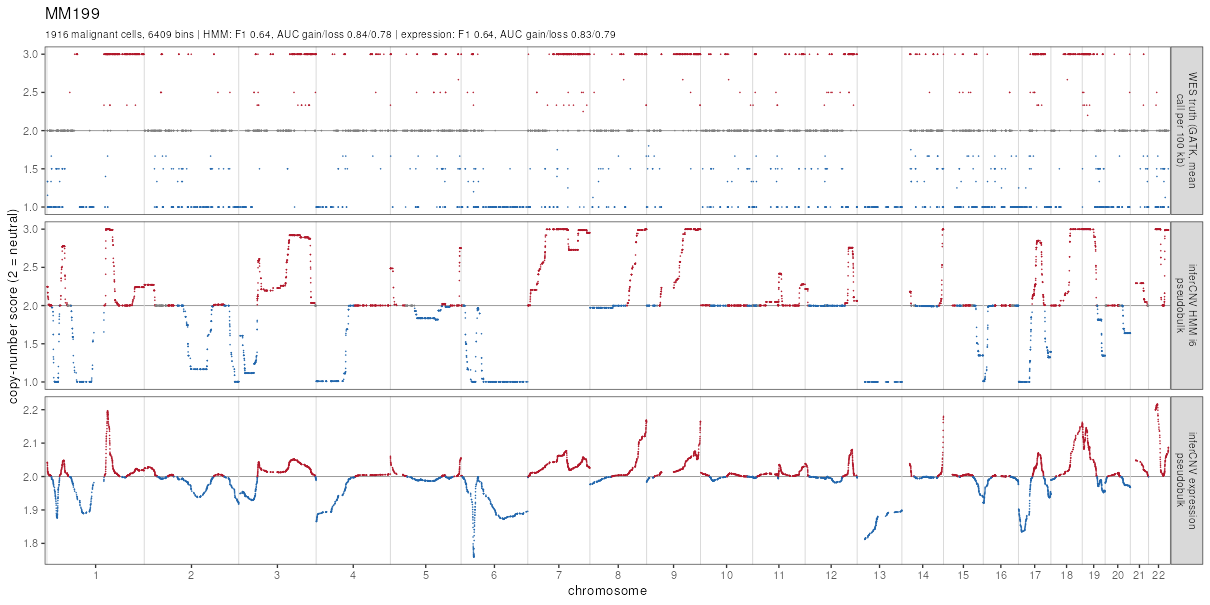
\includegraphics[width=\textwidth]{figures/fig4_MM199_genome.png}
\caption{\textbf{Comparison with DNA-based copy number in multiple myeloma MM199 (10x).} Top, whole-exome copy number segments (Schmid et al.~truth). Below, inferCNV pseudobulk scores over 1,916 malignant cells: HMM states after Bayesian filtering (CNV score) and final residual expression (expression score), in 100-kb bins along the genome. \todo{Panel with ROC curves and metric summary, if wanted; RESULT PENDING: BCH869 panel against WGS clone copy number.} Settings as in Methods.}
\label{fig:4}
\end{figure}

\begin{figure}[p]
\centering
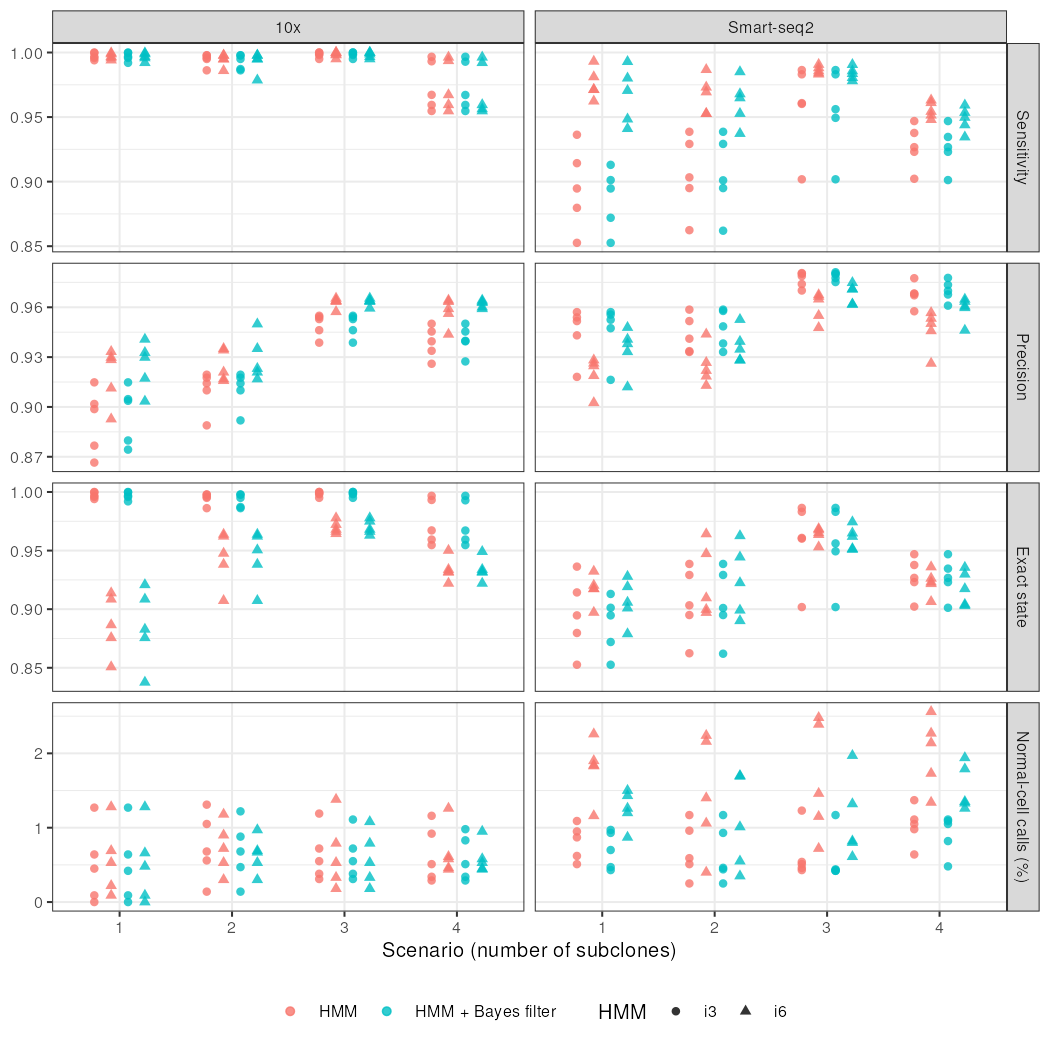
\includegraphics[width=\textwidth]{figures/fig5_simulation.png}
\caption{\textbf{Accuracy on simulated tumours.} Sensitivity, precision, exact-state accuracy, reference call rate and subcluster purity of the i6 HMM after Bayesian filtering for simulated 10x and Smart-seq2 data with one to four subclones (sim1--sim4), over five seeds (points) with means (bars); values in Table 1. \todo{Optional inset: i3 against i6.} \todo{Figure drawn from analyses/simulation/fig5\_simulation.png; check that it shows the master-build numbers of Table 1.}}
\label{fig:5}
\end{figure}

\begin{figure}[p]
\centering
\fbox{\parbox[c][4cm][c]{0.9\textwidth}{\centering Figure 6 pending}}
\caption{\textbf{Specificity and scale.} \todo{RESULT PENDING} (a) Non-neutral call rate in PBMC from healthy donors, by cell type, before and after Bayesian filtering. (b) Run time and peak memory against number of cells, with and without the Bayesian model and for i6 and i3.}
\label{fig:6}
\end{figure}

\begin{figure}[p]
\centering
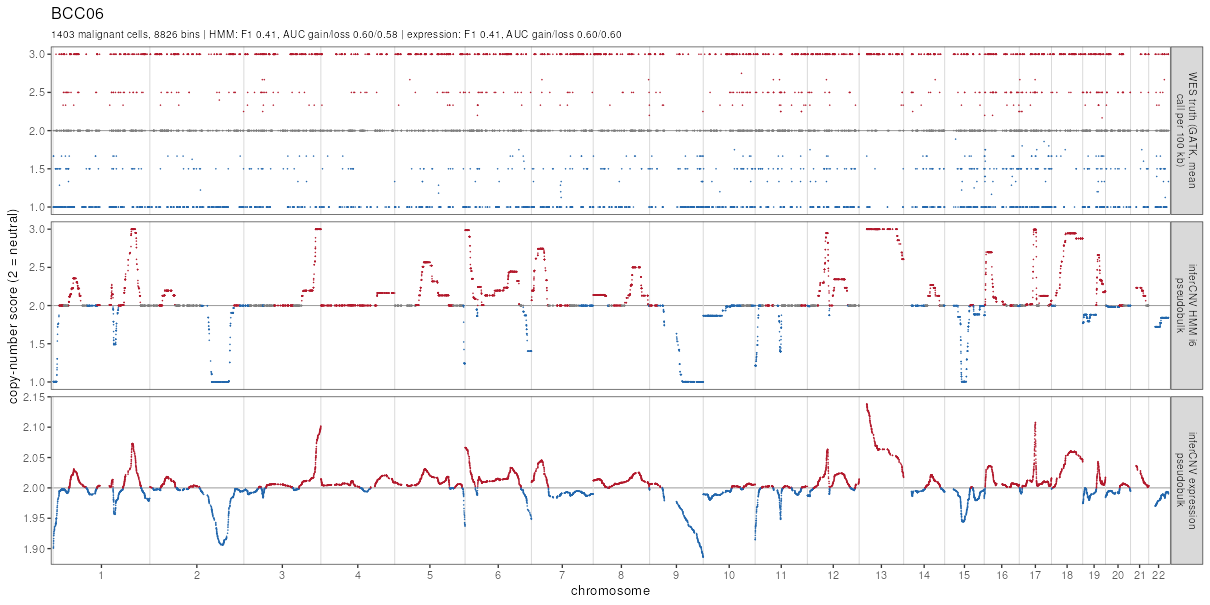
\includegraphics[width=\textwidth]{figures/figS1_BCC06_genome.png}
\caption{\textbf{Basal cell carcinoma BCC06 before and after treatment.} As Fig. 4, for BCC06 (1,403 malignant and 33 reference cells) and BCC06post (320 malignant and 280 reference cells). The exome segmentation of these samples is highly fragmented; see text.}
\label{fig:S1}
\end{figure}

% Supplementary Table S2: Metrics against DNA-based copy number.
% For each sample and score: number of malignant cells and bins, maximal F1, sensitivity and precision for gains and losses at the optimum, AUC and partial AUC for gains and losses, Pearson r; with the values reported by Schmid et al.~for inferCNV v1.10. (From analyses/fig4/metrics\_fig4.tsv and schmid2025\_reported\_infercnv\_v1.10.tsv.)
               -> figure
% The figure is emitted by the macro, not at \input time, so that it is numbered after the
% other supplementary figures.
%
% Everything below was derived from the release code (branch allele_integration):
% R/inferCNV_hidden_spike.R, R/inferCNV_meanVarSim.R, R/inferCNV_simple_sim.R (dropout fit),
% R/inferCNV_HMM.R, R/inferCNV_i3HMM.R, R/inferCNV_BayesNet.R, inst/BUGS_Mixture_Model{,_i3};
% allele-aware: R/inferCNV_allele.R, R/inferCNV_allele_HMM.R, R/inferCNV_allele_native.R,
% R/inferCNV_allele_BayesNet.R, R/inferCNV_combined_BayesNet.R. HoneyBADGER comparison: notes/honeybadger_lineage.md.

\subsection*{Generative models of the expression track: h-spike simulation, hidden Markov models and Bayesian mixture}
\label{sec:supp_models}

This section gives the models of steps 3, 19 and 20--21 in full (Supplementary Fig.~\ref{fig:Smodels}). Throughout, $x_{ij}$ is the residual expression of gene $i$ (in genomic order) in cell $j$ after step 16 (and step 18, if outlier pruning is on), on the fold-change scale with 1 as neutral; this is the matrix on which the HMM and the Bayesian model operate. A cell group $c$ (a subcluster by default, or an annotation group, or a single cell) has $n_c$ cells and mean residual $\bar x_{ic} = n_c^{-1}\sum_{j\in c} x_{ij}$. The i6 states $k=1,\dots,6$ correspond to the simulated levels $c_k\in\{0.01, 0.5, 1, 1.5, 2, 3\}$ (0 to $\geq$5 copies; $k=3$ neutral); the i3 states to loss, neutral and gain ($k=2$ neutral).

\paragraph{h-spike simulation (step 3, i6 only).}
Let $y_{ij}$ be the depth-normalised counts of step 3. For every annotation group $a$ (each observation group and each reference group) and gene $i$, the mean $m_{ia}$, variance $v_{ia}$ and zero fraction $p^0_{ia}$ over the group's cells are computed, and two smoothing splines (\texttt{smooth.spline}, smoothing parameter by generalised cross-validation) are fitted over all (gene, group) pairs: $f_v$ to $\log(v_{ia}+1)$ against $\log(m_{ia}+1)$, and $f_0$ to $p^0_{ia}$ against $\log m_{ia}$ (genes with $m_{ia}>0$). Both trends are thus estimated from all cells, observations included; only the gene means come from the reference cells. The synthetic genome has 11 chromosomes with copy factors $c_r = (1, 0.01, 1, 0.5, 1, 1.5, 1, 2, 1, 3, 1)$; the first ten have 400 genes each and the last $\max(G-4000, 400)$, where $G$ is the number of genes in the data, so that $G'=G$ genes whenever $G\geq 4400$. For each reference group $g$ (or the pooled references with \texttt{hspike\_aggregate\_normals}; all observations when there is no reference), each synthetic gene $i$ receives the mean of a data gene $\pi(i)$ drawn uniformly with replacement, $\tilde m_i = \max(m_{\pi(i) g}, 10^{-3})$, with the same $\pi$ for every group. Two sets of 100 cells are simulated, normal ($t=\mathrm{no}$) with $\mu^{(\mathrm{no})}_i=\tilde m_i$ and spiked ($t=\mathrm{sp}$) with $\mu^{(\mathrm{sp})}_i = c_{r(i)}\tilde m_i$. Counts are drawn independently for each gene and cell as a rounded, truncated normal with the variance predicted by the spline,
\begin{equation}
\tilde y_{ij} = \mathrm{round}\big(\max\{\,\mathcal N(\mu_i, s_i^2),\,0\}\big),\qquad
s_i^2 = \max\{\exp f_v(\log(\mu_i+1)) - 1,\ 0\},
\end{equation}
and dropout is then imposed per gene so that the zero fraction matches the trend: with $\pi_i = f_0(\log \bar{\tilde y}_{i\cdot})$ the predicted zero fraction at the simulated gene mean and $z_i$ the number of zeros already present among the $n=100$ cells, each nonzero $\tilde y_{ij}$ is set to zero independently with probability $\rho_i = \max\{(n\pi_i - z_i)/(n - z_i),\,0\}$. The resulting matrix $y^{\mathrm h}$ (200 cells per reference group) is depth-normalised to the median library size of the data and then carried through steps 6--16 in parallel with the data, with the simulated normal cells serving as the h-spike's own reference groups (it is not subclustered). The emission parameters of level $k$ are the mean and standard deviation of the pooled processed residuals $x^{\mathrm h}_{ij}$ of the spiked cells on the chromosomes with $c_r=c_k$ (the six neutral chromosomes are pooled for $k=3$):
\begin{equation}
\mu_k = \mathrm{mean}(P_k),\quad \sigma_k = \mathrm{sd}(P_k),\qquad P_k=\{x^{\mathrm h}_{ij}:\ c_{r(i)}=c_k,\ j\ \text{spiked}\}.
\end{equation}
To obtain the spread of a mean over $n$ cells, for $n=1,\dots,100$ the standard deviation $\hat\sigma_k(n)$ of the mean of $n$ values drawn with replacement from $P_k$ is estimated over 100 rounds (the $n=1$ point is undefined and dropped), and a line is fitted by least squares,
\begin{equation}
\log\hat\sigma_k(n) = a_k + b_k\log n,\qquad \sigma_k(n_c) = \exp(a_k + b_k\log n_c),
\end{equation}
with $b_k\approx-\tfrac12$ (Fig.~\ref{fig:2}f). The means $\mu_k$ are not scaled. In \texttt{analysis\_mode = "cells"} the single-cell $\sigma_k$ is used directly.

\paragraph{Hidden Markov model (step 19).}
For each chromosome with genes $i=1,\dots,L$ and each cell group $c$, the hidden states $s_i\in\{1,\dots,K\}$ ($K=6$ or 3) form a Markov chain with initial distribution $\delta$ and transition matrix $A$,
\begin{equation}
\Pr(s_1=k)=\delta_k,\qquad \Pr(s_{i+1}=l\mid s_i=k)=A_{kl},\qquad A_{kk}=1-(K-1)t,\quad A_{kl}=t\ (k\neq l),
\end{equation}
with $t=$ \texttt{HMM\_transition\_prob} $=10^{-6}$ and $\delta$ equal to $1-(K-1)t$ for the neutral state and $t$ otherwise. The emission model is Gaussian, $\bar x_{ic}\mid s_i=k \sim \mathcal N(\mu_k, \sigma_k(n_c)^2)$. For i6, $\mu_k$ and $\sigma_k(n_c)$ are the h-spike values above. For i3, with $R$ the set of residuals $x_{ij}$ of all reference cells (all cells when there is no reference), $\mu=\mathrm{mean}(R)$ and $\sigma=\mathrm{sd}(R)$ define the neutral state, the loss and gain means are $\mu\mp\Delta$ with
\begin{equation}
\Delta = \sigma\,\Phi^{-1}(1-p),\qquad p=\texttt{HMM\_i3\_pval}=0.05\ \ (\Delta = 1.645\,\sigma),
\end{equation}
and all three states share $\sigma$, which is not scaled with $n_c$. With \texttt{HMM\_i3\_use\_KS}, $\Delta$ is instead taken from a straight-line fit of the shift $d\in\{0,\sigma/10,\dots,\sigma\}$ on the mean two-sample Kolmogorov--Smirnov $p$-value (100 replicates) between $n_R$ draws from $\mathcal N(0,\sigma^2)$ and $n_R$ draws from $\mathcal N(d,\sigma^2)$, evaluated at $p$, where $n_R$ is the number of reference cells. The i3 model is the expression HMM of HoneyBADGER \citep{fan2018}, which has the same three states, the same transition probability and a common standard deviation; HoneyBADGER places the loss and gain means at a fixed $\mp m$ ($m=0.15$ by default) and takes the standard deviation from the group's mean profile, and the Kolmogorov--Smirnov calibration is its procedure (\texttt{setGexpDev}, with 101 draws per sample rather than $n_R$). HoneyBADGER runs the HMM on the groups obtained by cutting a hierarchical clustering of the cells at successive heights; inferCNV runs it on its subclusters.

The chain is decoded by the Viterbi algorithm. HoneyBADGER uses the standard algorithm of the HiddenMarkov package; the inferCNV implementation (\texttt{Viterbi.dthmm.adj}, adapted from the HiddenMarkov package \citep{hiddenmarkov}) departs from the textbook recursion in the emission term: the state standard deviations are replaced by their median, $\tilde\sigma_c = \mathrm{median}_k\,\sigma_k(n_c)$ (for i3, $\tilde\sigma_c=\sigma$), and the Gaussian density is replaced by a normalised score based on the one-sided tail probability of each state,
\begin{equation}
q_{ik} = 1-\Phi\!\left(\frac{|\bar x_{ic}-\mu_k|}{\tilde\sigma_c}\right),\qquad
b_{ik} = \frac{(-\log q_{ik})^{-1}}{\sum_{l=1}^{K}(-\log q_{il})^{-1}},
\label{eq:emission}
\end{equation}
so that $b_{ik}$ is the relative, not absolute, support for state $k$ at gene $i$ and decays more slowly with distance from $\mu_k$ than a Gaussian. The recursion is $\nu_{1k} = \log\delta_k + \log b_{1k}$, $\nu_{ik} = \max_l\{\nu_{i-1,l} + \log A_{lk}\} + \log b_{ik}$, with the usual back-trace $\hat s_L=\arg\max_k \nu_{Lk}$ and $\hat s_i = \arg\max_k\{\nu_{ik}+\log A_{k\hat s_{i+1}}\}$. A chromosome with a single gene is assigned the neutral state. All cells of the group receive the group's state sequence; a region is a maximal run of consecutive genes of a chromosome with the same state in a group, and the states are mapped to the representative values 0, 0.5, 1, 1.5, 2, 3 (i6) or 0.5, 1, 1.5 (i3) for output.

\paragraph{Bayesian latent mixture model (steps 20--21).}
Re-examining each HMM region with a Bayesian model of its cells is HoneyBADGER's approach \citep{fan2018}: there, each cell of a region is either unaltered or altered, with one direction of change per region and a change of fixed magnitude, and the model is fitted in JAGS. inferCNV generalises it to a mixture over all $K$ HMM states. Each HMM region $r$ with genes $G_r$, called in cell group $c$, is modelled with the cells $C_r$ of that group ($|C_r|=n_c$) as a finite mixture of the $K$ state distributions with known components (model files \texttt{inst/BUGS\_Mixture\_Model} for i6 and \texttt{inst/BUGS\_Mixture\_Model\_i3} for i3):
\begin{equation}
\theta \sim \mathrm{Dirichlet}(1,\dots,1),\qquad
\varepsilon_j \mid \theta \sim \mathrm{Categorical}(\theta),\qquad
x_{ij}\mid \varepsilon_j=k \sim \mathcal N(\mu_k, \tau_k^{-1}),\quad i\in G_r,\ j\in C_r,
\end{equation}
with the state means $\mu_k$ and precisions $\tau_k=\sigma_k^{-2}$ fixed: for i6 the single-cell h-spike values ($\sigma_k$, not $\sigma_k(n_c)$, because the model describes individual cells), and for i3 the means $\mu-\Delta,\mu,\mu+\Delta$ with common precision $\sigma^{-2}$, where $\Delta$ is always the $p$-value shift ($\texttt{HMM\_i3\_use\_KS}$ affects only the HMM). Genes within a cell are conditionally independent given the cell's state, and residuals are assumed independent across cells (Supplementary Fig.~\ref{fig:Smodels}d).

Both full conditionals have closed forms. Given the states, the mixing proportions are $\theta\mid\varepsilon \sim \mathrm{Dirichlet}(1+n_1,\dots,1+n_K)$ with $n_k=\#\{j:\varepsilon_j=k\}$; given $\theta$, each cell's state has $\Pr(\varepsilon_j=k\mid\theta,x)\propto\theta_k\prod_{i\in G_r}\mathcal N(x_{ij};\mu_k,\tau_k^{-1})$, which depends on the data only through $\sum_i x_{ij}$ and $\sum_i x_{ij}^2$. Gibbs sampling alternates the two. The released code did this in JAGS \citep{plummer2003jags} through rjags \citep{rjags}; inferCNV now draws the same two conditionals directly in R (option \texttt{infercnv.bayes\_sampler = "native"}, the default; \texttt{"jags"} restores JAGS, which is also used for a user-supplied model file). $K$ chains are run, chain $k$ initialised with every cell in state $k$; 700 iterations are discarded (JAGS: 500 adaptation and 200 burn-in iterations; adaptation has no effect on these exact updates) and 1,000 are retained from each chain, and the $K\times 1{,}000$ draws are pooled. The chains are drawn together as one vectorised computation from R's generator, so that a run with \texttt{seed} set is reproducible. On the TNBC1 data, the posterior probabilities of the neutral state from the R sampler and from JAGS agreed closely over the 1,913 regions (Pearson $r=0.99993$; largest difference 0.0096), 1,912 filtering decisions were identical (the remaining region had probabilities of 0.499 and 0.501), and on four threads the sampling took 3 instead of 49 minutes (8.8 instead of 55 minutes with the posterior summaries).

The region-level posterior probability of state $k$ is the posterior mean of the mixing proportion, $P_r(k)=\mathbb E[\theta_k\mid x]$, and the cell-level probability $P_{rj}(k)=\Pr(\varepsilon_j=k\mid x)$ is the fraction of draws in which cell $j$ is in state $k$. Because the components are fixed, $P_r(k)\approx(\bar n_k+1)/(n_c+K)$, where $\bar n_k$ is the posterior mean number of cells in state $k$: it is essentially the fraction of the group's cells whose residuals over $G_r$ are best explained by state $k$, shrunk towards $1/K$ by the prior. (One consequence is that with i6 a region in a group of four or fewer cells cannot reach $P_r(\text{neutral})>0.5$ even if every cell looks neutral.) The residuals are smoothed over about 100 genes, so neighbouring genes of a cell are strongly correlated, whereas the model multiplies their likelihoods as if they were independent. The per-cell posteriors are therefore over-confident, usually close to 0 or 1, and are better read as hard assignments than as calibrated probabilities; $P_r(k)$ is affected less, because it depends mainly on how many cells are assigned to each state. Filtering (step 21) resets a region to neutral when $P_r(\text{neutral})>$ \texttt{BayesMaxPNormal}; otherwise, with \texttt{reassignCNVs}, its state becomes $\arg\max_k P_r(k)$, which can itself be the neutral state. The cell-level probabilities are plotted and stored in the output object, but are not used for filtering.

\subsection*{Allele-aware models}
\label{sec:supp_allele}

When allele counts are supplied, inferCNV adds the allelic imbalance of heterozygous single-nucleotide polymorphisms (SNPs) to the expression signal (steps 2, 4--5 and 23--28; Supplementary Fig.~\ref{fig:Sallele}). Allelic imbalance shows events that expression cannot: copy-neutral loss of heterozygosity (LOH), and which kind of change underlies an expression shift. The extension, written by Yu Zhong, follows HoneyBADGER \citep{fan2018} closely. Its allele HMM is HoneyBADGER's, and the allele-only and combined Bayesian models of the release were ports of HoneyBADGER's allele model and joint expression--allele model, extended to the inferCNV states. For this paper we revised the two Bayesian models; they are described below, followed by the changes from the release. The data preparation, the allele HMM and the fusion of expression and allele segments are as released.

\paragraph{Allele data (steps 2, 4 and 5).}
\texttt{CreateInfercnvObject()} takes, besides the expression counts, two SNP $\times$ cell matrices: the alternative-allele read counts (\texttt{raw\_allele\_matrix}) and the total read counts (\texttt{raw\_coverage\_matrix}), with SNPs named by chromosome and position. In step 2, a SNP is kept as heterozygous if at least \texttt{min\_cells\_per\_snp} (default 3) reference cells have an alternative-allele fraction below 0.5 and at least as many have one above 0.5 (all cells are used when there is no reference). Entries with coverage below \texttt{snp\_min\_coverage} (default 0, i.e.\ off) are set to zero. For each SNP, the counts are then re-expressed as those of its \emph{lesser} allele, the allele that is in the minority in most of the observation cells that cover it; inferCNV thus needs no phasing. HoneyBADGER orients each SNP in the same way, from the allele fraction of a bulk or pooled ``in-silico bulk'' sample. Below, $r_{sj}$ is the lesser-allele count and $n_{sj}$ the total count of SNP $s$ in cell $j$. In step 4 each SNP is assigned to the nearest gene of the gene order file, including SNPs between genes. With \texttt{allele\_mode = "gene\_level"}, step 5 keeps, for each gene and cell, the SNP with the highest coverage (\texttt{collapse\_method = "highest"}), so that the models below run on one value per gene; the default, \texttt{"snp\_level"}, keeps all SNPs.

\paragraph{Allele HMM (step 23).}
For each subcluster $c$ with at least two cells and each chromosome, the allele HMM segments the SNPs, in genomic order, into allelically imbalanced and balanced stretches (Supplementary Fig.~\ref{fig:Sallele}a). The observation at SNP $s$ is the number of the subcluster's cells that show the lesser allele at all, $m_{sc}=\#\{j\in c: r_{sj}>0\}$, out of the number of cells that cover the SNP, $N_{sc}=\#\{j\in c: n_{sj}>0\}$. With one or two reads per cell, as is typical, a covered cell of a balanced region shows the lesser allele about half the time, whereas in a region that has lost one allele it shows it only through errors or contaminating cells. The two hidden states $z_s$ therefore have emissions
\begin{equation}
m_{sc}\mid z_s \sim \mathrm{Binomial}(N_{sc}, p_{z_s}),\qquad p_{\mathrm{imbalanced}} = 0.1,\quad p_{\mathrm{balanced}}=0.45,
\end{equation}
with transition probability $t=10^{-6}$ and initial probabilities $(\tfrac12,\tfrac12)$. The chain is decoded by the Viterbi algorithm, with the binomial probabilities floored at $t$ and normalised over the two states. Runs of at least five consecutive imbalanced SNPs are kept, and every SNP within the genomic span of a kept run is marked imbalanced for the cells of the subcluster. The model and all its constants are those of HoneyBADGER's \texttt{calcAlleleCnvBoundaries}. HoneyBADGER also trims 10\% of the SNPs from each run and runs the HMM on groups from successive cuts of a hierarchical clustering; inferCNV does not trim and uses its subclusters.

\paragraph{Allele-only Bayesian model (steps 24--25).}
As for expression, each allele-HMM region $r$, with SNPs $S_r$ and the cells $C_r$ of the subcluster in which it was called, is re-examined with a mixture model over its cells (Supplementary Fig.~\ref{fig:Sallele}b). Each cell is either allelically imbalanced or balanced, $\varepsilon_j\mid\theta\sim\mathrm{Categorical}(\theta)$ with $\theta\sim\mathrm{Dirichlet}(1,1)$. Each state is a set of genotypes with an expected lesser-allele fraction $f$. The imbalanced state covers the genotypes that lose one allele (one-copy loss or copy-neutral LOH; $f=\epsilon=0.01$, allowing for errors) and those that gain one (three copies, $f=\tfrac13$; four copies split 3:1, $f=\tfrac14$), each with equal prior weight; the balanced state has $f=\tfrac12$. Write $f_j$ for the fraction of the genotype of cell $j$. The lesser allele of step 2 is defined over all tumour cells and need not be the allele reduced in this subclone, so each SNP of the region has a latent orientation $a_s\sim\mathrm{Bernoulli}(\tfrac12)$, shared by all cells of the region:
\begin{equation}
p_{sj} = a_s f_j + (1-a_s)(1-f_j),\qquad
r_{sj}\mid n_{sj} \sim \mathrm{BetaBinomial}\big(n_{sj},\ \kappa p_{sj},\ \kappa(1-p_{sj})\big),
\end{equation}
over the SNP--cell pairs with coverage. Because the orientation is shared, imbalance must favour the same allele of each SNP in every cell of the state, which separates a genomic loss from random monoallelic expression of individual cells. The beta-binomial allows the reads of a cell at a SNP to be more variable than independent draws, as transcriptional bursting and other sources of allelic overdispersion make them; it has mean $p_{sj}$ and concentration $\kappa$. $\kappa$ is fitted once per run by maximum likelihood over all covered SNP--cell pairs of the reference cells with $p=\tfrac12$, where heterozygous SNPs are balanced (on the TNBC1 data, $\kappa=21.7$ from 302 reference cells). When the reference cells have fewer than 50 covered pairs, for example when they come from another sample without allele data, $\kappa$ is fitted on all cells with each SNP's mean set to its pooled lesser-allele fraction (clipped to $[0.01, 0.99]$), so that imbalance from CNAs is not mistaken for overdispersion; with fewer than 50 pairs in all, $\kappa=10$. In step 25, a region is reset to balanced when $P_r(\text{balanced})>$ \texttt{BayesMaxPNormal}, and kept as imbalanced otherwise. With \texttt{allele\_mode = "gene\_level"}, $s$ runs over the region's genes, each with the counts of its chosen SNP.

\paragraph{Fusion of expression and allele segments (step 26).}
For each subcluster, the regions remaining after the expression filter (step 21) and the allele filter (step 25) are cut into disjoint segments. Each segment takes the expression state of the region that covers it (neutral if none) and the allele state (balanced if none). The segment's combined state is the expression state, except that allelic imbalance with neutral expression becomes copy-neutral LOH (state 7 with i6, 4 with i3), and allelic imbalance with a 0-copy expression state, which is contradictory because no allele is expressed, is flagged as state 8 (i6). Each gene takes the state of the first segment it overlaps. With \texttt{combined\_method = "common"} instead of the default \texttt{"union"}, only genes with SNPs are kept. In the release, the fusion read the unfiltered HMM reports of steps 19 and 23, so the two filters had no effect on the combined result.

\paragraph{Combined expression and allele model (steps 27--28).}
Each fused region $r$, with genes $G_r$, the SNPs $S_r$ assigned to those genes and the cells $C_r$ of its subcluster, is fitted with a mixture over copy-number states in which each cell's state must explain both its expression and its alleles (Supplementary Fig.~\ref{fig:Sallele}c). HoneyBADGER's joint model has the same structure, with one cell-level indicator of an altered state; here the states are those of the HMM plus copy-neutral LOH: for i6, 0, 1, 2, 3, 4 and $\geq$5 copies and copy-neutral LOH; for i3, loss, neutral, gain and copy-neutral LOH. Each state has genotypes with lesser-allele fractions $f$:
\begin{center}
\small
\begin{tabular}{lll}
\hline
i6 state & genotypes & $f$\\
\hline
0 copies & -- & $\tfrac12$ (no allelic information; reads are ambient or from other cells)\\
1 copy & (1,0) & $\epsilon$\\
2 copies & (1,1) & $\tfrac12$\\
3 copies & (2,1) & $\tfrac13$\\
4 copies & (2,2), (3,1) & $\tfrac12$, $\tfrac14$\\
$\geq$5 copies & e.g.\ (3,3), (4,2), (5,1) & $\tfrac12$, $\tfrac13$, $\tfrac16$\\
copy-neutral LOH & (2,0) & $\epsilon$\\
\hline
\end{tabular}
\end{center}
For i3, loss has $f=\epsilon$, neutral $f=\tfrac12$, gain $f\in\{\tfrac12,\tfrac13,\tfrac14\}$ and copy-neutral LOH $f=\epsilon$. The genotypes of a state have equal prior weight. The allele likelihood, the orientations $a_s$ and $\kappa$ are as in the allele-only model. For expression, the model uses each cell's mean residual over the region, $\bar x_j = |G_r|^{-1}\sum_{i\in G_r}x_{ij}$:
\begin{equation}
\bar x_j\mid \varepsilon_j=k \sim \mathcal N\!\left(\mu_k,\ \big(s_r\,\sigma_k/\sigma_{\mathrm{neutral}}\big)^2\right),
\end{equation}
where $\mu_k$ and $\sigma_k$ are the single-cell state means and standard deviations of the expression model (h-spike for i6, reference residuals for i3), copy-neutral LOH takes the neutral values, and $s_r$ is the standard deviation of the same region mean across the reference cells (the single-cell $\sigma_{\mathrm{neutral}}$ when there are fewer than five). Smoothing makes neighbouring genes nearly identical, so the per-gene likelihood of the expression-only model would count the expression evidence of a large region many times over and swamp the alleles; the region mean, with its spread measured on reference cells, gives expression the weight it actually has. A region without SNPs is fitted with the expression term alone and without the copy-neutral LOH state. In step 28 a region is reset to neutral when $P_r(\text{neutral})>$ \texttt{BayesMaxPNormal}; otherwise it takes its most probable state, which may be copy-neutral LOH.

\paragraph{Sampling.}
Both allele-aware models are fitted by Gibbs sampling in R. Each sweep draws, for every cell, its state and genotype jointly from their categorical full conditional given $\theta$ and the orientations; then $\theta$ from its Dirichlet full conditional; then each orientation $a_s$ from its Bernoulli full conditional, whose log-odds are the summed differences, over the cells of a non-balanced genotype, between the beta-binomial log-likelihoods of $r_{sj}$ at $f_j$ and at $1-f_j$. One chain is run per state, initialised with all cells in that state and all $a_s=1$, with 700 iterations discarded and 1,000 retained. The per-SNP likelihood terms are computed once per region, so a sweep costs time proportional to the number of covered SNP--cell pairs. On simulated regions with 10x-like and Smart-seq2-like coverage, the combined model assigned neutral, one-copy loss, three-copy gain and copy-neutral LOH regions to the correct state.

\paragraph{Changes from the release.}
The release fitted ports of HoneyBADGER's BUGS models in JAGS. In the allele-only model, a balanced cell had, for every gene, either a SNP-specific allele probability with a nearly flat prior (truncated $\mathcal N(0.5, \text{precision } 0.1)$ on $[0.1, 0.9]$) or, with prior probability 0.7, monoallelic expression in a random direction; an imbalanced cell had a lesser-allele probability of 0.1. A ``bulk'' binomial term determined the orientation of each SNP. In HoneyBADGER the bulk counts come from a separate bulk sample or from all cells; in the release they were recomputed from the cells being modelled, so that the same reads entered twice. The combined model extended this to the i6 or i3 states with an added copy-neutral LOH state. Only the 1-copy and copy-neutral LOH states were imbalanced, so an imbalanced gain (for example 2:1) could be explained by the alleles only as LOH. Each gene's expression residual entered as an independent observation. The revised models replace the per-gene allele model with the beta-binomial, fitted on reference cells, and the bulk term with the shared orientations $a_s$, which play the same part. They give the gain states their imbalanced genotypes, and use the region mean for expression. The release versions remain available with \texttt{options(infercnv.bayes\_sampler = "jags")}.

% ------------------------------------------------------------------
% The figure. Emitted where \SuppModelsFigure is called (after sections/figures.tex).
% TikZ bodies of the model diagrams (Supplementary Fig. \ref{fig:Smodels}).
% Shared by sections/supp_models.tex (via \SuppModelsFigure) and figures/plates_standalone.tex.
% Requires: \usepackage{tikz} \usetikzlibrary{bayesnet,positioning,fit,arrows,calc}
%
% Node conventions (tikz-bayesnet): latent = white circle (random), obs = grey circle
% (observed / given data), det = diamond (deterministic function of its parents),
% const = plain text (fixed quantity). Plates = replication.

\tikzset{
  mnode/.style={font=\footnotesize},
  plate caption/.append style={font=\scriptsize},
  note/.style={font=\scriptsize, text=black!70, align=left, inner sep=1pt},
  >=stealth,
}

% ------------------------------------------------------------------
% (a) h-spike simulator (one reference group g)
% ------------------------------------------------------------------
\newcommand{\PlateHspike}{%
\begin{tikzpicture}[node distance=0.5cm and 0.7cm, mnode]
  % given data and the quantities derived from it
  \node[obs]                                  (Y)  {$y$};
  \node[note, above=0.05cm of Y, align=center] {depth-normalised counts,\\all annotation groups};
  \node[det, below=0.5cm of Y] (m)  {$m_g$};
  \node[note, right=0.05cm of m] {gene means,\\ref.\ group $g$};
  \edge{Y}{m};
  % genes plate
  \node[det, below=0.7cm of m]          (mt)  {$\tilde m_i$};
  \node[const, right=0.7cm of mt]       (c)   {$c_{r(i)}$};
  \node[det, below=of mt]               (mu)  {$\mu^{(t)}_i$};
  \node[latent, below=0.6cm of mu]      (yt)  {$\tilde y_{ij}$};
  \node[latent, below=0.6cm of yt]      (yd)  {$y^{\mathrm h}_{ij}$};
  \edge{m}{mt}; \edge{mt}{mu}; \edge{c}{mu}; \edge{mu}{yt}; \edge{yt}{yd};
  \plate[inner sep=0.16cm]{cells}{(yt)(yd)}{$j=1,\dots,100$}
  \plate[inner sep=0.22cm]{type}{(cells)}{$t\in\{\mathrm{no},\mathrm{sp}\}$}
  \plate[inner sep=0.26cm]{genes}{(mt)(c)(mu)(type)}{$i=1,\dots,G'$}
  % splines, outside the plates, feeding the simulated counts
  \node[det, left=1.6cm of yt] (fv) {$f_v$};
  \node[det, left=1.6cm of yd] (f0) {$f_0$};
  \node[note, left=0.05cm of fv, align=right] {mean--variance\\spline};
  \node[note, left=0.05cm of f0, align=right] {mean--dropout\\spline};
  % edges from the data run left at the height of y, then down (right of the spline nodes)
  \draw[->] (Y.west) -| (fv.north);
  \draw[->] (Y.west) -| ($(f0.north east)+(0.25,0.35)$) -- (f0.north east);
  \edge{fv}{yt}; \edge{f0}{yd};
  % downstream
  \node[det, below=0.8cm of genes] (x) {$x^{\mathrm h}_{ij}$};
  \node[note, right=0.1cm of x] {residuals after steps 6--16,\\mirrored on the h-spike};
  \draw[->] (genes.south) -- (x);
  \node[const, below=0.45cm of x] (par) {$\mu_k,\ \sigma_k,\ \sigma_k(n)$};
  \node[note, right=0.1cm of par] {per level $k$, from the spiked cells\\of the chromosomes with $c_r=c_k$};
  \edge{x}{par};
\end{tikzpicture}}

% ------------------------------------------------------------------
% HMM chain on one chromosome of one cell group c (shared by the i6 and i3 diagrams)
% ------------------------------------------------------------------
\newcommand{\HMMchain}{%
  \node[const]                          (delta) {$\delta$};
  \node[latent, below=0.5cm of delta]   (s1) {$s_1$};
  \node[latent, below=of s1]            (s2) {$s_2$};
  \node[latent, below=of s2]            (s3) {$s_3$};
  \node[below=0.2cm of s3]              (dots) {$\vdots$};
  \node[latent, below=0.2cm of dots]    (sL) {$s_L$};
  \node[obs, right=of s1] (x1) {$\bar x_{1c}$};
  \node[obs, right=of s2] (x2) {$\bar x_{2c}$};
  \node[obs, right=of s3] (x3) {$\bar x_{3c}$};
  \node[obs, right=of sL] (xL) {$\bar x_{Lc}$};
  \edge{delta}{s1}; \edge{s3}{dots}; \edge{dots}{sL};
  \draw[->] (s1) -- node[left, font=\scriptsize] {$A$} (s2);
  \draw[->] (s2) -- node[left, font=\scriptsize] {$A$} (s3);
  \edge{s1}{x1}; \edge{s2}{x2}; \edge{s3}{x3}; \edge{sL}{xL};
  \plate[inner sep=0.2cm]{chr}{(s1)(sL)(x1)(xL)}{$i=1,\dots,L$}}

% ------------------------------------------------------------------
% (b) six-state HMM (i6): emission parameters from the h-spike
% ------------------------------------------------------------------
\newcommand{\PlateHMMsix}{%
\begin{tikzpicture}[node distance=0.45cm and 0.6cm, mnode]
  \HMMchain
  \node[const, right=0.5cm of chr.east, align=center] (par) {$\mu_k$\\$\sigma_k(n_c)$};
  \edge{par}{x1}; \edge{par}{x2}; \edge{par}{x3}; \edge{par}{xL};
  \plate[inner sep=0.26cm]{grp}{(chr)(delta)(par)}{group $c$; chromosomes}
  \node[note, below=0.1cm of grp, text width=4.4cm] {$K=6$ states, $k=3$ neutral; $\mu_k$, $\sigma_k(n_c)$ from the h-spike (a); $\bar x_{ic}$: mean residual of the $n_c$ cells of group $c$ at gene $i$; $A_{kk}=1-5t$, $A_{kl}=t$.};
\end{tikzpicture}}

% ------------------------------------------------------------------
% (c) three-state HMM (i3): emission parameters from the reference residuals
% ------------------------------------------------------------------
\newcommand{\PlateHMMthree}{%
\begin{tikzpicture}[node distance=0.45cm and 0.6cm, mnode]
  \HMMchain
  \node[det, right=0.5cm of chr.east] (par) {$\mu_k,\sigma$};
  \node[det, right=0.5cm of par, yshift=0.9cm]  (mus) {$\mu,\sigma$};
  \node[det, right=0.5cm of par, yshift=-0.9cm] (Del) {$\Delta$};
  \node[obs, above=0.5cm of mus]                (R)   {$R$};
  \node[note, above=0.02cm of R, align=center] {reference\\residuals};
  \node[const, below=0.45cm of Del]             (pv)  {$p$};
  \edge{R}{mus}; \edge{mus}{Del}; \edge{pv}{Del}; \edge{mus}{par}; \edge{Del}{par};
  \edge{par}{x1}; \edge{par}{x2}; \edge{par}{x3}; \edge{par}{xL};
  \plate[inner sep=0.26cm]{grp}{(chr)(delta)}{group $c$; chromosomes}
  \node[note, below=0.1cm of grp, text width=4.6cm] {$K=3$ states (loss, neutral, gain) with means $\mu-\Delta,\ \mu,\ \mu+\Delta$ and common $\sigma$, not scaled with $n_c$; $\Delta=\sigma\Phi^{-1}(1-p)$ or the KS shift; $A_{kk}=1-2t$.};
\end{tikzpicture}}

% ------------------------------------------------------------------
% (d) Bayesian latent mixture model for one HMM region r (i6 and i3)
% ------------------------------------------------------------------
\newcommand{\PlateBayes}{%
\begin{tikzpicture}[node distance=0.5cm and 0.8cm, mnode]
  \node[const]                        (alpha) {$\alpha=(1,\dots,1)$};
  \node[latent, below=0.45cm of alpha] (theta) {$\theta$};
  \node[latent, below=of theta]       (eps)   {$\varepsilon_j$};
  \node[obs, below=of eps]            (x)     {$x_{ij}$};
  \edge{alpha}{theta}; \edge{theta}{eps}; \edge{eps}{x};
  \plate[inner sep=0.16cm]{genes}{(x)}{$i\in G_r$}
  \plate[inner sep=0.24cm]{cells}{(eps)(genes)}{$j\in C_r$}
  \plate[inner sep=0.3cm]{region}{(theta)(cells)}{region $r$}
  % fixed state parameters, shared by all regions
  \node[const, right=1.8cm of x, yshift=0.3cm]  (mu)  {$\mu_k$};
  \node[const, below=0.2cm of mu]               (tau) {$\tau_k$};
  \edge{mu}{x}; \edge{tau}{x};
  \plate[inner sep=0.14cm]{K}{(mu)(tau)}{$K$ states}
  \node[note, below=0.1cm of region, text width=4.4cm] {$\mu_k$, $\tau_k=\sigma_k^{-2}$ fixed (i6: single-cell h-spike values; i3: $\mu\mp\Delta$, $\mu$, $\sigma$). $P_r(k)=\mathbb E[\theta_k\mid x]$, $P_{rj}(k)=\Pr(\varepsilon_j=k\mid x)$.};
\end{tikzpicture}}

% ==================================================================
% Allele-aware models (Supplementary Fig. \ref{fig:Sallele})
% ==================================================================

% ------------------------------------------------------------------
% (a) allele HMM on one chromosome of one subcluster c (step 23)
% ------------------------------------------------------------------
\newcommand{\PlateAlleleHMM}{%
\begin{tikzpicture}[node distance=0.45cm and 0.55cm, mnode]
  \node[const]                          (delta) {$\delta$};
  \node[latent, below=0.5cm of delta]   (z1) {$z_1$};
  \node[latent, below=of z1]            (z2) {$z_2$};
  \node[below=0.2cm of z2]              (dots) {$\vdots$};
  \node[latent, below=0.2cm of dots]    (zL) {$z_L$};
  \node[obs, right=of z1] (m1) {$m_{1c}$};
  \node[obs, right=of z2] (m2) {$m_{2c}$};
  \node[obs, right=of zL] (mL) {$m_{Lc}$};
  \edge{delta}{z1}; \edge{z2}{dots}; \edge{dots}{zL};
  \draw[->] (z1) -- node[left, font=\scriptsize] {$A$} (z2);
  \edge{z1}{m1}; \edge{z2}{m2}; \edge{zL}{mL};
  \node[obs, right=0.45cm of m1] (N1) {$N_{1c}$};
  \node[obs, right=0.45cm of m2] (N2) {$N_{2c}$};
  \node[obs, right=0.45cm of mL] (NL) {$N_{Lc}$};
  \edge{N1}{m1}; \edge{N2}{m2}; \edge{NL}{mL};
  \node[below=0.35cm of mL, inner sep=0pt, minimum size=0pt] (padL) {};
  \plate[inner sep=0.2cm]{chr}{(z1)(zL)(m1)(mL)(N1)(NL)(padL)}{SNPs $s=1,\dots,L$}
  \node[const, right=0.5cm of chr.east] (pp) {$p_{\mathrm{d}},p_{\mathrm{n}}$};
  \coordinate (bus) at ($(chr.east)+(0.2,0)$);
  \draw (pp.west) -- (bus);
  \draw[->] (bus) |- ($(m1.north)+(0,0.3)$) -- (m1.north);
  \draw[->] (bus) |- ($(mL.south)+(0,-0.25)$) -- (mL.south);
  \plate[inner sep=0.26cm]{grp}{(chr)(delta)(pp)}{subcluster $c$; chromosomes}
  \node[note, below=0.1cm of grp, text width=5.0cm] {$z_s\in\{$imbalanced, balanced$\}$; of the $N_{sc}$ cells of $c$ covering SNP $s$, $m_{sc}$ show the lesser allele: $m_{sc}\sim\mathrm{Bin}(N_{sc}, p_{z_s})$, $p_{\mathrm d}=0.1$, $p_{\mathrm n}=0.45$; $A_{kk}=1-t$; $\delta=(\tfrac12,\tfrac12)$.};
\end{tikzpicture}}

% ------------------------------------------------------------------
% (b) allele-only Bayesian mixture for one allele-HMM region r (step 24)
% ------------------------------------------------------------------
\newcommand{\PlateAlleleMix}{%
\begin{tikzpicture}[node distance=0.5cm and 0.6cm, mnode]
  \node[const]                          (alpha) {$\alpha=(1,1)$};
  \node[latent, below=0.4cm of alpha]   (theta) {$\theta$};
  \node[latent, below=of theta]         (eps)   {$\varepsilon_j$};
  \node[latent, below=of eps]           (f)     {$f_j$};
  \node[det, below=0.6cm of f]          (p)     {$p_{sj}$};
  \node[obs, below=0.5cm of p]          (r)     {$r_{sj}$};
  \node[obs, left=0.5cm of r]           (n)     {$n_{sj}$};
  \edge{alpha}{theta}; \edge{theta}{eps}; \edge{eps}{f}; \edge{f}{p}; \edge{p}{r}; \edge{n}{r};
  \plate[inner sep=0.14cm]{snpsin}{(p)(r)(n)}{$s\in S_r$}
  \plate[inner sep=0.22cm]{cells}{(eps)(f)(snpsin)}{$j\in C_r$}
  \node[latent, right=1.3cm of p]       (a)     {$a_s$};
  \plate[inner sep=0.14cm]{snpsout}{(a)}{$s\in S_r$}
  \edge{a}{p};
  \node[const, right=1.3cm of r]        (kap)   {$\kappa$};
  \node[note, below=0.05cm of kap, align=center] {fitted on\\reference cells};
  \edge{kap}{r};
  \plate[inner sep=0.3cm]{region}{(theta)(cells)(snpsout)}{region $r$}
  \node[note, below=0.1cm of region, text width=5.2cm] {$\varepsilon_j\in\{$imbalanced, balanced$\}$; $f_j$: expected lesser-allele fraction of the cell's genotype (imbalanced: $\epsilon$, $\tfrac13$ or $\tfrac14$; balanced: $\tfrac12$); $a_s$: which allele of SNP $s$ is in the minority, shared by all cells; $p_{sj}=f_j$ if $a_s=1$, else $1-f_j$; $r_{sj}\sim\mathrm{BetaBin}(n_{sj},\kappa p_{sj},\kappa(1-p_{sj}))$.};
\end{tikzpicture}}

% ------------------------------------------------------------------
% (c) combined expression + allele Bayesian mixture for one fused region r (step 27)
% ------------------------------------------------------------------
\newcommand{\PlateCombined}{%
\begin{tikzpicture}[node distance=0.5cm and 0.6cm, mnode]
  \node[const]                          (alpha) {$\alpha=(1,\dots,1)$};
  \node[latent, below=0.4cm of alpha]   (theta) {$\theta$};
  \node[latent, below=of theta]         (eps)   {$\varepsilon_j$};
  \node[latent, below=of eps]           (f)     {$f_j$};
  \node[det, below=0.6cm of f]          (p)     {$p_{sj}$};
  \node[obs, below=0.5cm of p]          (r)     {$r_{sj}$};
  \node[obs, left=0.5cm of r]           (n)     {$n_{sj}$};
  \node[obs, left=1.1cm of f]           (x)     {$\bar x_j$};
  \edge{alpha}{theta}; \edge{theta}{eps}; \edge{eps}{f}; \edge{f}{p}; \edge{p}{r}; \edge{n}{r};
  \edge{eps}{x};
  \plate[inner sep=0.14cm]{snpsin}{(p)(r)(n)}{$s\in S_r$}
  \plate[inner sep=0.22cm]{cells}{(eps)(f)(snpsin)(x)}{$j\in C_r$}
  \node[latent, right=1.3cm of p]       (a)     {$a_s$};
  \plate[inner sep=0.14cm]{snpsout}{(a)}{$s\in S_r$}
  \edge{a}{p};
  \node[const, right=1.3cm of r]        (kap)   {$\kappa$};
  \edge{kap}{r};
  \plate[inner sep=0.3cm]{region}{(theta)(cells)(snpsout)}{region $r$}
  % expression parameters
  \node[const, left=1.6cm of x, yshift=0.7cm, align=center] (mu) {$\mu_k,\sigma_k$};
  \node[note, left=0.05cm of mu, align=right] {h-spike (i6) or\\reference (i3)};
  \node[obs, left=1.6cm of x, yshift=-0.9cm] (sref) {$s_r$};
  \node[note, left=0.05cm of sref, align=right] {spread of the\\region mean in\\reference cells};
  \edge{mu}{x}; \edge{sref}{x};
  \node[note, below=0.1cm of region, text width=6.6cm] {$\varepsilon_j$: copy-number state (i6: 0, 1, 2, 3, 4, $\geq$5 copies and copy-neutral LOH; i3: loss, neutral, gain, copy-neutral LOH); $f_j$: lesser-allele fraction of one of the state's genotypes (e.g.\ 3 copies: $\tfrac13$; LOH and 1 copy: $\epsilon$); $\bar x_j$: the cell's mean residual over the region's genes, $\bar x_j\sim\mathcal N\big(\mu_{\varepsilon_j},\,(s_r\sigma_{\varepsilon_j}/\sigma_{\mathrm{neutral}})^2\big)$; allele terms as in b.};
\end{tikzpicture}}

\providecommand{\PlateScale}{0.68}
\newcommand{\SuppModelsFigure}{%
\begin{figure}[p]
\centering
\begin{minipage}[t]{0.49\textwidth}
  \textbf{a}\quad h-spike simulator (i6)\\[2pt]
  \scalebox{\PlateScale}{\PlateHspike}
\end{minipage}\hfill
\begin{minipage}[t]{0.49\textwidth}
  \textbf{b}\quad six-state HMM (i6)\\[2pt]
  \scalebox{\PlateScale}{\PlateHMMsix}
\end{minipage}\\[4pt]
\begin{minipage}[t]{0.49\textwidth}
  \textbf{c}\quad three-state HMM (i3)\\[2pt]
  \scalebox{\PlateScale}{\PlateHMMthree}
\end{minipage}\hfill
\begin{minipage}[t]{0.49\textwidth}
  \textbf{d}\quad Bayesian latent mixture (i6 and i3)\\[2pt]
  \scalebox{\PlateScale}{\PlateBayes}
\end{minipage}
\captionsetup{font={footnotesize,stretch=1}}
\caption{\textbf{Graphical models of the expression track: the i6 calibration, the two HMMs and the Bayesian filter.} Circles are random variables (grey: given data), diamonds deterministic quantities, plain symbols fixed parameters, and boxes replication (plates). \textbf{a}, h-spike simulator (step 3; one reference group $g$): mean--variance and mean--dropout splines ($f_v$, $f_0$) are fitted to the depth-normalised counts $y$, and the reference gene means $m_g$ are sampled to give $\tilde m_i$ on a synthetic genome with copy factors $c_r$; counts of 100 normal and 100 spiked cells are simulated, processed exactly as the data, and their residuals $x^{\mathrm h}_{ij}$ give each level's emission mean $\mu_k$, single-cell standard deviation $\sigma_k$ and group-size scaling $\sigma_k(n)$. \textbf{b}, Six-state HMM for one chromosome of one cell group $c$ (step 19): hidden states $s_i$ with initial distribution $\delta$ and transition matrix $A$ (off-diagonal $t=10^{-6}$), emitting the group's mean residual $\bar x_{ic}$ from $\mathcal N(\mu_k,\sigma_k(n_c)^2)$ with the h-spike parameters of panel a; decoded by Viterbi with the emission score of Eq.~\ref{eq:emission}. \textbf{c}, Three-state HMM, HoneyBADGER's design \citep{fan2018}: the same chain, with the neutral mean $\mu$ and standard deviation $\sigma$ of the reference residuals $R$, loss and gain means $\mu\mp\Delta$ with $\Delta$ set by the tail probability $p$ (or the Kolmogorov--Smirnov criterion), and a standard deviation not scaled with group size. \textbf{d}, Bayesian latent mixture model for one HMM region $r$ (steps 20--21), for either HMM: the cells $C_r$ of the group have states $\varepsilon_j$ drawn from mixing proportions $\theta$ with a flat Dirichlet prior, and the residuals $x_{ij}$ of the region's genes $G_r$ are normal with the fixed mean and precision of the cell's state (i6: single-cell h-spike values; i3: those of panel c). The posterior mean of $\theta$ gives the region's state probabilities, and the posterior of $\varepsilon_j$ the cell-level probabilities.}
\label{fig:Smodels}
\end{figure}}

\newcommand{\SuppAlleleFigure}{%
\begin{figure}[p]
\centering
\begin{minipage}[t]{0.44\textwidth}
  \textbf{a}\quad allele HMM\\[2pt]
  \scalebox{\PlateScale}{\PlateAlleleHMM}
\end{minipage}\hfill
\begin{minipage}[t]{0.53\textwidth}
  \textbf{b}\quad allele-only mixture\\[2pt]
  \scalebox{\PlateScale}{\PlateAlleleMix}
\end{minipage}\\[8pt]
\begin{minipage}[t]{0.8\textwidth}
  \textbf{c}\quad combined expression and allele mixture\\[2pt]
  \scalebox{\PlateScale}{\PlateCombined}
\end{minipage}
\captionsetup{font={footnotesize,stretch=1}}
\caption{\textbf{Graphical models of the allele-aware track.} Conventions as in Supplementary Fig.~\ref{fig:Smodels}. \textbf{a}, Allele HMM for one chromosome of one subcluster $c$ (step 23), HoneyBADGER's model \citep{fan2018}: hidden states $z_s$ (imbalanced or balanced) along the heterozygous SNPs, emitting the number $m_{sc}$ of covering cells that show the lesser allele, out of the $N_{sc}$ cells that cover SNP $s$. \textbf{b}, Allele-only Bayesian mixture for one allele-HMM region $r$ (steps 24--25): each cell $j$ of the subcluster is imbalanced or balanced ($\varepsilon_j$), with a genotype of expected lesser-allele fraction $f_j$; the lesser-allele count $r_{sj}$ of the $n_{sj}$ reads is beta-binomial with mean $p_{sj}$, which is $f_j$ or $1-f_j$ according to the SNP's orientation $a_s$, shared by all cells (a separate plate over the same SNPs), and concentration $\kappa$ fitted on the reference cells. \textbf{c}, Combined model for one fused region (steps 27--28): the cell's copy-number state $\varepsilon_j$ (including copy-neutral LOH) determines both the distribution of its mean residual over the region, $\bar x_j$, with the state's mean and the region's reference spread $s_r$, and its genotype and allele counts, as in b. b and c are the models revised for this paper; the release used ports of HoneyBADGER's allele and joint models (Supplementary Methods).}
\label{fig:Sallele}
\end{figure}}
      after \section{Supplementary Methods}\label{sec:supplementary_methods}

A step-by-step description of \texttt{run()}, with all defaults, branch conditions, checkpoint file names and resume behaviour, and with references to the source code, is given in Supplementary Methods (manuscript/supplementary\_algorithm.md). Its step numbers follow the expression-only pipeline of 22 steps. In the release, which also contains the allele model, two allele steps are inserted after depth normalisation, so steps 4--20 of the expression pipeline become steps 6--22, the allele and combined-model steps are 23--28, and the masking of non-differentially expressed genes and denoising become steps 29 and 30. \todo{Supplement to be renumbered or given a mapping table before posting.}
  -> text
%   \SuppModelsFigure                 after \begin{figure}[p]
\centering
\fbox{\parbox[c][4cm][c]{0.9\textwidth}{\centering Figure 1 pending}}
\caption{\textbf{The inferCNV workflow.} \todo{RESULT PENDING} Schematic of the expression model with heatmap snapshots from the 183-cell oligodendroglioma example data set (observations above, reference cells below; columns are genes ordered by genomic position). (a) Log-transformed counts after gene filtering and depth normalisation. (b) Residual expression after subtraction of the reference and smoothing along each chromosome. (c) After per-cell centering. (d) After the second reference subtraction, shown on the fold-change scale. (e) After denoising (\texttt{denoise\ =\ TRUE}). (f) i6 HMM state predictions per subcluster after Bayesian filtering, computed from the fold-change-scale residuals in (d) after subclustering. Panels (e) and (f) are alternative outputs derived from (d).}
\label{fig:1}
\end{figure}

\begin{figure}[p]
\centering
\fbox{\parbox[c][4cm][c]{0.9\textwidth}{\centering Figure 2 pending}}
\caption{\textbf{In-silico spike-in (h-spike) calibration of the HMM.} \todo{RESULT PENDING} (a) Mean--variance and (b) mean--dropout relationships of the reference cells with spline fits used to simulate counts. (c) Residual expression of the simulated h-spike chromosomes after the same processing as the real data, at relative copy number levels 0.01, 0.5, 1, 1.5, 2 and 3; the per-level distributions define the i6 emission parameters. (d) Comparison of i6 and i3 state calls on the same tumour.}
\label{fig:2}
\end{figure}

\begin{figure}[p]
\centering
\fbox{\parbox[c][4cm][c]{0.9\textwidth}{\centering Figure 3 pending}}
\caption{\textbf{inferCNV applied to tumours profiled with Smart-seq2.} \todo{RESULT PENDING} Residual expression heatmaps (top) and i6 HMM predictions with subclusters (bottom) for (a) oligodendroglioma, (b) glioblastoma, (c) melanoma and (d) H3K27M glioma. (e) \todo{or Supplementary Fig. S2} Synovial sarcoma: SS18--SSX fusion detection in cells classified as malignant or non-malignant by inferCNV.}
\label{fig:3}
\end{figure}

\begin{figure}[p]
\centering
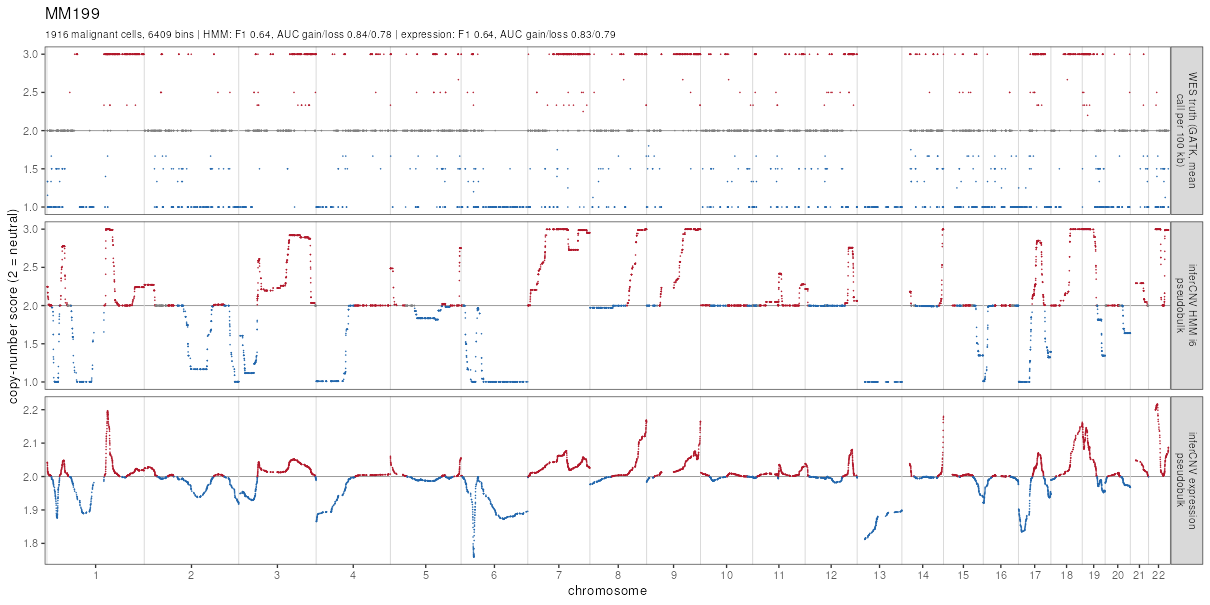
\includegraphics[width=\textwidth]{figures/fig4_MM199_genome.png}
\caption{\textbf{Comparison with DNA-based copy number in multiple myeloma MM199 (10x).} Top, whole-exome copy number segments (Schmid et al.~truth). Below, inferCNV pseudobulk scores over 1,916 malignant cells: HMM states after Bayesian filtering (CNV score) and final residual expression (expression score), in 100-kb bins along the genome. \todo{Panel with ROC curves and metric summary, if wanted; RESULT PENDING: BCH869 panel against WGS clone copy number.} Settings as in Methods.}
\label{fig:4}
\end{figure}

\begin{figure}[p]
\centering
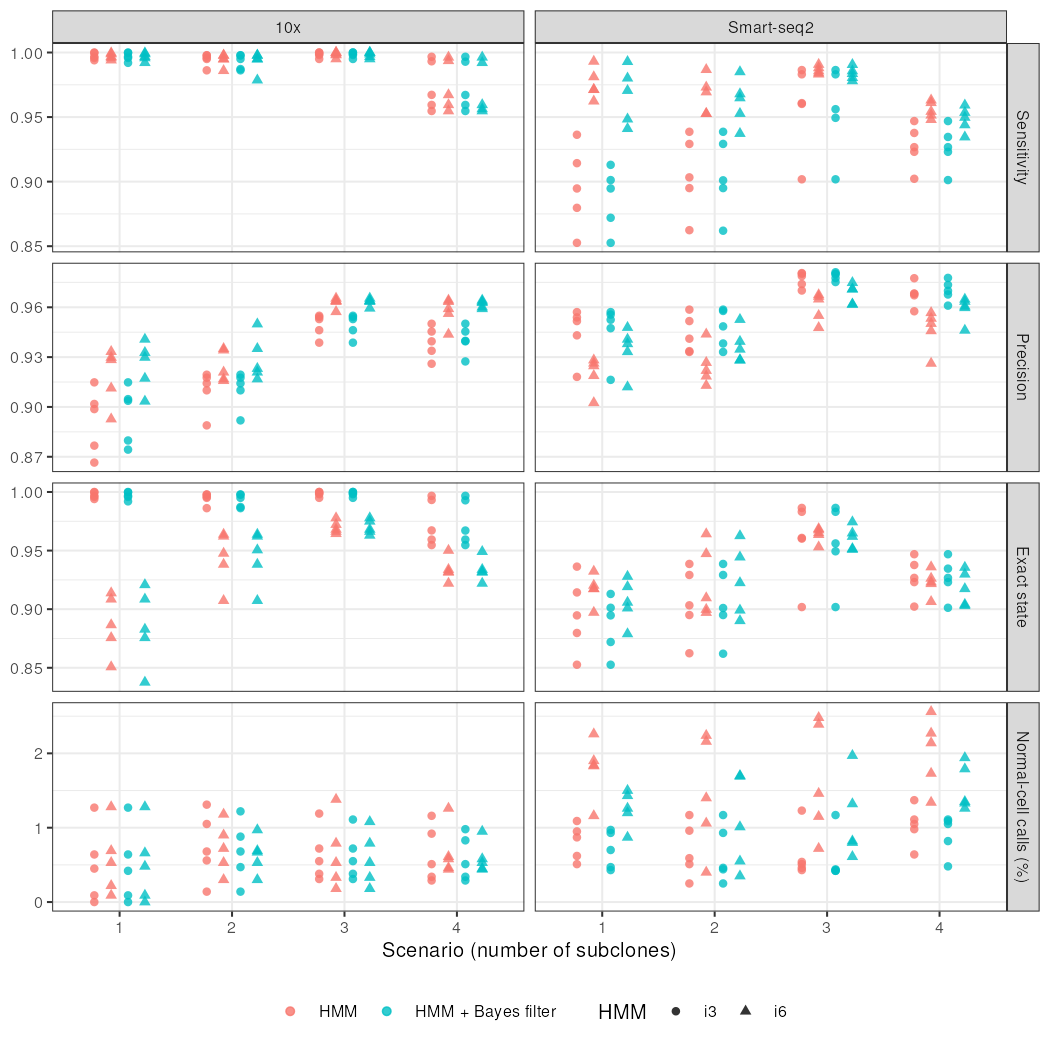
\includegraphics[width=\textwidth]{figures/fig5_simulation.png}
\caption{\textbf{Accuracy on simulated tumours.} Sensitivity, precision, exact-state accuracy, reference call rate and subcluster purity of the i6 HMM after Bayesian filtering for simulated 10x and Smart-seq2 data with one to four subclones (sim1--sim4), over five seeds (points) with means (bars); values in Table 1. \todo{Optional inset: i3 against i6.} \todo{Figure drawn from analyses/simulation/fig5\_simulation.png; check that it shows the master-build numbers of Table 1.}}
\label{fig:5}
\end{figure}

\begin{figure}[p]
\centering
\fbox{\parbox[c][4cm][c]{0.9\textwidth}{\centering Figure 6 pending}}
\caption{\textbf{Specificity and scale.} \todo{RESULT PENDING} (a) Non-neutral call rate in PBMC from healthy donors, by cell type, before and after Bayesian filtering. (b) Run time and peak memory against number of cells, with and without the Bayesian model and for i6 and i3.}
\label{fig:6}
\end{figure}

\begin{figure}[p]
\centering
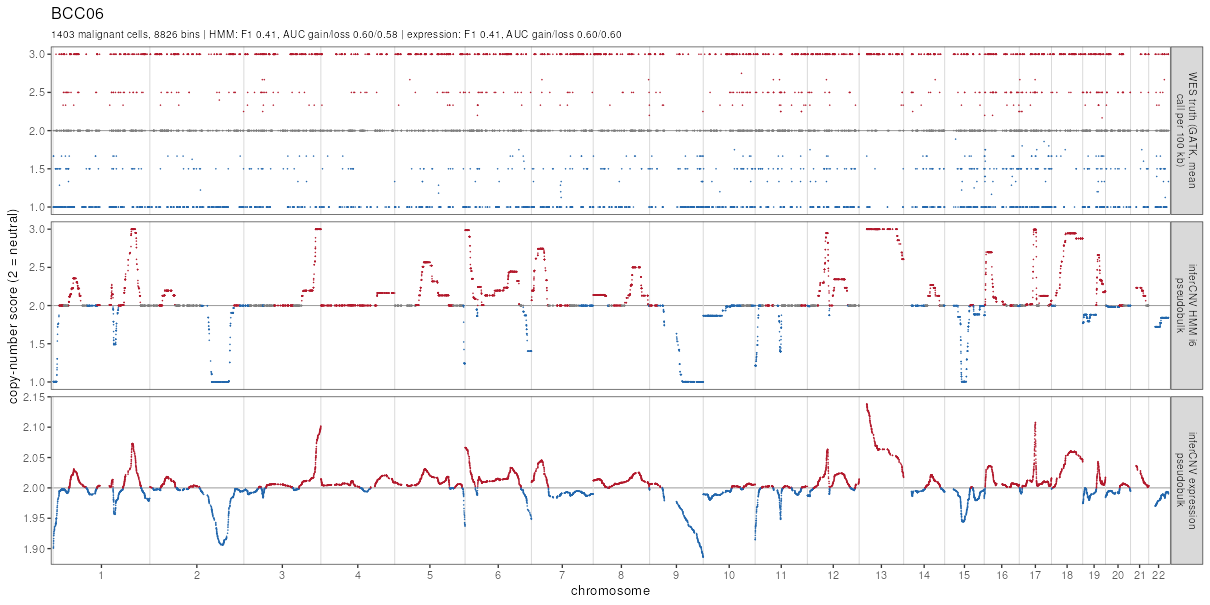
\includegraphics[width=\textwidth]{figures/figS1_BCC06_genome.png}
\caption{\textbf{Basal cell carcinoma BCC06 before and after treatment.} As Fig. 4, for BCC06 (1,403 malignant and 33 reference cells) and BCC06post (320 malignant and 280 reference cells). The exome segmentation of these samples is highly fragmented; see text.}
\label{fig:S1}
\end{figure}

% Supplementary Table S2: Metrics against DNA-based copy number.
% For each sample and score: number of malignant cells and bins, maximal F1, sensitivity and precision for gains and losses at the optimum, AUC and partial AUC for gains and losses, Pearson r; with the values reported by Schmid et al.~for inferCNV v1.10. (From analyses/fig4/metrics\_fig4.tsv and schmid2025\_reported\_infercnv\_v1.10.tsv.)
               -> figure
% The figure is emitted by the macro, not at \input time, so that it is numbered after the
% other supplementary figures.
%
% Everything below was derived from the release code (branch allele_integration):
% R/inferCNV_hidden_spike.R, R/inferCNV_meanVarSim.R, R/inferCNV_simple_sim.R (dropout fit),
% R/inferCNV_HMM.R, R/inferCNV_i3HMM.R, R/inferCNV_BayesNet.R, inst/BUGS_Mixture_Model{,_i3};
% allele-aware: R/inferCNV_allele.R, R/inferCNV_allele_HMM.R, R/inferCNV_allele_native.R,
% R/inferCNV_allele_BayesNet.R, R/inferCNV_combined_BayesNet.R. HoneyBADGER comparison: notes/honeybadger_lineage.md.

\subsection*{Generative models of the expression track: h-spike simulation, hidden Markov models and Bayesian mixture}
\label{sec:supp_models}

This section gives the models of steps 3, 19 and 20--21 in full (Supplementary Fig.~\ref{fig:Smodels}). Throughout, $x_{ij}$ is the residual expression of gene $i$ (in genomic order) in cell $j$ after step 16 (and step 18, if outlier pruning is on), on the fold-change scale with 1 as neutral; this is the matrix on which the HMM and the Bayesian model operate. A cell group $c$ (a subcluster by default, or an annotation group, or a single cell) has $n_c$ cells and mean residual $\bar x_{ic} = n_c^{-1}\sum_{j\in c} x_{ij}$. The i6 states $k=1,\dots,6$ correspond to the simulated levels $c_k\in\{0.01, 0.5, 1, 1.5, 2, 3\}$ (0 to $\geq$5 copies; $k=3$ neutral); the i3 states to loss, neutral and gain ($k=2$ neutral).

\paragraph{h-spike simulation (step 3, i6 only).}
Let $y_{ij}$ be the depth-normalised counts of step 3. For every annotation group $a$ (each observation group and each reference group) and gene $i$, the mean $m_{ia}$, variance $v_{ia}$ and zero fraction $p^0_{ia}$ over the group's cells are computed, and two smoothing splines (\texttt{smooth.spline}, smoothing parameter by generalised cross-validation) are fitted over all (gene, group) pairs: $f_v$ to $\log(v_{ia}+1)$ against $\log(m_{ia}+1)$, and $f_0$ to $p^0_{ia}$ against $\log m_{ia}$ (genes with $m_{ia}>0$). Both trends are thus estimated from all cells, observations included; only the gene means come from the reference cells. The synthetic genome has 11 chromosomes with copy factors $c_r = (1, 0.01, 1, 0.5, 1, 1.5, 1, 2, 1, 3, 1)$; the first ten have 400 genes each and the last $\max(G-4000, 400)$, where $G$ is the number of genes in the data, so that $G'=G$ genes whenever $G\geq 4400$. For each reference group $g$ (or the pooled references with \texttt{hspike\_aggregate\_normals}; all observations when there is no reference), each synthetic gene $i$ receives the mean of a data gene $\pi(i)$ drawn uniformly with replacement, $\tilde m_i = \max(m_{\pi(i) g}, 10^{-3})$, with the same $\pi$ for every group. Two sets of 100 cells are simulated, normal ($t=\mathrm{no}$) with $\mu^{(\mathrm{no})}_i=\tilde m_i$ and spiked ($t=\mathrm{sp}$) with $\mu^{(\mathrm{sp})}_i = c_{r(i)}\tilde m_i$. Counts are drawn independently for each gene and cell as a rounded, truncated normal with the variance predicted by the spline,
\begin{equation}
\tilde y_{ij} = \mathrm{round}\big(\max\{\,\mathcal N(\mu_i, s_i^2),\,0\}\big),\qquad
s_i^2 = \max\{\exp f_v(\log(\mu_i+1)) - 1,\ 0\},
\end{equation}
and dropout is then imposed per gene so that the zero fraction matches the trend: with $\pi_i = f_0(\log \bar{\tilde y}_{i\cdot})$ the predicted zero fraction at the simulated gene mean and $z_i$ the number of zeros already present among the $n=100$ cells, each nonzero $\tilde y_{ij}$ is set to zero independently with probability $\rho_i = \max\{(n\pi_i - z_i)/(n - z_i),\,0\}$. The resulting matrix $y^{\mathrm h}$ (200 cells per reference group) is depth-normalised to the median library size of the data and then carried through steps 6--16 in parallel with the data, with the simulated normal cells serving as the h-spike's own reference groups (it is not subclustered). The emission parameters of level $k$ are the mean and standard deviation of the pooled processed residuals $x^{\mathrm h}_{ij}$ of the spiked cells on the chromosomes with $c_r=c_k$ (the six neutral chromosomes are pooled for $k=3$):
\begin{equation}
\mu_k = \mathrm{mean}(P_k),\quad \sigma_k = \mathrm{sd}(P_k),\qquad P_k=\{x^{\mathrm h}_{ij}:\ c_{r(i)}=c_k,\ j\ \text{spiked}\}.
\end{equation}
To obtain the spread of a mean over $n$ cells, for $n=1,\dots,100$ the standard deviation $\hat\sigma_k(n)$ of the mean of $n$ values drawn with replacement from $P_k$ is estimated over 100 rounds (the $n=1$ point is undefined and dropped), and a line is fitted by least squares,
\begin{equation}
\log\hat\sigma_k(n) = a_k + b_k\log n,\qquad \sigma_k(n_c) = \exp(a_k + b_k\log n_c),
\end{equation}
with $b_k\approx-\tfrac12$ (Fig.~\ref{fig:2}f). The means $\mu_k$ are not scaled. In \texttt{analysis\_mode = "cells"} the single-cell $\sigma_k$ is used directly.

\paragraph{Hidden Markov model (step 19).}
For each chromosome with genes $i=1,\dots,L$ and each cell group $c$, the hidden states $s_i\in\{1,\dots,K\}$ ($K=6$ or 3) form a Markov chain with initial distribution $\delta$ and transition matrix $A$,
\begin{equation}
\Pr(s_1=k)=\delta_k,\qquad \Pr(s_{i+1}=l\mid s_i=k)=A_{kl},\qquad A_{kk}=1-(K-1)t,\quad A_{kl}=t\ (k\neq l),
\end{equation}
with $t=$ \texttt{HMM\_transition\_prob} $=10^{-6}$ and $\delta$ equal to $1-(K-1)t$ for the neutral state and $t$ otherwise. The emission model is Gaussian, $\bar x_{ic}\mid s_i=k \sim \mathcal N(\mu_k, \sigma_k(n_c)^2)$. For i6, $\mu_k$ and $\sigma_k(n_c)$ are the h-spike values above. For i3, with $R$ the set of residuals $x_{ij}$ of all reference cells (all cells when there is no reference), $\mu=\mathrm{mean}(R)$ and $\sigma=\mathrm{sd}(R)$ define the neutral state, the loss and gain means are $\mu\mp\Delta$ with
\begin{equation}
\Delta = \sigma\,\Phi^{-1}(1-p),\qquad p=\texttt{HMM\_i3\_pval}=0.05\ \ (\Delta = 1.645\,\sigma),
\end{equation}
and all three states share $\sigma$, which is not scaled with $n_c$. With \texttt{HMM\_i3\_use\_KS}, $\Delta$ is instead taken from a straight-line fit of the shift $d\in\{0,\sigma/10,\dots,\sigma\}$ on the mean two-sample Kolmogorov--Smirnov $p$-value (100 replicates) between $n_R$ draws from $\mathcal N(0,\sigma^2)$ and $n_R$ draws from $\mathcal N(d,\sigma^2)$, evaluated at $p$, where $n_R$ is the number of reference cells. The i3 model is the expression HMM of HoneyBADGER \citep{fan2018}, which has the same three states, the same transition probability and a common standard deviation; HoneyBADGER places the loss and gain means at a fixed $\mp m$ ($m=0.15$ by default) and takes the standard deviation from the group's mean profile, and the Kolmogorov--Smirnov calibration is its procedure (\texttt{setGexpDev}, with 101 draws per sample rather than $n_R$). HoneyBADGER runs the HMM on the groups obtained by cutting a hierarchical clustering of the cells at successive heights; inferCNV runs it on its subclusters.

The chain is decoded by the Viterbi algorithm. HoneyBADGER uses the standard algorithm of the HiddenMarkov package; the inferCNV implementation (\texttt{Viterbi.dthmm.adj}, adapted from the HiddenMarkov package \citep{hiddenmarkov}) departs from the textbook recursion in the emission term: the state standard deviations are replaced by their median, $\tilde\sigma_c = \mathrm{median}_k\,\sigma_k(n_c)$ (for i3, $\tilde\sigma_c=\sigma$), and the Gaussian density is replaced by a normalised score based on the one-sided tail probability of each state,
\begin{equation}
q_{ik} = 1-\Phi\!\left(\frac{|\bar x_{ic}-\mu_k|}{\tilde\sigma_c}\right),\qquad
b_{ik} = \frac{(-\log q_{ik})^{-1}}{\sum_{l=1}^{K}(-\log q_{il})^{-1}},
\label{eq:emission}
\end{equation}
so that $b_{ik}$ is the relative, not absolute, support for state $k$ at gene $i$ and decays more slowly with distance from $\mu_k$ than a Gaussian. The recursion is $\nu_{1k} = \log\delta_k + \log b_{1k}$, $\nu_{ik} = \max_l\{\nu_{i-1,l} + \log A_{lk}\} + \log b_{ik}$, with the usual back-trace $\hat s_L=\arg\max_k \nu_{Lk}$ and $\hat s_i = \arg\max_k\{\nu_{ik}+\log A_{k\hat s_{i+1}}\}$. A chromosome with a single gene is assigned the neutral state. All cells of the group receive the group's state sequence; a region is a maximal run of consecutive genes of a chromosome with the same state in a group, and the states are mapped to the representative values 0, 0.5, 1, 1.5, 2, 3 (i6) or 0.5, 1, 1.5 (i3) for output.

\paragraph{Bayesian latent mixture model (steps 20--21).}
Re-examining each HMM region with a Bayesian model of its cells is HoneyBADGER's approach \citep{fan2018}: there, each cell of a region is either unaltered or altered, with one direction of change per region and a change of fixed magnitude, and the model is fitted in JAGS. inferCNV generalises it to a mixture over all $K$ HMM states. Each HMM region $r$ with genes $G_r$, called in cell group $c$, is modelled with the cells $C_r$ of that group ($|C_r|=n_c$) as a finite mixture of the $K$ state distributions with known components (model files \texttt{inst/BUGS\_Mixture\_Model} for i6 and \texttt{inst/BUGS\_Mixture\_Model\_i3} for i3):
\begin{equation}
\theta \sim \mathrm{Dirichlet}(1,\dots,1),\qquad
\varepsilon_j \mid \theta \sim \mathrm{Categorical}(\theta),\qquad
x_{ij}\mid \varepsilon_j=k \sim \mathcal N(\mu_k, \tau_k^{-1}),\quad i\in G_r,\ j\in C_r,
\end{equation}
with the state means $\mu_k$ and precisions $\tau_k=\sigma_k^{-2}$ fixed: for i6 the single-cell h-spike values ($\sigma_k$, not $\sigma_k(n_c)$, because the model describes individual cells), and for i3 the means $\mu-\Delta,\mu,\mu+\Delta$ with common precision $\sigma^{-2}$, where $\Delta$ is always the $p$-value shift ($\texttt{HMM\_i3\_use\_KS}$ affects only the HMM). Genes within a cell are conditionally independent given the cell's state, and residuals are assumed independent across cells (Supplementary Fig.~\ref{fig:Smodels}d).

Both full conditionals have closed forms. Given the states, the mixing proportions are $\theta\mid\varepsilon \sim \mathrm{Dirichlet}(1+n_1,\dots,1+n_K)$ with $n_k=\#\{j:\varepsilon_j=k\}$; given $\theta$, each cell's state has $\Pr(\varepsilon_j=k\mid\theta,x)\propto\theta_k\prod_{i\in G_r}\mathcal N(x_{ij};\mu_k,\tau_k^{-1})$, which depends on the data only through $\sum_i x_{ij}$ and $\sum_i x_{ij}^2$. Gibbs sampling alternates the two. The released code did this in JAGS \citep{plummer2003jags} through rjags \citep{rjags}; inferCNV now draws the same two conditionals directly in R (option \texttt{infercnv.bayes\_sampler = "native"}, the default; \texttt{"jags"} restores JAGS, which is also used for a user-supplied model file). $K$ chains are run, chain $k$ initialised with every cell in state $k$; 700 iterations are discarded (JAGS: 500 adaptation and 200 burn-in iterations; adaptation has no effect on these exact updates) and 1,000 are retained from each chain, and the $K\times 1{,}000$ draws are pooled. The chains are drawn together as one vectorised computation from R's generator, so that a run with \texttt{seed} set is reproducible. On the TNBC1 data, the posterior probabilities of the neutral state from the R sampler and from JAGS agreed closely over the 1,913 regions (Pearson $r=0.99993$; largest difference 0.0096), 1,912 filtering decisions were identical (the remaining region had probabilities of 0.499 and 0.501), and on four threads the sampling took 3 instead of 49 minutes (8.8 instead of 55 minutes with the posterior summaries).

The region-level posterior probability of state $k$ is the posterior mean of the mixing proportion, $P_r(k)=\mathbb E[\theta_k\mid x]$, and the cell-level probability $P_{rj}(k)=\Pr(\varepsilon_j=k\mid x)$ is the fraction of draws in which cell $j$ is in state $k$. Because the components are fixed, $P_r(k)\approx(\bar n_k+1)/(n_c+K)$, where $\bar n_k$ is the posterior mean number of cells in state $k$: it is essentially the fraction of the group's cells whose residuals over $G_r$ are best explained by state $k$, shrunk towards $1/K$ by the prior. (One consequence is that with i6 a region in a group of four or fewer cells cannot reach $P_r(\text{neutral})>0.5$ even if every cell looks neutral.) The residuals are smoothed over about 100 genes, so neighbouring genes of a cell are strongly correlated, whereas the model multiplies their likelihoods as if they were independent. The per-cell posteriors are therefore over-confident, usually close to 0 or 1, and are better read as hard assignments than as calibrated probabilities; $P_r(k)$ is affected less, because it depends mainly on how many cells are assigned to each state. Filtering (step 21) resets a region to neutral when $P_r(\text{neutral})>$ \texttt{BayesMaxPNormal}; otherwise, with \texttt{reassignCNVs}, its state becomes $\arg\max_k P_r(k)$, which can itself be the neutral state. The cell-level probabilities are plotted and stored in the output object, but are not used for filtering.

\subsection*{Allele-aware models}
\label{sec:supp_allele}

When allele counts are supplied, inferCNV adds the allelic imbalance of heterozygous single-nucleotide polymorphisms (SNPs) to the expression signal (steps 2, 4--5 and 23--28; Supplementary Fig.~\ref{fig:Sallele}). Allelic imbalance shows events that expression cannot: copy-neutral loss of heterozygosity (LOH), and which kind of change underlies an expression shift. The extension, written by Yu Zhong, follows HoneyBADGER \citep{fan2018} closely. Its allele HMM is HoneyBADGER's, and the allele-only and combined Bayesian models of the release were ports of HoneyBADGER's allele model and joint expression--allele model, extended to the inferCNV states. For this paper we revised the two Bayesian models; they are described below, followed by the changes from the release. The data preparation, the allele HMM and the fusion of expression and allele segments are as released.

\paragraph{Allele data (steps 2, 4 and 5).}
\texttt{CreateInfercnvObject()} takes, besides the expression counts, two SNP $\times$ cell matrices: the alternative-allele read counts (\texttt{raw\_allele\_matrix}) and the total read counts (\texttt{raw\_coverage\_matrix}), with SNPs named by chromosome and position. In step 2, a SNP is kept as heterozygous if at least \texttt{min\_cells\_per\_snp} (default 3) reference cells have an alternative-allele fraction below 0.5 and at least as many have one above 0.5 (all cells are used when there is no reference). Entries with coverage below \texttt{snp\_min\_coverage} (default 0, i.e.\ off) are set to zero. For each SNP, the counts are then re-expressed as those of its \emph{lesser} allele, the allele that is in the minority in most of the observation cells that cover it; inferCNV thus needs no phasing. HoneyBADGER orients each SNP in the same way, from the allele fraction of a bulk or pooled ``in-silico bulk'' sample. Below, $r_{sj}$ is the lesser-allele count and $n_{sj}$ the total count of SNP $s$ in cell $j$. In step 4 each SNP is assigned to the nearest gene of the gene order file, including SNPs between genes. With \texttt{allele\_mode = "gene\_level"}, step 5 keeps, for each gene and cell, the SNP with the highest coverage (\texttt{collapse\_method = "highest"}), so that the models below run on one value per gene; the default, \texttt{"snp\_level"}, keeps all SNPs.

\paragraph{Allele HMM (step 23).}
For each subcluster $c$ with at least two cells and each chromosome, the allele HMM segments the SNPs, in genomic order, into allelically imbalanced and balanced stretches (Supplementary Fig.~\ref{fig:Sallele}a). The observation at SNP $s$ is the number of the subcluster's cells that show the lesser allele at all, $m_{sc}=\#\{j\in c: r_{sj}>0\}$, out of the number of cells that cover the SNP, $N_{sc}=\#\{j\in c: n_{sj}>0\}$. With one or two reads per cell, as is typical, a covered cell of a balanced region shows the lesser allele about half the time, whereas in a region that has lost one allele it shows it only through errors or contaminating cells. The two hidden states $z_s$ therefore have emissions
\begin{equation}
m_{sc}\mid z_s \sim \mathrm{Binomial}(N_{sc}, p_{z_s}),\qquad p_{\mathrm{imbalanced}} = 0.1,\quad p_{\mathrm{balanced}}=0.45,
\end{equation}
with transition probability $t=10^{-6}$ and initial probabilities $(\tfrac12,\tfrac12)$. The chain is decoded by the Viterbi algorithm, with the binomial probabilities floored at $t$ and normalised over the two states. Runs of at least five consecutive imbalanced SNPs are kept, and every SNP within the genomic span of a kept run is marked imbalanced for the cells of the subcluster. The model and all its constants are those of HoneyBADGER's \texttt{calcAlleleCnvBoundaries}. HoneyBADGER also trims 10\% of the SNPs from each run and runs the HMM on groups from successive cuts of a hierarchical clustering; inferCNV does not trim and uses its subclusters.

\paragraph{Allele-only Bayesian model (steps 24--25).}
As for expression, each allele-HMM region $r$, with SNPs $S_r$ and the cells $C_r$ of the subcluster in which it was called, is re-examined with a mixture model over its cells (Supplementary Fig.~\ref{fig:Sallele}b). Each cell is either allelically imbalanced or balanced, $\varepsilon_j\mid\theta\sim\mathrm{Categorical}(\theta)$ with $\theta\sim\mathrm{Dirichlet}(1,1)$. Each state is a set of genotypes with an expected lesser-allele fraction $f$. The imbalanced state covers the genotypes that lose one allele (one-copy loss or copy-neutral LOH; $f=\epsilon=0.01$, allowing for errors) and those that gain one (three copies, $f=\tfrac13$; four copies split 3:1, $f=\tfrac14$), each with equal prior weight; the balanced state has $f=\tfrac12$. Write $f_j$ for the fraction of the genotype of cell $j$. The lesser allele of step 2 is defined over all tumour cells and need not be the allele reduced in this subclone, so each SNP of the region has a latent orientation $a_s\sim\mathrm{Bernoulli}(\tfrac12)$, shared by all cells of the region:
\begin{equation}
p_{sj} = a_s f_j + (1-a_s)(1-f_j),\qquad
r_{sj}\mid n_{sj} \sim \mathrm{BetaBinomial}\big(n_{sj},\ \kappa p_{sj},\ \kappa(1-p_{sj})\big),
\end{equation}
over the SNP--cell pairs with coverage. Because the orientation is shared, imbalance must favour the same allele of each SNP in every cell of the state, which separates a genomic loss from random monoallelic expression of individual cells. The beta-binomial allows the reads of a cell at a SNP to be more variable than independent draws, as transcriptional bursting and other sources of allelic overdispersion make them; it has mean $p_{sj}$ and concentration $\kappa$. $\kappa$ is fitted once per run by maximum likelihood over all covered SNP--cell pairs of the reference cells with $p=\tfrac12$, where heterozygous SNPs are balanced (on the TNBC1 data, $\kappa=21.7$ from 302 reference cells). When the reference cells have fewer than 50 covered pairs, for example when they come from another sample without allele data, $\kappa$ is fitted on all cells with each SNP's mean set to its pooled lesser-allele fraction (clipped to $[0.01, 0.99]$), so that imbalance from CNAs is not mistaken for overdispersion; with fewer than 50 pairs in all, $\kappa=10$. In step 25, a region is reset to balanced when $P_r(\text{balanced})>$ \texttt{BayesMaxPNormal}, and kept as imbalanced otherwise. With \texttt{allele\_mode = "gene\_level"}, $s$ runs over the region's genes, each with the counts of its chosen SNP.

\paragraph{Fusion of expression and allele segments (step 26).}
For each subcluster, the regions remaining after the expression filter (step 21) and the allele filter (step 25) are cut into disjoint segments. Each segment takes the expression state of the region that covers it (neutral if none) and the allele state (balanced if none). The segment's combined state is the expression state, except that allelic imbalance with neutral expression becomes copy-neutral LOH (state 7 with i6, 4 with i3), and allelic imbalance with a 0-copy expression state, which is contradictory because no allele is expressed, is flagged as state 8 (i6). Each gene takes the state of the first segment it overlaps. With \texttt{combined\_method = "common"} instead of the default \texttt{"union"}, only genes with SNPs are kept. In the release, the fusion read the unfiltered HMM reports of steps 19 and 23, so the two filters had no effect on the combined result.

\paragraph{Combined expression and allele model (steps 27--28).}
Each fused region $r$, with genes $G_r$, the SNPs $S_r$ assigned to those genes and the cells $C_r$ of its subcluster, is fitted with a mixture over copy-number states in which each cell's state must explain both its expression and its alleles (Supplementary Fig.~\ref{fig:Sallele}c). HoneyBADGER's joint model has the same structure, with one cell-level indicator of an altered state; here the states are those of the HMM plus copy-neutral LOH: for i6, 0, 1, 2, 3, 4 and $\geq$5 copies and copy-neutral LOH; for i3, loss, neutral, gain and copy-neutral LOH. Each state has genotypes with lesser-allele fractions $f$:
\begin{center}
\small
\begin{tabular}{lll}
\hline
i6 state & genotypes & $f$\\
\hline
0 copies & -- & $\tfrac12$ (no allelic information; reads are ambient or from other cells)\\
1 copy & (1,0) & $\epsilon$\\
2 copies & (1,1) & $\tfrac12$\\
3 copies & (2,1) & $\tfrac13$\\
4 copies & (2,2), (3,1) & $\tfrac12$, $\tfrac14$\\
$\geq$5 copies & e.g.\ (3,3), (4,2), (5,1) & $\tfrac12$, $\tfrac13$, $\tfrac16$\\
copy-neutral LOH & (2,0) & $\epsilon$\\
\hline
\end{tabular}
\end{center}
For i3, loss has $f=\epsilon$, neutral $f=\tfrac12$, gain $f\in\{\tfrac12,\tfrac13,\tfrac14\}$ and copy-neutral LOH $f=\epsilon$. The genotypes of a state have equal prior weight. The allele likelihood, the orientations $a_s$ and $\kappa$ are as in the allele-only model. For expression, the model uses each cell's mean residual over the region, $\bar x_j = |G_r|^{-1}\sum_{i\in G_r}x_{ij}$:
\begin{equation}
\bar x_j\mid \varepsilon_j=k \sim \mathcal N\!\left(\mu_k,\ \big(s_r\,\sigma_k/\sigma_{\mathrm{neutral}}\big)^2\right),
\end{equation}
where $\mu_k$ and $\sigma_k$ are the single-cell state means and standard deviations of the expression model (h-spike for i6, reference residuals for i3), copy-neutral LOH takes the neutral values, and $s_r$ is the standard deviation of the same region mean across the reference cells (the single-cell $\sigma_{\mathrm{neutral}}$ when there are fewer than five). Smoothing makes neighbouring genes nearly identical, so the per-gene likelihood of the expression-only model would count the expression evidence of a large region many times over and swamp the alleles; the region mean, with its spread measured on reference cells, gives expression the weight it actually has. A region without SNPs is fitted with the expression term alone and without the copy-neutral LOH state. In step 28 a region is reset to neutral when $P_r(\text{neutral})>$ \texttt{BayesMaxPNormal}; otherwise it takes its most probable state, which may be copy-neutral LOH.

\paragraph{Sampling.}
Both allele-aware models are fitted by Gibbs sampling in R. Each sweep draws, for every cell, its state and genotype jointly from their categorical full conditional given $\theta$ and the orientations; then $\theta$ from its Dirichlet full conditional; then each orientation $a_s$ from its Bernoulli full conditional, whose log-odds are the summed differences, over the cells of a non-balanced genotype, between the beta-binomial log-likelihoods of $r_{sj}$ at $f_j$ and at $1-f_j$. One chain is run per state, initialised with all cells in that state and all $a_s=1$, with 700 iterations discarded and 1,000 retained. The per-SNP likelihood terms are computed once per region, so a sweep costs time proportional to the number of covered SNP--cell pairs. On simulated regions with 10x-like and Smart-seq2-like coverage, the combined model assigned neutral, one-copy loss, three-copy gain and copy-neutral LOH regions to the correct state.

\paragraph{Changes from the release.}
The release fitted ports of HoneyBADGER's BUGS models in JAGS. In the allele-only model, a balanced cell had, for every gene, either a SNP-specific allele probability with a nearly flat prior (truncated $\mathcal N(0.5, \text{precision } 0.1)$ on $[0.1, 0.9]$) or, with prior probability 0.7, monoallelic expression in a random direction; an imbalanced cell had a lesser-allele probability of 0.1. A ``bulk'' binomial term determined the orientation of each SNP. In HoneyBADGER the bulk counts come from a separate bulk sample or from all cells; in the release they were recomputed from the cells being modelled, so that the same reads entered twice. The combined model extended this to the i6 or i3 states with an added copy-neutral LOH state. Only the 1-copy and copy-neutral LOH states were imbalanced, so an imbalanced gain (for example 2:1) could be explained by the alleles only as LOH. Each gene's expression residual entered as an independent observation. The revised models replace the per-gene allele model with the beta-binomial, fitted on reference cells, and the bulk term with the shared orientations $a_s$, which play the same part. They give the gain states their imbalanced genotypes, and use the region mean for expression. The release versions remain available with \texttt{options(infercnv.bayes\_sampler = "jags")}.

% ------------------------------------------------------------------
% The figure. Emitted where \SuppModelsFigure is called (after sections/figures.tex).
% TikZ bodies of the model diagrams (Supplementary Fig. \ref{fig:Smodels}).
% Shared by sections/supp_models.tex (via \SuppModelsFigure) and figures/plates_standalone.tex.
% Requires: \usepackage{tikz} \usetikzlibrary{bayesnet,positioning,fit,arrows,calc}
%
% Node conventions (tikz-bayesnet): latent = white circle (random), obs = grey circle
% (observed / given data), det = diamond (deterministic function of its parents),
% const = plain text (fixed quantity). Plates = replication.

\tikzset{
  mnode/.style={font=\footnotesize},
  plate caption/.append style={font=\scriptsize},
  note/.style={font=\scriptsize, text=black!70, align=left, inner sep=1pt},
  >=stealth,
}

% ------------------------------------------------------------------
% (a) h-spike simulator (one reference group g)
% ------------------------------------------------------------------
\newcommand{\PlateHspike}{%
\begin{tikzpicture}[node distance=0.5cm and 0.7cm, mnode]
  % given data and the quantities derived from it
  \node[obs]                                  (Y)  {$y$};
  \node[note, above=0.05cm of Y, align=center] {depth-normalised counts,\\all annotation groups};
  \node[det, below=0.5cm of Y] (m)  {$m_g$};
  \node[note, right=0.05cm of m] {gene means,\\ref.\ group $g$};
  \edge{Y}{m};
  % genes plate
  \node[det, below=0.7cm of m]          (mt)  {$\tilde m_i$};
  \node[const, right=0.7cm of mt]       (c)   {$c_{r(i)}$};
  \node[det, below=of mt]               (mu)  {$\mu^{(t)}_i$};
  \node[latent, below=0.6cm of mu]      (yt)  {$\tilde y_{ij}$};
  \node[latent, below=0.6cm of yt]      (yd)  {$y^{\mathrm h}_{ij}$};
  \edge{m}{mt}; \edge{mt}{mu}; \edge{c}{mu}; \edge{mu}{yt}; \edge{yt}{yd};
  \plate[inner sep=0.16cm]{cells}{(yt)(yd)}{$j=1,\dots,100$}
  \plate[inner sep=0.22cm]{type}{(cells)}{$t\in\{\mathrm{no},\mathrm{sp}\}$}
  \plate[inner sep=0.26cm]{genes}{(mt)(c)(mu)(type)}{$i=1,\dots,G'$}
  % splines, outside the plates, feeding the simulated counts
  \node[det, left=1.6cm of yt] (fv) {$f_v$};
  \node[det, left=1.6cm of yd] (f0) {$f_0$};
  \node[note, left=0.05cm of fv, align=right] {mean--variance\\spline};
  \node[note, left=0.05cm of f0, align=right] {mean--dropout\\spline};
  % edges from the data run left at the height of y, then down (right of the spline nodes)
  \draw[->] (Y.west) -| (fv.north);
  \draw[->] (Y.west) -| ($(f0.north east)+(0.25,0.35)$) -- (f0.north east);
  \edge{fv}{yt}; \edge{f0}{yd};
  % downstream
  \node[det, below=0.8cm of genes] (x) {$x^{\mathrm h}_{ij}$};
  \node[note, right=0.1cm of x] {residuals after steps 6--16,\\mirrored on the h-spike};
  \draw[->] (genes.south) -- (x);
  \node[const, below=0.45cm of x] (par) {$\mu_k,\ \sigma_k,\ \sigma_k(n)$};
  \node[note, right=0.1cm of par] {per level $k$, from the spiked cells\\of the chromosomes with $c_r=c_k$};
  \edge{x}{par};
\end{tikzpicture}}

% ------------------------------------------------------------------
% HMM chain on one chromosome of one cell group c (shared by the i6 and i3 diagrams)
% ------------------------------------------------------------------
\newcommand{\HMMchain}{%
  \node[const]                          (delta) {$\delta$};
  \node[latent, below=0.5cm of delta]   (s1) {$s_1$};
  \node[latent, below=of s1]            (s2) {$s_2$};
  \node[latent, below=of s2]            (s3) {$s_3$};
  \node[below=0.2cm of s3]              (dots) {$\vdots$};
  \node[latent, below=0.2cm of dots]    (sL) {$s_L$};
  \node[obs, right=of s1] (x1) {$\bar x_{1c}$};
  \node[obs, right=of s2] (x2) {$\bar x_{2c}$};
  \node[obs, right=of s3] (x3) {$\bar x_{3c}$};
  \node[obs, right=of sL] (xL) {$\bar x_{Lc}$};
  \edge{delta}{s1}; \edge{s3}{dots}; \edge{dots}{sL};
  \draw[->] (s1) -- node[left, font=\scriptsize] {$A$} (s2);
  \draw[->] (s2) -- node[left, font=\scriptsize] {$A$} (s3);
  \edge{s1}{x1}; \edge{s2}{x2}; \edge{s3}{x3}; \edge{sL}{xL};
  \plate[inner sep=0.2cm]{chr}{(s1)(sL)(x1)(xL)}{$i=1,\dots,L$}}

% ------------------------------------------------------------------
% (b) six-state HMM (i6): emission parameters from the h-spike
% ------------------------------------------------------------------
\newcommand{\PlateHMMsix}{%
\begin{tikzpicture}[node distance=0.45cm and 0.6cm, mnode]
  \HMMchain
  \node[const, right=0.5cm of chr.east, align=center] (par) {$\mu_k$\\$\sigma_k(n_c)$};
  \edge{par}{x1}; \edge{par}{x2}; \edge{par}{x3}; \edge{par}{xL};
  \plate[inner sep=0.26cm]{grp}{(chr)(delta)(par)}{group $c$; chromosomes}
  \node[note, below=0.1cm of grp, text width=4.4cm] {$K=6$ states, $k=3$ neutral; $\mu_k$, $\sigma_k(n_c)$ from the h-spike (a); $\bar x_{ic}$: mean residual of the $n_c$ cells of group $c$ at gene $i$; $A_{kk}=1-5t$, $A_{kl}=t$.};
\end{tikzpicture}}

% ------------------------------------------------------------------
% (c) three-state HMM (i3): emission parameters from the reference residuals
% ------------------------------------------------------------------
\newcommand{\PlateHMMthree}{%
\begin{tikzpicture}[node distance=0.45cm and 0.6cm, mnode]
  \HMMchain
  \node[det, right=0.5cm of chr.east] (par) {$\mu_k,\sigma$};
  \node[det, right=0.5cm of par, yshift=0.9cm]  (mus) {$\mu,\sigma$};
  \node[det, right=0.5cm of par, yshift=-0.9cm] (Del) {$\Delta$};
  \node[obs, above=0.5cm of mus]                (R)   {$R$};
  \node[note, above=0.02cm of R, align=center] {reference\\residuals};
  \node[const, below=0.45cm of Del]             (pv)  {$p$};
  \edge{R}{mus}; \edge{mus}{Del}; \edge{pv}{Del}; \edge{mus}{par}; \edge{Del}{par};
  \edge{par}{x1}; \edge{par}{x2}; \edge{par}{x3}; \edge{par}{xL};
  \plate[inner sep=0.26cm]{grp}{(chr)(delta)}{group $c$; chromosomes}
  \node[note, below=0.1cm of grp, text width=4.6cm] {$K=3$ states (loss, neutral, gain) with means $\mu-\Delta,\ \mu,\ \mu+\Delta$ and common $\sigma$, not scaled with $n_c$; $\Delta=\sigma\Phi^{-1}(1-p)$ or the KS shift; $A_{kk}=1-2t$.};
\end{tikzpicture}}

% ------------------------------------------------------------------
% (d) Bayesian latent mixture model for one HMM region r (i6 and i3)
% ------------------------------------------------------------------
\newcommand{\PlateBayes}{%
\begin{tikzpicture}[node distance=0.5cm and 0.8cm, mnode]
  \node[const]                        (alpha) {$\alpha=(1,\dots,1)$};
  \node[latent, below=0.45cm of alpha] (theta) {$\theta$};
  \node[latent, below=of theta]       (eps)   {$\varepsilon_j$};
  \node[obs, below=of eps]            (x)     {$x_{ij}$};
  \edge{alpha}{theta}; \edge{theta}{eps}; \edge{eps}{x};
  \plate[inner sep=0.16cm]{genes}{(x)}{$i\in G_r$}
  \plate[inner sep=0.24cm]{cells}{(eps)(genes)}{$j\in C_r$}
  \plate[inner sep=0.3cm]{region}{(theta)(cells)}{region $r$}
  % fixed state parameters, shared by all regions
  \node[const, right=1.8cm of x, yshift=0.3cm]  (mu)  {$\mu_k$};
  \node[const, below=0.2cm of mu]               (tau) {$\tau_k$};
  \edge{mu}{x}; \edge{tau}{x};
  \plate[inner sep=0.14cm]{K}{(mu)(tau)}{$K$ states}
  \node[note, below=0.1cm of region, text width=4.4cm] {$\mu_k$, $\tau_k=\sigma_k^{-2}$ fixed (i6: single-cell h-spike values; i3: $\mu\mp\Delta$, $\mu$, $\sigma$). $P_r(k)=\mathbb E[\theta_k\mid x]$, $P_{rj}(k)=\Pr(\varepsilon_j=k\mid x)$.};
\end{tikzpicture}}

% ==================================================================
% Allele-aware models (Supplementary Fig. \ref{fig:Sallele})
% ==================================================================

% ------------------------------------------------------------------
% (a) allele HMM on one chromosome of one subcluster c (step 23)
% ------------------------------------------------------------------
\newcommand{\PlateAlleleHMM}{%
\begin{tikzpicture}[node distance=0.45cm and 0.55cm, mnode]
  \node[const]                          (delta) {$\delta$};
  \node[latent, below=0.5cm of delta]   (z1) {$z_1$};
  \node[latent, below=of z1]            (z2) {$z_2$};
  \node[below=0.2cm of z2]              (dots) {$\vdots$};
  \node[latent, below=0.2cm of dots]    (zL) {$z_L$};
  \node[obs, right=of z1] (m1) {$m_{1c}$};
  \node[obs, right=of z2] (m2) {$m_{2c}$};
  \node[obs, right=of zL] (mL) {$m_{Lc}$};
  \edge{delta}{z1}; \edge{z2}{dots}; \edge{dots}{zL};
  \draw[->] (z1) -- node[left, font=\scriptsize] {$A$} (z2);
  \edge{z1}{m1}; \edge{z2}{m2}; \edge{zL}{mL};
  \node[obs, right=0.45cm of m1] (N1) {$N_{1c}$};
  \node[obs, right=0.45cm of m2] (N2) {$N_{2c}$};
  \node[obs, right=0.45cm of mL] (NL) {$N_{Lc}$};
  \edge{N1}{m1}; \edge{N2}{m2}; \edge{NL}{mL};
  \node[below=0.35cm of mL, inner sep=0pt, minimum size=0pt] (padL) {};
  \plate[inner sep=0.2cm]{chr}{(z1)(zL)(m1)(mL)(N1)(NL)(padL)}{SNPs $s=1,\dots,L$}
  \node[const, right=0.5cm of chr.east] (pp) {$p_{\mathrm{d}},p_{\mathrm{n}}$};
  \coordinate (bus) at ($(chr.east)+(0.2,0)$);
  \draw (pp.west) -- (bus);
  \draw[->] (bus) |- ($(m1.north)+(0,0.3)$) -- (m1.north);
  \draw[->] (bus) |- ($(mL.south)+(0,-0.25)$) -- (mL.south);
  \plate[inner sep=0.26cm]{grp}{(chr)(delta)(pp)}{subcluster $c$; chromosomes}
  \node[note, below=0.1cm of grp, text width=5.0cm] {$z_s\in\{$imbalanced, balanced$\}$; of the $N_{sc}$ cells of $c$ covering SNP $s$, $m_{sc}$ show the lesser allele: $m_{sc}\sim\mathrm{Bin}(N_{sc}, p_{z_s})$, $p_{\mathrm d}=0.1$, $p_{\mathrm n}=0.45$; $A_{kk}=1-t$; $\delta=(\tfrac12,\tfrac12)$.};
\end{tikzpicture}}

% ------------------------------------------------------------------
% (b) allele-only Bayesian mixture for one allele-HMM region r (step 24)
% ------------------------------------------------------------------
\newcommand{\PlateAlleleMix}{%
\begin{tikzpicture}[node distance=0.5cm and 0.6cm, mnode]
  \node[const]                          (alpha) {$\alpha=(1,1)$};
  \node[latent, below=0.4cm of alpha]   (theta) {$\theta$};
  \node[latent, below=of theta]         (eps)   {$\varepsilon_j$};
  \node[latent, below=of eps]           (f)     {$f_j$};
  \node[det, below=0.6cm of f]          (p)     {$p_{sj}$};
  \node[obs, below=0.5cm of p]          (r)     {$r_{sj}$};
  \node[obs, left=0.5cm of r]           (n)     {$n_{sj}$};
  \edge{alpha}{theta}; \edge{theta}{eps}; \edge{eps}{f}; \edge{f}{p}; \edge{p}{r}; \edge{n}{r};
  \plate[inner sep=0.14cm]{snpsin}{(p)(r)(n)}{$s\in S_r$}
  \plate[inner sep=0.22cm]{cells}{(eps)(f)(snpsin)}{$j\in C_r$}
  \node[latent, right=1.3cm of p]       (a)     {$a_s$};
  \plate[inner sep=0.14cm]{snpsout}{(a)}{$s\in S_r$}
  \edge{a}{p};
  \node[const, right=1.3cm of r]        (kap)   {$\kappa$};
  \node[note, below=0.05cm of kap, align=center] {fitted on\\reference cells};
  \edge{kap}{r};
  \plate[inner sep=0.3cm]{region}{(theta)(cells)(snpsout)}{region $r$}
  \node[note, below=0.1cm of region, text width=5.2cm] {$\varepsilon_j\in\{$imbalanced, balanced$\}$; $f_j$: expected lesser-allele fraction of the cell's genotype (imbalanced: $\epsilon$, $\tfrac13$ or $\tfrac14$; balanced: $\tfrac12$); $a_s$: which allele of SNP $s$ is in the minority, shared by all cells; $p_{sj}=f_j$ if $a_s=1$, else $1-f_j$; $r_{sj}\sim\mathrm{BetaBin}(n_{sj},\kappa p_{sj},\kappa(1-p_{sj}))$.};
\end{tikzpicture}}

% ------------------------------------------------------------------
% (c) combined expression + allele Bayesian mixture for one fused region r (step 27)
% ------------------------------------------------------------------
\newcommand{\PlateCombined}{%
\begin{tikzpicture}[node distance=0.5cm and 0.6cm, mnode]
  \node[const]                          (alpha) {$\alpha=(1,\dots,1)$};
  \node[latent, below=0.4cm of alpha]   (theta) {$\theta$};
  \node[latent, below=of theta]         (eps)   {$\varepsilon_j$};
  \node[latent, below=of eps]           (f)     {$f_j$};
  \node[det, below=0.6cm of f]          (p)     {$p_{sj}$};
  \node[obs, below=0.5cm of p]          (r)     {$r_{sj}$};
  \node[obs, left=0.5cm of r]           (n)     {$n_{sj}$};
  \node[obs, left=1.1cm of f]           (x)     {$\bar x_j$};
  \edge{alpha}{theta}; \edge{theta}{eps}; \edge{eps}{f}; \edge{f}{p}; \edge{p}{r}; \edge{n}{r};
  \edge{eps}{x};
  \plate[inner sep=0.14cm]{snpsin}{(p)(r)(n)}{$s\in S_r$}
  \plate[inner sep=0.22cm]{cells}{(eps)(f)(snpsin)(x)}{$j\in C_r$}
  \node[latent, right=1.3cm of p]       (a)     {$a_s$};
  \plate[inner sep=0.14cm]{snpsout}{(a)}{$s\in S_r$}
  \edge{a}{p};
  \node[const, right=1.3cm of r]        (kap)   {$\kappa$};
  \edge{kap}{r};
  \plate[inner sep=0.3cm]{region}{(theta)(cells)(snpsout)}{region $r$}
  % expression parameters
  \node[const, left=1.6cm of x, yshift=0.7cm, align=center] (mu) {$\mu_k,\sigma_k$};
  \node[note, left=0.05cm of mu, align=right] {h-spike (i6) or\\reference (i3)};
  \node[obs, left=1.6cm of x, yshift=-0.9cm] (sref) {$s_r$};
  \node[note, left=0.05cm of sref, align=right] {spread of the\\region mean in\\reference cells};
  \edge{mu}{x}; \edge{sref}{x};
  \node[note, below=0.1cm of region, text width=6.6cm] {$\varepsilon_j$: copy-number state (i6: 0, 1, 2, 3, 4, $\geq$5 copies and copy-neutral LOH; i3: loss, neutral, gain, copy-neutral LOH); $f_j$: lesser-allele fraction of one of the state's genotypes (e.g.\ 3 copies: $\tfrac13$; LOH and 1 copy: $\epsilon$); $\bar x_j$: the cell's mean residual over the region's genes, $\bar x_j\sim\mathcal N\big(\mu_{\varepsilon_j},\,(s_r\sigma_{\varepsilon_j}/\sigma_{\mathrm{neutral}})^2\big)$; allele terms as in b.};
\end{tikzpicture}}

\providecommand{\PlateScale}{0.68}
\newcommand{\SuppModelsFigure}{%
\begin{figure}[p]
\centering
\begin{minipage}[t]{0.49\textwidth}
  \textbf{a}\quad h-spike simulator (i6)\\[2pt]
  \scalebox{\PlateScale}{\PlateHspike}
\end{minipage}\hfill
\begin{minipage}[t]{0.49\textwidth}
  \textbf{b}\quad six-state HMM (i6)\\[2pt]
  \scalebox{\PlateScale}{\PlateHMMsix}
\end{minipage}\\[4pt]
\begin{minipage}[t]{0.49\textwidth}
  \textbf{c}\quad three-state HMM (i3)\\[2pt]
  \scalebox{\PlateScale}{\PlateHMMthree}
\end{minipage}\hfill
\begin{minipage}[t]{0.49\textwidth}
  \textbf{d}\quad Bayesian latent mixture (i6 and i3)\\[2pt]
  \scalebox{\PlateScale}{\PlateBayes}
\end{minipage}
\captionsetup{font={footnotesize,stretch=1}}
\caption{\textbf{Graphical models of the expression track: the i6 calibration, the two HMMs and the Bayesian filter.} Circles are random variables (grey: given data), diamonds deterministic quantities, plain symbols fixed parameters, and boxes replication (plates). \textbf{a}, h-spike simulator (step 3; one reference group $g$): mean--variance and mean--dropout splines ($f_v$, $f_0$) are fitted to the depth-normalised counts $y$, and the reference gene means $m_g$ are sampled to give $\tilde m_i$ on a synthetic genome with copy factors $c_r$; counts of 100 normal and 100 spiked cells are simulated, processed exactly as the data, and their residuals $x^{\mathrm h}_{ij}$ give each level's emission mean $\mu_k$, single-cell standard deviation $\sigma_k$ and group-size scaling $\sigma_k(n)$. \textbf{b}, Six-state HMM for one chromosome of one cell group $c$ (step 19): hidden states $s_i$ with initial distribution $\delta$ and transition matrix $A$ (off-diagonal $t=10^{-6}$), emitting the group's mean residual $\bar x_{ic}$ from $\mathcal N(\mu_k,\sigma_k(n_c)^2)$ with the h-spike parameters of panel a; decoded by Viterbi with the emission score of Eq.~\ref{eq:emission}. \textbf{c}, Three-state HMM, HoneyBADGER's design \citep{fan2018}: the same chain, with the neutral mean $\mu$ and standard deviation $\sigma$ of the reference residuals $R$, loss and gain means $\mu\mp\Delta$ with $\Delta$ set by the tail probability $p$ (or the Kolmogorov--Smirnov criterion), and a standard deviation not scaled with group size. \textbf{d}, Bayesian latent mixture model for one HMM region $r$ (steps 20--21), for either HMM: the cells $C_r$ of the group have states $\varepsilon_j$ drawn from mixing proportions $\theta$ with a flat Dirichlet prior, and the residuals $x_{ij}$ of the region's genes $G_r$ are normal with the fixed mean and precision of the cell's state (i6: single-cell h-spike values; i3: those of panel c). The posterior mean of $\theta$ gives the region's state probabilities, and the posterior of $\varepsilon_j$ the cell-level probabilities.}
\label{fig:Smodels}
\end{figure}}

\newcommand{\SuppAlleleFigure}{%
\begin{figure}[p]
\centering
\begin{minipage}[t]{0.44\textwidth}
  \textbf{a}\quad allele HMM\\[2pt]
  \scalebox{\PlateScale}{\PlateAlleleHMM}
\end{minipage}\hfill
\begin{minipage}[t]{0.53\textwidth}
  \textbf{b}\quad allele-only mixture\\[2pt]
  \scalebox{\PlateScale}{\PlateAlleleMix}
\end{minipage}\\[8pt]
\begin{minipage}[t]{0.8\textwidth}
  \textbf{c}\quad combined expression and allele mixture\\[2pt]
  \scalebox{\PlateScale}{\PlateCombined}
\end{minipage}
\captionsetup{font={footnotesize,stretch=1}}
\caption{\textbf{Graphical models of the allele-aware track.} Conventions as in Supplementary Fig.~\ref{fig:Smodels}. \textbf{a}, Allele HMM for one chromosome of one subcluster $c$ (step 23), HoneyBADGER's model \citep{fan2018}: hidden states $z_s$ (imbalanced or balanced) along the heterozygous SNPs, emitting the number $m_{sc}$ of covering cells that show the lesser allele, out of the $N_{sc}$ cells that cover SNP $s$. \textbf{b}, Allele-only Bayesian mixture for one allele-HMM region $r$ (steps 24--25): each cell $j$ of the subcluster is imbalanced or balanced ($\varepsilon_j$), with a genotype of expected lesser-allele fraction $f_j$; the lesser-allele count $r_{sj}$ of the $n_{sj}$ reads is beta-binomial with mean $p_{sj}$, which is $f_j$ or $1-f_j$ according to the SNP's orientation $a_s$, shared by all cells (a separate plate over the same SNPs), and concentration $\kappa$ fitted on the reference cells. \textbf{c}, Combined model for one fused region (steps 27--28): the cell's copy-number state $\varepsilon_j$ (including copy-neutral LOH) determines both the distribution of its mean residual over the region, $\bar x_j$, with the state's mean and the region's reference spread $s_r$, and its genotype and allele counts, as in b. b and c are the models revised for this paper; the release used ports of HoneyBADGER's allele and joint models (Supplementary Methods).}
\label{fig:Sallele}
\end{figure}}
